\documentclass[11pt,twoside]{article} 
\usepackage{preamble}
\usepackage{kpfonts}

\geometry{tmargin=.75in, bmargin=.75in, lmargin=.8in, rmargin=.8in}
\setlength{\headheight}{16pt}
\pagestyle{fancy}
\fancyhf{}
\renewcommand{\headrulewidth}{0pt}
\fancyhead[C]{\sc\nouppercase \leftmark}
\fancyfoot[C]{\thepage}

\setlength{\parindent}{1em}
\setcounter{tocdepth}{1}

\title{\bf HOMOLOGICAL METHOD IN QUANTUM FIELD THEORY}
\author{SI LI (Typeset by KEVIN LOO)}
\date{}

\begin{document}
\maketitle
\thispagestyle{empty}

\begin{abstract}
This note is based on the first author's lectures for a special course of the Chinese-Russian Mathematical Center. The lectures introduce basic ideas and various recent mathematical developments about quantization that arises from quantum field theory and string theory. The focus is on homological method and its applications in geometry and topology.
This note is addressed to senior and postgraduate students of Mathematics and Physics interested in studying the methods and ideas of modern Mathematical and Theoretical Physics and related topics in Mathematics. The prerequisites are Linear Algebra, Calculus, basic ideas from Differential Equations and Differential Geometry. Some acquaintance with Homological Algebra and Topology is advisable, but not necessary.
\end{abstract}

\tableofcontents

\newpage
\setcounter{page}{1}
\section{Introduction}\label{sec:intro}
A physics system is always described by an \emph{action functional} $S$ (if existed), possibly with some gauge symmetry,
\bea
S: \cE \to \bR,
\eea
where $\cE$ is the \emph{space of fields}. The classical physics is described by the \emph{critical locus} of the action functional, modulo gauge,
\bea
\on{Crit}(S)= \lcb \delta S=0\rcb / \sim.
\eea
$\delta S=0$ is called the \emph{equation of motion} which arises from the variation of the action functional $S$. 
In this lecture, we will focus on the quantum physics. One canonical way to approach the quantum physics is by the {\bf Feynman path integral},
\bea
\int_\cE \cO e^{iS/\hbar}.
\eea
$\cO$ is a function on $\cE$, called the (\emph{quantum}) \emph{observable}. When $\hbar$ is very small, the above integral
is asymptotically approximated around the critical locus of $S$; this is a method
called the \emph{stationary phase approximation}. The classical limit is obtained by $\hbar\to 0$.

Here are some typical examples of quantum field theory.
\bi[(1)]
\item \textbf{Scalar field theory}. $\cE=C^\infty(X)$. The fields are smooth functions on a manifold $X$.
\bea
S\lsb \phi\rsb = \int_X |d\phi|^2+m^2\phi^2, \quad \phi\in C^\infty(X).
\eea

\item \textbf{Gauge theory}. $\cE=\lcb \text{connections on } V\to X \rcb$. The fields are connections on a vector bundle $V\to X$ over $X$.
\bea
\text{Yang-Mills theory:  } \on{YM}[A] &=\int \Tr F\wedge \ast F, \quad F=dA+\hf [A,A].\\
\text{Chern-Simons theory:  } \on{CS}[A] &=\hf\int \Tr A\wedge dA+\frac{1}{6}\int \Tr A\wedge [A,A].
\eea
The Chern-Simons theory is described in 3 dimensions, $\on{dim} X=3$.

\item \textbf{Sigma model}. $\cE=\lcb \text{maps } (\Sigma \to X)\rcb$. The fields are maps between two manifolds.

\item \textbf{Gravity}. $\cE=\lcb \text{metrics on } X\rcb$. The fields are metrics on a manifold $X$.
\ei

In all the above examples, the space $\cE$ is HUGE in which the path integral are infinite-dimensional, $\int_\cE (\infty-\text{dim})$. 
In light of this fact, there are (mathematically) no rigorous definitions of the integrals in general.
This causes a big trouble in mathematics
to understand quantum physics.
However, in a special region such as the $\hbar$-asymptotic region (i.e. the asymptotic expansion as $\hbar\to 0$ around the critical points of $S$), the theory can usually be understood rigorously, giving rise to the \textbf{perturbative renormalization theory}. 
%This is a first approximation method and is far from understanding the full path integral; the latter is therefore called \emph{nonperturbative}. However, the approximation becomes exact in certain supersymmetric theories. 

\subsection{Observables}
Suppose we consider a quantum field theory (QFT) on a spacetime manifold $X$, and $\cE$ is the space of sections of a vector bundle $E$, denoted $\cE=\Gamma(X,E)$. We want to understand the integral $\int_\cE$.
\begin{itemize}
\item When $X=\text{point}$, $E=$ vector space, say, $\bR^n$, $\cE=\bR^n$. Hence,
$\int_\cE$ leads to the usual calculus that we learned in high school.

\item When $\on{dim} X>0$ (i.e. $X$ is not a point) and there is a fiber $E_p$ (for example, a linear space) at each point $p\in X$. But $\cE\neq \coprod_{p\in X} E_p$; the topology of $X$ makes a difference! This leads to some new algebraic structures, known as the \textbf{observable algebras}.
\bea 
\tikzset{every picture/.style={line width=0.75pt}}        
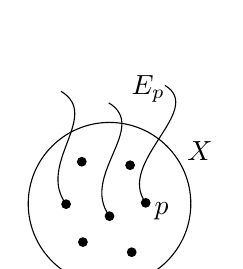
\begin{tikzpicture}[x=0.75pt,y=0.75pt,yscale=-1,xscale=1]

%Shape: Ellipse [id:dp02661356198166054] 
\draw   (175.17,106.61) .. controls (175.17,84.98) and (192.7,67.45) .. (214.33,67.45) .. controls (235.96,67.45) and (253.5,84.98) .. (253.5,106.61) .. controls (253.5,128.24) and (235.96,145.78) .. (214.33,145.78) .. controls (192.7,145.78) and (175.17,128.24) .. (175.17,106.61) -- cycle ;
%Shape: Ellipse [id:dp00618917520895268] 
\draw  [fill={rgb, 255:red, 0; green, 0; blue, 0 }  ,fill opacity=1 ] (198.91,86.38) .. controls (198.91,85.24) and (199.83,84.32) .. (200.97,84.32) .. controls (202.11,84.32) and (203.03,85.24) .. (203.03,86.38) .. controls (203.03,87.52) and (202.11,88.44) .. (200.97,88.44) .. controls (199.83,88.44) and (198.91,87.52) .. (198.91,86.38) -- cycle ;
%Shape: Ellipse [id:dp4985286560152604] 
\draw  [fill={rgb, 255:red, 0; green, 0; blue, 0 }  ,fill opacity=1 ] (191.34,106.82) .. controls (191.34,105.69) and (192.26,104.76) .. (193.4,104.76) .. controls (194.54,104.76) and (195.46,105.69) .. (195.46,106.82) .. controls (195.46,107.96) and (194.54,108.89) .. (193.4,108.89) .. controls (192.26,108.89) and (191.34,107.96) .. (191.34,106.82) -- cycle ;
%Shape: Ellipse [id:dp8690346263253921] 
\draw  [fill={rgb, 255:red, 0; green, 0; blue, 0 }  ,fill opacity=1 ] (222.19,88.07) .. controls (222.19,86.93) and (223.11,86) .. (224.25,86) .. controls (225.39,86) and (226.31,86.93) .. (226.31,88.07) .. controls (226.31,89.2) and (225.39,90.13) .. (224.25,90.13) .. controls (223.11,90.13) and (222.19,89.2) .. (222.19,88.07) -- cycle ;
%Shape: Ellipse [id:dp20263845603499497] 
\draw  [fill={rgb, 255:red, 0; green, 0; blue, 0 }  ,fill opacity=1 ] (212.27,112.61) .. controls (212.27,111.47) and (213.19,110.55) .. (214.33,110.55) .. controls (215.47,110.55) and (216.39,111.47) .. (216.39,112.61) .. controls (216.39,113.75) and (215.47,114.67) .. (214.33,114.67) .. controls (213.19,114.67) and (212.27,113.75) .. (212.27,112.61) -- cycle ;
%Shape: Ellipse [id:dp9834086999067779] 
\draw  [fill={rgb, 255:red, 0; green, 0; blue, 0 }  ,fill opacity=1 ] (229.71,106.19) .. controls (229.71,105.05) and (230.63,104.13) .. (231.77,104.13) .. controls (232.91,104.13) and (233.83,105.05) .. (233.83,106.19) .. controls (233.83,107.33) and (232.91,108.25) .. (231.77,108.25) .. controls (230.63,108.25) and (229.71,107.33) .. (229.71,106.19) -- cycle ;
%Shape: Ellipse [id:dp22592961134490075] 
\draw  [fill={rgb, 255:red, 0; green, 0; blue, 0 }  ,fill opacity=1 ] (199.46,125.11) .. controls (199.46,123.97) and (200.38,123.05) .. (201.52,123.05) .. controls (202.66,123.05) and (203.58,123.97) .. (203.58,125.11) .. controls (203.58,126.25) and (202.66,127.17) .. (201.52,127.17) .. controls (200.38,127.17) and (199.46,126.25) .. (199.46,125.11) -- cycle ;
%Shape: Ellipse [id:dp09074720791053226] 
\draw  [fill={rgb, 255:red, 0; green, 0; blue, 0 }  ,fill opacity=1 ] (222.96,129.98) .. controls (222.96,128.84) and (223.89,127.92) .. (225.03,127.92) .. controls (226.16,127.92) and (227.09,128.84) .. (227.09,129.98) .. controls (227.09,131.12) and (226.16,132.04) .. (225.03,132.04) .. controls (223.89,132.04) and (222.96,131.12) .. (222.96,129.98) -- cycle ;
%Curve Lines [id:da9825824283034781] 
\draw    (190.93,52.44) .. controls (210.59,64.17) and (178.97,87.32) .. (193.4,106.82) ;
%Curve Lines [id:da5263572037731432] 
\draw    (213.96,58.03) .. controls (233.62,69.77) and (199.9,93.11) .. (214.33,112.61) ;
%Curve Lines [id:da6829537734588929] 
\draw    (241.03,49.61) .. controls (260.69,61.34) and (217.34,86.69) .. (231.77,106.19) ;

% Text Node
\draw (223.77,43.4) node [anchor=north west][inner sep=0.75pt]    {$E_{p}$};
% Text Node
\draw (250.62,75.18) node [anchor=north west][inner sep=0.75pt]    {$X$};
% Text Node
\draw (234.77,105.03) node [anchor=north west][inner sep=0.75pt]    {$p$};
\end{tikzpicture}
\eea
\end{itemize}

Roughly speaking, 
\textbf{observables} are functions on fields (or certain homology), in which their space is denoted
$\sO(\cE)$. For example, 
distributions are \emph{linear observables}.
The new structures come from the following facts.
\begin{itemize}
\item Given an open subset $U\subset X$, we can talk about
\bea \on{Obs}(U)= \text{observables supported in } U.\eea

\begin{eg}
$\cE=C^\infty(X),\ p\in X$. Consider 
\bea \cO_1: \cE \to \bR,\eea
where $\cO_1(f)=f(p)^m, \ \forall f\in \cE$. $\cO_1$ is an observable supported in any open neighborhood of $p$.
\end{eg}

\item Let $\cE(U)=\Gamma(U,E)$. Then 
\bea
\on{Obs}(U)=\text{functions on }  \cE(U).
\eea

\item The new structure is the \textbf{factorization product / operator product expansion (OPE)}. Given disjoint open subsets $U_i \subset V$ contained in an open set $V$, such that the disjoint union is $\coprod_i U_i \subset V$, we have a map (factorization product) for observables:
\bea
\bigotimes_i \on{Obs}(U_i)\to \on{Obs}(V).
\eea

\item Intuitively, if $\cE(U)$ is restricted to $\cE(U_i)$, then dually $\sO(\cE(U_i))\to \sO(\cE(U))$.
Naively, we can \emph{multiply} those \emph{functions}, then we get
\bea
\bigotimes_i \on{Obs}(U_i)\to \on{Obs}(V).
\eea
This, however, requires further \emph{quantum corrections} in which fields in $U_i$'s may ``talk'' to each other.

\begin{eg}[Topological Quantum Mechanics (TQM)]
In topological QFT, $\on{Obs}(U)$ only depends on the topology of $U$.
Consider $\on{dim} X=1$ (a 1d QFT is a quantum mechanics) and $\on{Obs}(U)=A$ for any contractible open interval $U$. Now consider two open intervals $U_1$, $U_2$ on $X$ and embed them into a larger interval $V$.
\bea 
\tikzset{every picture/.style={line width=0.75pt}}         
\begin{tikzpicture}[x=0.75pt,y=0.75pt,yscale=-1,xscale=1]


%Straight Lines [id:da49776176722773413] 
\draw    (470,30.46) -- (637.76,30.46) ;
%Straight Lines [id:da7522582205389852] 
\draw    (473.24,105.81) -- (641,105.81) ;
%Straight Lines [id:da9909036802138831] 
\draw    (555.34,46.5) -- (555.34,77.45) ;
\draw [shift={(555.34,79.45)}, rotate = 270] [color={rgb, 255:red, 0; green, 0; blue, 0 }  ][line width=0.75]    (10.93,-3.29) .. controls (6.95,-1.4) and (3.31,-0.3) .. (0,0) .. controls (3.31,0.3) and (6.95,1.4) .. (10.93,3.29)   ;
%Straight Lines [id:da11097180592386091] 
\draw [color={rgb, 255:red, 208; green, 2; blue, 27 }  ,draw opacity=1 ][line width=2.25]    (500,30) -- (549,30) ;
%Straight Lines [id:da6781384757672331] 
\draw [color={rgb, 255:red, 208; green, 2; blue, 27 }  ,draw opacity=1 ][line width=2.25]    (563,30) -- (610,30) ;
%Straight Lines [id:da2471941135880169] 
\draw [color={rgb, 255:red, 144; green, 19; blue, 254 }  ,draw opacity=1 ][line width=2.25]    (500,105.81) -- (610,105.81) ;

% Text Node
\draw (516.34,11) node [anchor=north west][inner sep=0.75pt]   [align=left] {$U_1$};
% Text Node
\draw (577.66,11) node [anchor=north west][inner sep=0.75pt]   [align=left] {$U_2$};
% Text Node
\draw (549.19,87.17) node [anchor=north west][inner sep=0.75pt]   [align=left] {$V$};
\end{tikzpicture}
\eea

We have a topological quantum mechanics (TQM) with maps
\bea
\on{Obs}(U_1)\otimes \on{Obs}(U_2) \to \on{Obs}(V) \quad \text{or} \quad A \otimes A \to A.
\eea
The factorization product does not depend on the location and size. We find an \textbf{associative algebra}!
\end{eg}
\end{itemize}


\paragraph{Algebraic structure.}
Consider two operators being placed at two different points on a line. When one operator approaches closely the other, the algebraic structure of the topology of the line comes from the homology group
\bea
H_{\blt} (\bR-\lcb 0\rcb)=H_0 (\bR-\lcb 0\rcb)= \bZ_{left} \oplus \bZ_{right}
\eea
which comprises the left and right multiplications.
\emph{Associativity} comes from a further consistency:
\bea &
\tikzset{every picture/.style={line width=0.75pt}}         
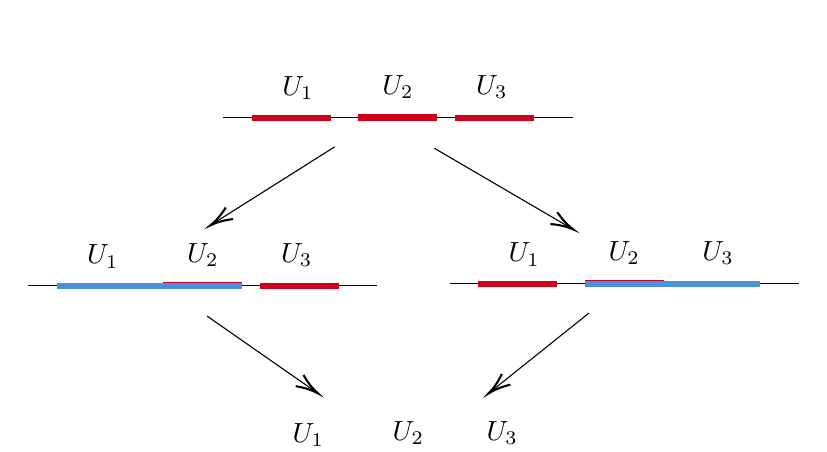
\begin{tikzpicture}[x=0.75pt,y=0.75pt,yscale=-1,xscale=1]
%Straight Lines [id:da5146107324067772] 
\draw    (162.3,64.67) -- (330.54,64.67) ;
%Straight Lines [id:da6366840570335301] 
\draw    (215.94,78.81) -- (157.69,115.6) ;
\draw [shift={(156,116.67)}, rotate = 327.73] [color={rgb, 255:red, 0; green, 0; blue, 0 }  ][line width=0.75]    (10.93,-3.29) .. controls (6.95,-1.4) and (3.31,-0.3) .. (0,0) .. controls (3.31,0.3) and (6.95,1.4) .. (10.93,3.29)   ;
%Straight Lines [id:da4584739157136033] 
\draw    (264,79.51) -- (329.27,117.66) ;
\draw [shift={(331,118.67)}, rotate = 210.3] [color={rgb, 255:red, 0; green, 0; blue, 0 }  ][line width=0.75]    (10.93,-3.29) .. controls (6.95,-1.4) and (3.31,-0.3) .. (0,0) .. controls (3.31,0.3) and (6.95,1.4) .. (10.93,3.29)   ;
%Straight Lines [id:da8016630535031757] 
\draw    (154.51,160.38) -- (206.36,196.52) ;
\draw [shift={(208,197.67)}, rotate = 214.88] [color={rgb, 255:red, 0; green, 0; blue, 0 }  ][line width=0.75]    (10.93,-3.29) .. controls (6.95,-1.4) and (3.31,-0.3) .. (0,0) .. controls (3.31,0.3) and (6.95,1.4) .. (10.93,3.29)   ;
%Straight Lines [id:da5351493584904696] 
\draw    (338.53,158.84) -- (291.56,196.42) ;
\draw [shift={(290,197.67)}, rotate = 321.33] [color={rgb, 255:red, 0; green, 0; blue, 0 }  ][line width=0.75]    (10.93,-3.29) .. controls (6.95,-1.4) and (3.31,-0.3) .. (0,0) .. controls (3.31,0.3) and (6.95,1.4) .. (10.93,3.29)   ;
%Straight Lines [id:da11490255972538899] 
\draw [color={rgb, 255:red, 208; green, 2; blue, 27 }  ,draw opacity=1 ][line width=2.25]    (176,65) -- (214,65) ;
%Straight Lines [id:da38887048079079545] 
\draw [color={rgb, 255:red, 208; green, 2; blue, 27 }  ,draw opacity=1 ][line width=2.25]    (227.42,64.67) -- (265.42,64.67) ;
%Straight Lines [id:da5815548933649641] 
\draw [color={rgb, 255:red, 208; green, 2; blue, 27 }  ,draw opacity=1 ][line width=2.25]    (274,65) -- (312,65) ;
%Straight Lines [id:da045018168844348505] 
\draw    (68.3,145.67) -- (236.54,145.67) ;
%Straight Lines [id:da9494212334866909] 
\draw [color={rgb, 255:red, 208; green, 2; blue, 27 }  ,draw opacity=1 ][line width=2.25]    (82,146) -- (120,146) ;
%Straight Lines [id:da13972709854409504] 
\draw [color={rgb, 255:red, 208; green, 2; blue, 27 }  ,draw opacity=1 ][line width=2.25]    (133.42,145.67) -- (171.42,145.67) ;
%Straight Lines [id:da49239786657156226] 
\draw [color={rgb, 255:red, 208; green, 2; blue, 27 }  ,draw opacity=1 ][line width=2.25]    (180,146) -- (218,146) ;
%Straight Lines [id:da018412058817521393] 
\draw    (271.3,144.67) -- (439.54,144.67) ;
%Straight Lines [id:da8371430474679855] 
\draw [color={rgb, 255:red, 208; green, 2; blue, 27 }  ,draw opacity=1 ][line width=2.25]    (285,145) -- (323,145) ;
%Straight Lines [id:da45745011041205896] 
\draw [color={rgb, 255:red, 208; green, 2; blue, 27 }  ,draw opacity=1 ][line width=2.25]    (336.42,144.67) -- (374.42,144.67) ;
%Straight Lines [id:da59402182478143] 
\draw [color={rgb, 255:red, 208; green, 2; blue, 27 }  ,draw opacity=1 ][line width=2.25]    (383,145) -- (421,145) ;
%Straight Lines [id:da3383677142840795] 
\draw    (167.3,231.67) -- (335.54,231.67) ;
%Straight Lines [id:da30399344382391535] 
\draw [color={rgb, 255:red, 208; green, 2; blue, 27 }  ,draw opacity=1 ][line width=2.25]    (181,232) -- (219,232) ;
%Straight Lines [id:da8362418177389068] 
\draw [color={rgb, 255:red, 208; green, 2; blue, 27 }  ,draw opacity=1 ][line width=2.25]    (232.42,231.67) -- (270.42,231.67) ;
%Straight Lines [id:da10310047941667388] 
\draw [color={rgb, 255:red, 208; green, 2; blue, 27 }  ,draw opacity=1 ][line width=2.25]    (279,232) -- (317,232) ;
%Straight Lines [id:da8603812711814927] 
\draw [color={rgb, 255:red, 74; green, 144; blue, 226 }  ,draw opacity=1 ][line width=2.25]    (82,146) -- (171.42,146) ;
%Straight Lines [id:da6924243205034588] 
\draw [color={rgb, 255:red, 74; green, 144; blue, 226 }  ,draw opacity=1 ][line width=2.25]    (336.42,145) -- (421,145) ;
%Straight Lines [id:da35290975414233494] 
\draw [color={rgb, 255:red, 144; green, 19; blue, 254 }  ,draw opacity=1 ][line width=2.25]    (181,232) -- (317,232) ;

% Text Node
\draw (189.46,43.85) node [anchor=north west][inner sep=0.75pt]   [align=left] {$U_1$};
% Text Node
\draw (237.64,43) node [anchor=north west][inner sep=0.75pt]   [align=left] {$U_2$};
% Text Node
\draw (282.83,43) node [anchor=north west][inner sep=0.75pt]   [align=left] {$U_3$};
% Text Node
\draw (95.46,124.85) node [anchor=north west][inner sep=0.75pt]   [align=left] {$U_1$};
% Text Node
\draw (143.64,124) node [anchor=north west][inner sep=0.75pt]   [align=left] {$U_2$};
% Text Node
\draw (188.83,124) node [anchor=north west][inner sep=0.75pt]   [align=left] {$U_3$};
% Text Node
\draw (298.46,123.85) node [anchor=north west][inner sep=0.75pt]   [align=left] {$U_1$};
% Text Node
\draw (346.64,123) node [anchor=north west][inner sep=0.75pt]   [align=left] {$U_2$};
% Text Node
\draw (391.83,123) node [anchor=north west][inner sep=0.75pt]   [align=left] {$U_3$};
% Text Node
\draw (194.46,210.85) node [anchor=north west][inner sep=0.75pt]   [align=left] {$U_1$};
% Text Node
\draw (242.64,210) node [anchor=north west][inner sep=0.75pt]   [align=left] {$U_2$};
% Text Node
\draw (287.83,210) node [anchor=north west][inner sep=0.75pt]   [align=left] {$U_3$};
\end{tikzpicture} \\ 
&\Longrightarrow (a\cdot b)\cdot c= a\cdot (b\cdot c),\quad a,b,c\in \text{Obs}(U_i),\ i=1,2,3.
\eea

\begin{eg}[Chiral QFT] Let $\on{dim }X=2$. The factorization product of a two-dimensional (2d) chiral theory is \textbf{holomorphic}.
\bea 
\tikzset{every picture/.style={line width=0.75pt}}     
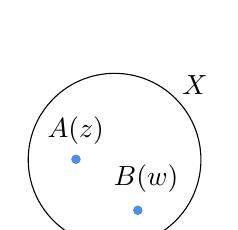
\begin{tikzpicture}[x=0.75pt,y=0.75pt,yscale=-1,xscale=1]

%Shape: Circle [id:dp46405244436709836] 
\draw  [color={rgb, 255:red, 74; green, 144; blue, 226 }  ,draw opacity=1 ][fill={rgb, 255:red, 74; green, 144; blue, 226 }  ,fill opacity=1 ] (144.8,123.47) .. controls (144.8,122.36) and (145.7,121.47) .. (146.8,121.47) .. controls (147.9,121.47) and (148.8,122.36) .. (148.8,123.47) .. controls (148.8,124.57) and (147.9,125.47) .. (146.8,125.47) .. controls (145.7,125.47) and (144.8,124.57) .. (144.8,123.47) -- cycle ;
%Shape: Ellipse [id:dp6198652930020687] 
\draw   (94,99.07) .. controls (94,76.09) and (112.62,57.47) .. (135.6,57.47) .. controls (158.58,57.47) and (177.2,76.09) .. (177.2,99.07) .. controls (177.2,122.04) and (158.58,140.67) .. (135.6,140.67) .. controls (112.62,140.67) and (94,122.04) .. (94,99.07) -- cycle ;
%Shape: Ellipse [id:dp42367483552549756] 
\draw  [color={rgb, 255:red, 74; green, 144; blue, 226 }  ,draw opacity=1 ][fill={rgb, 255:red, 74; green, 144; blue, 226 }  ,fill opacity=1 ] (115,98.87) .. controls (115,97.76) and (115.9,96.87) .. (117,96.87) .. controls (118.1,96.87) and (119,97.76) .. (119,98.87) .. controls (119,99.97) and (118.1,100.87) .. (117,100.87) .. controls (115.9,100.87) and (115,99.97) .. (115,98.87) -- cycle ;

% Text Node
\draw (102.06,77.07) node [anchor=north west][inner sep=0.75pt]    {$A( z)$};
% Text Node
\draw (134,100.27) node [anchor=north west][inner sep=0.75pt]    {$B( w)$};
% Text Node
\draw (167,57.07) node [anchor=north west][inner sep=0.75pt]    {$X$};
\end{tikzpicture}
\eea

\noindent In holomorphic coordinates, when an operator approach (or wind around) the other on $X$, the winding number can be kept track in terms of their Fourier/Laurent modes:
\bea 
A(z)B(w)=\sum_{n\in \bZ}\frac{\lb A_{(n)} B\rb (w)}{(z-w)^{n+1}}.
\eea
We find $\infty$-ly many ``products'' (or binary operations) $\lcb A_{(n)} B \rcb$. In this case, the observable algebra gives rise to a \textbf{vertex algebra}.
\end{eg}

Observable algebras are developed in the works of:
\begin{itemize}
    \item Beilinson-Drinfeld \cite{beilinson2004chiral}
    \begin{itemize}
        \item developed \textbf{factorization algebra} to formulate 2d chiral conformal field theory (CFT),
        \item introduced the notion of \textbf{chiral homology} (generalizing \emph{Hochschild homology} in one dimension).
    \end{itemize}
    \item Costello-Gwilliam \cite{costello2021factorization}
    \begin{itemize}
        \item constructed factorization algebras from perturbative renormalization theory, in the \textbf{Batalin-Vilkovisky (BV) formalism} \cite{BATALIN198127} (generalizing \emph{BRST formalism} in gauge theory).
    \end{itemize}
\end{itemize}

%\begin{rmk} The geometrical study of QFT are related to index theory: 1-dim. (Atiyah-Singer index theory), 2-dim. (chiral index theory on loop space). (see later) \end{rmk}

\subsection{BV formalism and homological integration}
Now we want to construct a homotopic renormalization in the perturbative BV formalism. The basic idea is formulated via the homological interpretation of integral, 
    \bea \boxed{\int \ =\ \text{homology}}\ .\eea
\paragraph{Calculus revisited.}
    Calculus is nicely packaged into the framework of de Rham theory. Let $M$ be a compact oriented manifold of $\on{dim} M=n$. Many constructions of integration on manifolds can be understood from de Rham complex
    $\lb \Omega^\blt(M), d\rb$, where $\Omega^\blt(M)$ is the space of smooth differential forms and $d$ is the de Rham differential. There is a natural integration map 
    \bea
    \int_M: \Omega^\blt(M) \to \bR,\quad
    \alpha\in \Omega^n(M) \mapsto \int_M \alpha\in \bR. \eea
    Observe that the $n$-th de Rham cohomology group
    $H^n_{dR}(M) =H^n\lb \Omega^\blt(M),d\rb\simeq\bR$. This implies that 
    \bea
    \int_M \ = \ H^n_{dR}. \eea
    The integration map is now
    \bea
    \Omega^n(M) \to H^n_{dR}(M),\quad
    \alpha \mapsto [\alpha].
    \eea
    This means that we can learn calculus by the algebraic structure on de Rham complex, even we do not know anything about measure theory. However, there is a problem of understanding $H^n_{dR}(M)$ when $n\to\infty$ as in QFT.
    
\paragraph{BV approach.}
    Define \textbf{polyvector fields}
    \bea 
    \on{PV}^\blt(M) =\bigoplus_k \on{PV}^k(M)\coloneqq \bigoplus_k \Gamma \lb M,\ \asym^k TM\rb.
     \eea
    Let $\Omega$ be a fixed volume form on $M$. We can naturally identify
    \bea
    \on{PV}^k(M) \xleftrightarrow{\ \lrcorner \Omega\ } \Omega ^{n-k}(M),\quad
    \mu\in \on{PV}^k(M) \lra \mu \lrcorner \Omega.
    \eea
    Locally, if $\Omega=e^\varphi dx^1\wedge \cdots \wedge dx^n$, $\mu=\mu^{i_1\cdots i_k} \partial_{i_1}\wedge \cdots \wedge \partial_{i_k}$, then
    \bea \mu \lrcorner\Omega= \sum \pm \mu^{i_1\cdots i_k} e^\varphi dx^1 \wedge \cdots \wedge \widehat{dx^{i_1}}\wedge \cdots \wedge\widehat{dx^{i_k}} \wedge \cdots \wedge dx^n. \eea
    
    %%%%%%%%%%%%%%%%%%%%%%%%%%%%%%%%%%%%
    The identification above leads to 
    \bea
    \begin{tikzcd}
    \Omega^{0} \ar[r, "d"] \ar[dd, "\simeq"] 
    & \Omega^{1} \ar[r, "d"] \ar[dd, "\simeq"] 
    & \cdots \ar[r,"d"] & \Omega^{n} \ar[dr, "\int"] \ar[dd, "\simeq"] & \\
     & & & & \bR \\
    PV^{n} \ar[r, "\Delta"]
    & PV^{n-1} \ar[r, "\Delta"]
    & \cdots \ar[r, "\Delta"] & PV^{0}  \ar[ur, swap, "\int_{BV}"] & 
    \end{tikzcd}
    \eea
where
$\Delta: \on{PV}^k \to \on{PV}^{k-1}$ is a divergence operator with respect to $\Omega$. $\Delta$ is called the \textbf{BV operator}, induced from the de Rham differential operator $d$.
For example, 
$\Delta: \on{PV}^1=\on{Vect}(M) \to \on{PV}^0=C^\infty(M)$ is the usual divergence.

$\int_{BV}$ is the \textbf{BV integration}, which is a map
\bea \int_{BV}: \on{PV}^0 \to \bR,\quad 
f \mapsto \int f\Omega.
\eea
Homologically $\int_{BV}$ can be identified with $H^0_{BV}$, i.e. \bea \boxed{\int_{BV}= H^0}\ .\eea
Here ``$\on{dim} (M)$'' does not appear. The problem of integration is transferred to construct $\Delta$, which has a convenient formulation at least in perturbative QFT. This is one of the folklore advantage of working with BV.
The challenge now is to construct $\Delta$ in the $\infty$-dimensional setting.
In $\infty$ dimensions (as in QFT), renormalization helps to construct $\Delta$, leading to a \textbf{homological integration}.

\paragraph{Explicit form of $\Delta$.}
Locally in $U$, let $\lcb x_i\rcb_{i=1}^n$ be local coordinates and $\Omega=e^{f(x)}dx^1\wedge \cdots \wedge dx^n$ be the volume form. Introduce the vector fields $\partial_i=\frac{\partial}{\partial x_i}$, then the polyvector field is \bea \on{PV}(U)=C^\infty(U) [\partial_1, \cdots, \partial_n],\eea
where $\partial_i$'s are anticommuting: $\partial_i \partial_j =- \partial_j \partial_i$. 
Let us write $\theta_i=\partial_i$ (\textit{note}: this is a vector field, NOT an differential operator), then a local section $\mu\in \on{PV}(X)$ can be written as a function of $x^i$, $\theta_i$:
\bea
\mu=\mu (x^i, \theta_i)
\eea
with $x^ix^j=x^j x^i$ and $\theta_i \theta_j =- \theta_j \theta_i$.
Let $\frac{\partial}{\partial x^i}$ be the derivative with respect to $x^i$  and $\frac{\partial}{\partial \theta_i}$ be the derivative with respect to $\theta_i$ (from the left). Then the BV operator is given locally by 
\bea
\Delta = \sum_i \frac{\partial}{\partial x^i} \frac{\partial}{\partial \theta_i}
+\sum_i (\partial_i f) \frac{\partial}{\partial \theta_i}
\eea
which looks like a second order operator (it is easy to check that $\Delta^2=0$). This is in contrast with de Rham differential $d$, which is a first order differential
operator. Note that the first term looks like a Laplacian, but it is NOT. $\theta_i$ is an odd variable. Hence, $\Delta$ is sometimes called an \emph{odd Laplacian}.

\begin{eg}[$\frac{\partial}{\partial \theta_i}$ operator]
\bea\frac{\partial}{\partial \theta_1}(\theta_1\theta_2) &=\theta_2,\\
\frac{\partial}{\partial \theta_1}(\theta_2\theta_1) &=- \frac{\partial}{\partial \theta_1}(\theta_1\theta_2)=-\theta_2.
\eea
\end{eg}

\begin{eg}[Singularity theory: an example of $\int_{BV}$]
Consider the $n$-dimensional complex space $\bC^n$. Let $f(z^i): \bC^n\to \bC$ be a polynomial in $n$ variables with an isolated critical point at the origin, 0:
\bea \on{Crit}(f)=\lcb 0\rcb.\eea
We consider holomorphic/polynomial polyvector fields
\bea \cA =\bC[z^i, \theta_i], \quad
\theta_i \theta_j =- \theta_j \theta_i.\eea
Let the BV operator be
\bea \Delta=\hbar \sum_{i=1}^n \frac{\partial}{\partial z^i} \frac{\partial}{\partial \theta_i}
+\sum_i (\partial_i f) \frac{\partial}{\partial \theta_i}. \eea
\begin{itemize}
    \item $f(z^i)$ gives a solution of the quantum master equation (QME) in $\cA[[\hbar]]$: $\Delta f = \lcb f, f\rcb = 0$.
    \item The space of quantum observables, $\on{Obs}^q=H^\blt (\cA [[  \hbar]], \hbar\Delta+\lcb f,-\rcb)$, is isomorphic to a formal completion of the Brieskorn lattice \cite{saito1983higher}.
    \item 
    The quantum observable (or Brieskorn lattice) plays an important role of Hodge filtration (which is related to $\hbar$-filtration) in singularity theory (see \cite{arnold2012singularities,kulikov1998mixed} for an exposition).
    \item The BV-integration models the oscillatory integral 
    \bea \lan \cO\ran=\int_{\mathcal{L}} d^n z\ \cO e^{f/\hbar},\eea where $\mathcal{L}$ is a Lefschetz thimble.
    \item The above finite-dimensional model is the effective theory of topological Landau-Ginzburg B-model. 
    \item In general, a QFT can be viewed as a version of $\infty$-dimensional singularity theory.
\end{itemize}
\end{eg}

\noindent \textsc{Reference}: \cite{Li:2017exk}.

\section{Perturbative theory and Feynman diagram}\label{sec:ptfd}
Understanding the path integral $\int e^{-S/\hbar}$ on the full space of fields is difficult. We can, however, have a well understanding of the behavior of a theory around the critical points of the action functional $S$. We will work on the asymptotic $\hbar$-expansion around the minima of $S$. This perturbative theory has a very nice combinatorial expression --- Feynman diagrams, which also has physical interpretations. We present this result via the {\em BV idea}. This idea is different from the usual approach to Feynman diagrams, but it has an advantage that its homological interpretation can be used in formulating index theory.

As discussed in the \nameref{sec:intro}, given a volume form
\bea \Omega=e^{f(x)} dx^1\wedge \cdots \wedge dx^n,\eea
we can consider the integration map 
\bea
\int: \ \cA
\to \bR,\eea
where $\cA$ is a function on $\lcb x^i,\theta_i\rcb$, where $\theta_i$'s are anticommuting variables, $\theta_i \theta_j =- \theta_j \theta_i$. 
If we integrate over $\bR^n$, $\int_{\bR^n}$ picks only the components without $\theta_i$'s (i.e. the $\on{PV}^0$-part) and
\bea \int_{\bR^n}: f(x)\mapsto \int_{\bR^n} f(x)\Omega.\eea
This integration is defined on BV homology ($\Delta$-homology), where 
$\Delta: \cA \to \cA$ is the BV-operator given by
\bea \Delta= \sum_{i=1}^n \frac{\partial}{\partial x^i} \frac{\partial}{\partial \theta_i}
+\sum_i (\partial_i f) \frac{\partial}{\partial \theta_i}. \eea

\begin{eg} An integral over a $\Delta$-exact term vanishes, i.e.
\bea\int_{\bR^n}\Delta(\varphi^i(x)\theta_i)\Omega=0.\eea
This looks like the Stokes' theorem.
Explicitly,
\bea\int_{\bR^n} d^n x \lb \sum_i \partial_i\varphi^i+\sum_i \varphi^i\partial_i f\rb e^f =0. \eea
It vanishes after the integration by part is performed.
\end{eg}

\subsection*{Gaussian integral}
Consider the simplest example: a one-dimensional real space $\bR$ and a Gaussian-type volume form
\bea \Omega= \frac{1}{\sqrt{2\pi}} e^{-\hf x^2} dx.\eea
We study the integration map on polynomial functions:
\bea\int: \ \bR[x]\to \bC,\qquad g(x)\mapsto\int_\bR g(x)\Omega \eea
or more generally,
\bea\int: \ \bR[x,\theta]\to \bC,\qquad g(x)+h(x)\theta \mapsto\int_\bR g(x)\Omega \qquad (\theta^2=0).\eea
The BV operator reads
\bea
\Delta = \frac{\partial}{\partial x} \frac{\partial}{\partial \theta}
-x \frac{\partial}{\partial \theta}.
\eea
Here $f= -\hf x^2$. Given any polynomial $g(x)\in \bR[x]$, we have
\bea \Delta g=0\eea
since $g$ has no $\theta$'s. Let $[g]_{\Delta}$ denote the \textbf{$\Delta$-cohomology classes}, in which
\bea
\lsb g_1\rsb_{\Delta}=\lsb g_2\rsb_{\Delta}\ \LRA \ g_1-g_2=\Delta \eta \ \text{for some } \eta\in \bR[x,\theta].
\eea
Then $\int$ is well-defined on $\Delta$-cohomology classes:
\bea \int g_1\Omega= \int g_2\Omega \quad  \text{if } 
\lsb g_1\rsb_{\Delta}=\lsb g_2\rsb_{\Delta}.\eea
We also have the normalization of the Gaussian integral:
\bea \int 1\ \Omega =1.\eea

\begin{eg}
\bea \Delta \lb x^{m-1}\theta\rb &=
\lb\frac{\partial}{\partial x} \frac{\partial}{\partial \theta}
-x \frac{\partial}{\partial \theta}\rb \lb x^{m-1}\theta\rb
=(m-1)x^{m-2} -x^m\\
\RA \lsb x^m\rsb_{\Delta} &= (m-1) \lsb x^{m-2}\rsb_{\Delta}\\
\RA \lsb x^{2k}\rsb_{\Delta} &= (2k-1)!! \lsb 1\rsb_{\Delta}\\
\RA \int_{\bR} x^{2k}\Omega &= 
(2k-1)!! \int_{\bR}\Omega= 
(2k-1)!!.\eea
\end{eg}

\subsection*{Conjugation}
To organize the data, consider the following operator
\bea \cU=e^{\hf \frac{\partial}{\partial x} \frac{\partial}{\partial x}}: \bR\lsb x,\theta\rsb \to \bR\lsb x,\theta\rsb.\eea
Explicitly, $\cU\lb g(x)+h(x)\theta\rb= 
\lb \cU g(x)\rb+ \lb \cU h(x)\rb \theta,$ where $\cU$ acts on polynomials via Taylor expansion
\bea \cU=\sum_{k=0}^\infty \frac{1}{k!} \lb \hf \frac{\partial}{\partial x} \frac{\partial}{\partial x} \rb^k \eea
which is well-defined on $\bR[x]$.

\begin{lem}
The BV operator is given by
\bea \Delta= \cU^{-1}\lb -x\frac{\partial}{\partial\theta}\rb \cU\eea
i.e. $\Delta$ is conjugate to the simple operation $-x\frac{\partial}{\partial\theta}$ via the operator $\cU$.
\end{lem}
\begin{proof}
Exercise.
\end{proof}


As a result, we find a {\em cochain isomorphism} of complexes
\bea \cU: \lb \bR\lsb x,\theta\rsb,\Delta\rb \to \lb \bR\lsb x,\theta\rsb,-x\frac{\partial}{\partial\theta}\rb, \qquad 1\mapsto 1.
\eea
Cochain map means that
\bea \cU \circ \Delta(\varphi)= \lb -x\frac{\partial}{\partial\theta}\rb\circ \cU(\varphi) \eea
i.e. $\cU$ intertwines $\Delta$ with $-x\frac{\partial}{\partial\theta}$.

Observe that
\bea
H^\blt \lb \bR\lsb x,\theta \rsb, 
-x\frac{\partial}{\partial\theta}\rb
=H^0 \lb \bR\lsb x,\theta \rsb, 
-x\frac{\partial}{\partial\theta}\rb=\bR.
\eea
Let $\lsb -\rsb_{-x\partial_\theta}$ represent the $\lb -x\frac{\partial}{\partial\theta}\rb$-cohomology classes. Then for any $m>0, x^m=\lb -x\frac{\partial}{\partial\theta}\rb \lb-x^{m-1}\theta\rb$. Hence,
\bea \lsb h(x)\rsb_{-x\partial_\theta}= \lsb h(0)\rsb_{-x\partial_\theta}\eea
for an arbitrary polynomial $h(x)$. All higher power terms beyond the constant terms are exact; hence they vanish.
Now for any $g(x)\in \bR\lsb x\rsb$,
\bea
\begin{tikzcd}
\lsb g(x)\rsb_{\Delta} \ar[r, "\cU"] \ar[equal]{d}
& \lsb \cU( g(x))\rsb_{-x\partial_{\theta}} \ar[equal]{d} \\
\cU(g)(0)\lsb 1\rsb_{\Delta} 
& \lsb \cU(g(0))\rsb_{-x\partial_{\theta}} \ar[l]
\end{tikzcd}
\eea
we find 
\bea \lsb g(x)\rsb_{\Delta}= \cU(g)(0)\lsb 1\rsb_{\Delta}.\eea
In other words, 
\bea
\int_{\bR} g(x)\Omega\ =\left. e^{\hf \partial_x^2} g(x)\right|_{x=0} \int_{\bR} 1\Omega \ =\left. e^{\hf \partial_x^2} g(x)\right|_{x=0}.
\eea

In general, we can introduce a new parameter $a$. 
\begin{prop}\label{prop1}
\bea \int_\bR g(x+a)\Omega = e^{\hf \partial_a^2}g(a),\quad  \forall g\in \bR[x].\eea
\end{prop}
\noindent The shift by $a$ has the interpretation of effective fields as well as background fields, which is related to homological perturbation. The upshot now is that the integration $\int \lb\cdots \rb \Omega$ is fully described by the operator $\cU$.

Now we consider a toy model:
\bea
\int_\bR \frac{dx}{\sqrt{2\pi\hbar}}\ e^{\lb -\hf x^2+\frac{\lambda}{3!}x^3\rb /\hbar}, \quad x, \lambda\in\bR.
\eea
This integral is in fact divergent since $x^3$ blows up quickly at $\infty$. There are two ways out of this problem. 
\bi[(1)]
    \item Treat $x$ as a complex variable and change the integration cycle from $\bR$ (i.e. $\Re(x)$) to some integration cycles $\Gamma_i\in \bC$:
    \bea \int_{\Gamma_i}\frac{dx}{\sqrt{2\pi\hbar}}\ e^{\lb -\hf x^2+\frac{\lambda}{3!}x^3\rb /\hbar}, \quad x\in\bC,\ \lambda\in\bR.\eea
    
\bea
\tikzset{every picture/.style={line width=0.75pt}} %set default line width to 0.75pt    
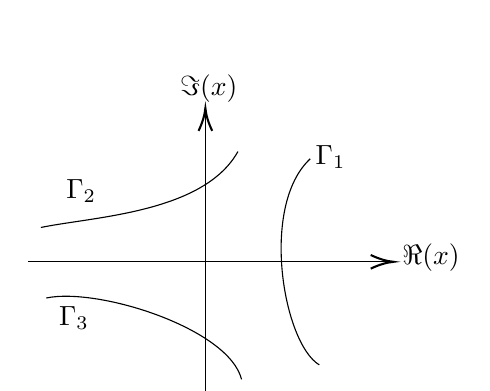
\begin{tikzpicture}[x=0.75pt,y=0.75pt,yscale=-1,xscale=1]
%uncomment if require: \path (0,300); %set diagram left start at 0, and has height of 300

%Straight Lines [id:da772733815126962] 
\draw    (127.35,195) -- (127.35,53.29) ;
\draw [shift={(127.35,51.29)}, rotate = 90] [color={rgb, 255:red, 0; green, 0; blue, 0 }  ][line width=0.75]    (10.93,-3.29) .. controls (6.95,-1.4) and (3.31,-0.3) .. (0,0) .. controls (3.31,0.3) and (6.95,1.4) .. (10.93,3.29)   ;
%Straight Lines [id:da03837733772961949] 
\draw    (42,125.32) -- (215.94,125.32) ;
\draw [shift={(217.94,125.32)}, rotate = 180] [color={rgb, 255:red, 0; green, 0; blue, 0 }  ][line width=0.75]    (10.93,-3.29) .. controls (6.95,-1.4) and (3.31,-0.3) .. (0,0) .. controls (3.31,0.3) and (6.95,1.4) .. (10.93,3.29)   ;
%Curve Lines [id:da1873702300348834] 
\draw    (177.87,75.68) .. controls (153.48,98.32) and (164.81,164.52) .. (182.23,174.97) ;
%Curve Lines [id:da9465928462718054] 
\draw    (143.03,72.19) .. controls (126.48,101.81) and (73.35,103.55) .. (48.1,108.77) ;
%Curve Lines [id:da48991182789985976] 
\draw    (144.77,181.94) .. controls (138.68,157.55) and (75.97,137.52) .. (50.71,142.74) ;

% Text Node
\draw (179.26,67.95) node [anchor=north west][inner sep=0.75pt]    {$\Gamma _{1}$};
% Text Node
\draw (59.06,84.5) node [anchor=north west][inner sep=0.75pt]    {$\Gamma _{2}$};
% Text Node
\draw (55.58,145.46) node [anchor=north west][inner sep=0.75pt]    {$\Gamma _{3}$};
% Text Node
\draw (220.97,115.11) node [anchor=north west][inner sep=0.75pt]    {$\Re ( x)$};
% Text Node
\draw (113.9,34.11) node [anchor=north west][inner sep=0.75pt]    {$\Im ( x)$};
\end{tikzpicture}
\eea
    This becomes the Airy integral. 
    
    \item Treat the integral as an asymptotic series in $\lambda$ via
    \bea e^{\frac{\lambda}{3!\hbar}x^3}= \sum_{n\geq 0} \frac{\lb \frac{\lambda}{3!\hbar}x^3\rb^n}{n!}.\eea
\ei

\subsection*{Perturbative theory}
Let's focus on method (2). This is known as the {\em perturbative theory}. We will also add the background parameter $a$ in our integral.
\bea \int_\bR \frac{dx}{\sqrt{2\pi\hbar}}\ e^{\lb -\hf x^2+\frac{\lambda}{3!}(x+a)^3\rb /\hbar}
\ =\ e^{\frac{\hbar}{2}\partial_a^2} e^{\frac{\lambda}{3!\hbar}a^3}
\ =\ \sum_{k,m\geq 0} 
\frac{\lb \frac{\hbar}{2}\partial_a^2\rb^k}{k!}
\frac{\lb  \frac{\lambda}{3!\hbar}a^3\rb^m}{m!}.
\eea
We have used the fact (Proposition \ref{prop1}) that the integration $\int_\bR \frac{dx}{\sqrt{2\pi\hbar}} g(x+a) e^{-\frac{1}{2\hbar} x^2}$ is described by the operator $e^{\frac{\hbar}{2} \partial_a^2}g(a)$. This infinite sum can be organized into graphs (or Feynman diagrams). Here are some examples.
\begin{itemize}
    \item one term in $\lb \frac{\hbar}{2}\partial_a^2\rb^2
    \lb \frac{\lambda}{3!\hbar}a^3\rb^2$ has
    \bea
    \begin{fmffile}{fd1}
    \begin{tabular}{c}
        \begin{fmfgraph*}(120,70)
                \fmfleft{i}
                \fmfright{o}
                \fmf{plain,tension=4}{i,v1}
                \fmf{plain,tension=4}{v2,o}
                \fmf{plain,left,label=$\frac{\hbar}{2}\partial_a\otimes\partial_a$,label.side=left,tension=1}{v1,v2,v1}
                \fmfv{label=$\frac{\lambda}{\hbar}$,label.angle=120,decor.shape=circle,decor.filled=full,decor.size=2thick}{v1}
                \fmfv{label=$\frac{\lambda}{\hbar}$,label.angle=60,decor.shape=circle,decor.filled=full,decor.size=2thick}{v2}
                \fmflabel{$a$}{i}
                \fmflabel{$a$}{o}
        \end{fmfgraph*}
        \end{tabular}
    \end{fmffile}
    ~~~~~~~~ \sim\ \lambda^2 a^2,
    \eea
    
    \item one term in $\lb \frac{\hbar}{2}\partial_a^2\rb
    \lb \frac{\lambda}{3!\hbar}a^3\rb^2$ has
    \bea
    \begin{fmffile}{fd2}
    \begin{tabular}{c}
        \begin{fmfgraph*}(120,70)
                \fmfleft{i1,i2}
                \fmfright{o1,o2}
                \fmf{plain,tension=.5}{i1,v1}
                \fmf{plain,tension=.5}{i2,v1}
                \fmf{plain,tension=.5}{v2,o1}
                \fmf{plain,tension=.5}{v2,o2}
                \fmf{plain,label=$\hbar \partial_a\otimes\partial_a$,label.side=left,tension=.4}{v1,v2}
                \fmfv{label=$\frac{\lambda}{\hbar}$,label.angle=180,decor.shape=circle,decor.filled=full,decor.size=2thick}{v1}
                \fmfv{label=$\frac{\lambda}{\hbar}$,label.angle=0,decor.shape=circle,decor.filled=full,decor.size=2thick}{v2}
                \fmflabel{$a$}{i1}
                \fmflabel{$a$}{i2}
                \fmflabel{$a$}{o1}
                \fmflabel{$a$}{o2}
        \end{fmfgraph*}
        \end{tabular}
    \end{fmffile}
    ~~~~~~~~ \sim\ \frac{\lambda^2}{\hbar}a^4.
    \eea
\end{itemize}

In general, given a graph $\Gamma$, let
\bea
D &=\text{number of external edges},\\
E &=\text{number of internal edges},\\
V &=\text{number of vertices}.\\
\eea
Define a \textbf{weight function} 
\bea W_{\Gamma}(a) \coloneqq a^D\lambda^V \hbar^{E-V}.\eea
For a connected graph $\Gamma$, we have
\bea V-E= \chi(\Gamma)=1-\ell,\eea
where $\chi$ is the Euler characteristic of the graph $\Gamma$ and $\ell$ is the number of loops. Then
\bea
W_{\Gamma}(a)=a^D \lambda^V \hbar^{\ell-1}.\eea

\begin{eg}
\bea
    \begin{fmffile}{fd3}
    \begin{tabular}{c}
        \begin{fmfgraph*}(80,40)
                \fmfleft{i}
                \fmfright{o}
                \fmf{plain,tension=4}{i,v1}
                \fmf{plain,tension=4}{v2,o}
                \fmf{plain,left,tension=2}{v1,v2,v1}
                \fmfv{decor.shape=circle,decor.filled=full,decor.size=2thick}{v1}
                \fmfv{decor.shape=circle,decor.filled=full,decor.size=2thick}{v2}
        \end{fmfgraph*}
        \end{tabular}
    \end{fmffile}
    ~~~~~~~~ D=2, E=2, V=2 \RA \ell=1.
    \\ \\ 
    \begin{fmffile}{fd4}
    \begin{tabular}{c}
        \begin{fmfgraph*}(80,40)
                \fmfleft{i1,i2}
                \fmfright{o1,o2}
                \fmf{plain,tension=.5}{i1,v1}
                \fmf{plain,tension=.5}{i2,v1}
                \fmf{plain,tension=.5}{v2,o1}
                \fmf{plain,tension=.5}{v2,o2}
                \fmf{plain,tension=.4}{v1,v2}
                \fmfv{decor.shape=circle,decor.filled=full,decor.size=2thick}{v1}
                \fmfv{decor.shape=circle,decor.filled=full,decor.size=2thick}{v2}
        \end{fmfgraph*}
        \end{tabular}
    \end{fmffile}
    ~~~~~~~~ D=4, E=1, V=2 \RA \ell=0.
    \eea
\end{eg}

\begin{prop}[Feynman diagram expansion formula]
\bea \int_\bR \frac{dx}{\sqrt{2\pi\hbar}}\ e^{\lb -\hf x^2+\frac{\lambda}{3!}(x+a)^3\rb /\hbar}
\ =\ e^{\frac{\hbar}{2}\partial_a^2} e^{\frac{\lambda}{3!\hbar}a^3}
\ =\ \on{exp}\lb \sum_{\Gamma:\text{ connected trivalent graph}} \frac{W_\Gamma(a)}{\left| \on{Aut}(\Gamma)\right|}\rb.\eea
Here $\on{Aut}(\Gamma)$ is the automorphism group of $\Gamma$. 
\end{prop}

If we define
\bea W(a) &=\hbar \sum_{\Gamma:\text{ connected graph}} \frac{W_\Gamma(a)}{\left| \on{Aut}(\Gamma)\right|}\\
&=\sum_{g\geq 0}W_g(a)\hbar^g \qquad (\text{expansion in } \hbar).\eea
Here $\hbar W_\Gamma(a)\sim \hbar^{E-V+1}=\hbar^\ell.$ Then we can write the above formula as
\bea
e^{W(a)/\hbar}=\int_{\bR} \frac{dx}{\sqrt{2\pi\hbar}}\ e^{-\frac{1}{2\hbar}x^2} e^{I(x+a)/\hbar}
\eea
for $I(x)=\frac{\lambda x^3}{3!}$ is the cubic \textbf{interaction}. We can further write it as 
\bea e^{W(a)/\hbar}=e^{\frac{\hbar}{2}\partial_a^2} e^{I(a)/\hbar}\eea
and $e^{\frac{\hbar}{2}\partial_a^2}$ plays the role of \textbf{integration}. In physics terminology, we have the operator called the \textbf{propagator}:
\bea P\coloneqq \hf \partial_x^2.\eea
Define a transformation on $I(x)$:
\bea I\mapsto W(P,I)\eea
by the equation
\bea e^{W(P,I)/\hbar}\coloneqq e^{\hbar P}e^{I/\hbar}.\eea
Similarly, we have a graph formula
\bea
W(P,I)=\hbar \sum_{\Gamma:\text{ connected graph}} \frac{W_\Gamma}{\left| \on{Aut}(\Gamma)\right|}.\\
\eea
In general, $I(x)$ involves higher power interaction terms. For example, we have 
\bea
    \begin{fmffile}{fd5}
    \begin{tabular}{c}
        \begin{fmfgraph*}(80,40)
                \fmfleft{i}
                \fmfright{o}
                \fmf{plain,tension=4}{i,v1}
                \fmf{plain,tension=4}{v2,o}
                \fmf{plain,left,label.side=left,tension=2}{v1,v2,v1}
                \fmfv{decor.shape=circle,decor.filled=full,decor.size=2thick}{v1}
                \fmfv{decor.shape=circle,decor.filled=full,decor.size=2thick}{v2}
        \end{fmfgraph*}
        \end{tabular}
    \end{fmffile}
    ~~ + ~~
    \begin{fmffile}{fd6}
    \begin{tabular}{c}
        \begin{fmfgraph*}(80,40)
                \fmfleft{i1,i2}
                \fmfright{o1,o2}
                \fmf{plain,tension=4}{i1,v1}
                \fmf{plain,tension=4}{i2,v1}
                \fmf{plain,tension=4}{v2,o1}
               \fmf{plain,tension=4}{v2,o2} \fmf{plain,left,label.side=left,tension=3}{v1,v2,v1}
                \fmfv{decor.shape=circle,decor.filled=full,decor.size=2thick}{v1}
                \fmfv{decor.shape=circle,decor.filled=full,decor.size=2thick}{v2}
        \end{fmfgraph*}
        \end{tabular}
    \end{fmffile}
    ~~ +\ \cdots. ~~
\eea

\begin{prop}
$W(P,-)$ defines a transformation on
\bea W(P,-): \bR\llb x,\hbar\rrb^+ \to \bR\llb x,\hbar\rrb^+,\eea
where $\bR\llb  x,\hbar\rrb ^+\coloneqq x^3 \bR\llb x\rrb \oplus \hbar \bR\llb x,\hbar\rrb $ are the {\em terms at least cubic modulo $\hbar$}. $W(P,-)$ is also the renormalization group (RG) flow operator with respect to the propagator $P$.
\end{prop}

\noindent \textsc{References}:
\cite{sili2015introqft}, \cite{costello2011renormalization} for the RG flow operator,
\cite{bessis1980quantum} for diagram techniques.

\section{Homotopy Lie algebra and BRST}\label{sec:hla}
As we have seen in the \nameref{sec:ptfd}, asymptotic analysis of $\int e^{f/\hbar}$ leads to combinatorial formula via \emph{graphs} (Feynman diagram expansion) such as

propagator $P$: 
\( \begin{fmffile}{fde1}
    \begin{tabular}{c}
        \begin{fmfgraph*}(80,40)
                \fmfleft{i}
                \fmfright{o}
                \fmf{plain,label=$P$,l.side=left,tension=4}{i,o}
        \end{fmfgraph*}
        \end{tabular}
    \end{fmffile}
\),

vertex: 
\( \begin{fmffile}{fde2}
    \begin{tabular}{c}
        \begin{fmfgraph*}(100,50)
                \fmfleft{i1,i2}
                \fmfright{o}
                \fmf{plain,tension=4}{i1,v}
                \fmf{plain,tension=4}{i2,v}
                \fmf{plain,tension=4}{v,o}
                \fmfv{decor.shape=circle,decor.filled=full,decor.size=2thick}{v}
        \end{fmfgraph*}
        \end{tabular}
    \end{fmffile}
    , ~~~~~~~~ 
    \begin{fmffile}{fde3}
    \begin{tabular}{c}
        \begin{fmfgraph*}(100,50)
                \fmfleft{i1,i2}
                \fmfright{o1,o2}
                \fmf{plain,tension=4}{i1,v}
                \fmf{plain,tension=4}{i2,v}
                \fmf{plain,tension=4}{v,o1}
                \fmf{plain,tension=4}{v,o2}
                \fmfv{decor.shape=circle,decor.filled=full,decor.size=2thick}{v}
        \end{fmfgraph*}
        \end{tabular}
    \end{fmffile}
\).
    
Our next goal is to find its connection with constructions in homological algebra.

\subsection*{Differential graded Lie algebra (DGLA)}
    \begin{defn}
    A \textbf{graded Lie algebra} is a $\bZ$-graded vector space
    \bea \fg=\bigoplus_{k\in\bZ} \fg_k\eea
    with a bilinear map $\lsb -,-\rsb: \fg \otimes \fg \to \fg$
    satisfying the following conditions:
    \bi[(a)]
    \item (graded bracket) $\lsb \fg_\alpha, \fg_\beta\rsb \subset \fg_{\alpha+\beta}$,
    \item (graded skew-symmetry/anti-symmetry) $\lsb a,b\rsb=-(-1)^{\alpha\beta}\lsb b,a\rsb \ \text{for } a\in\fg_\alpha, b\in\fg_\beta$,
    \item (Jacobi identity) $\forall a\in\fg_\alpha$, $b\in\fg_\beta$, $c\in\fg_\gamma$,
    \bea \lsb a, \lsb b, c\rsb\rsb= \lsb \lsb a, b \rsb, c\rsb +(-1)^{\alpha\beta} \lsb b, \lsb a, c\rsb \rsb.\eea
    \ei
    \end{defn}
    
    \begin{defn}
    A \textbf{differential graded Lie algebra (DGLA)} is a graded Lie algebra $\fg$ with a differential $d$ of degree, $\on{deg}=1$ ($d: \fg_k \to\fg_{k+1}$), satisfying 
    \begin{itemize}
        \item $d^2=0$,
        \item $d\lsb a,b\rsb = \lsb da,b\rsb +(-1)^\alpha \lsb a, db\rsb$ for $a\in\fg_\alpha$, $b\in\fg_\beta$.
    \end{itemize}
    \end{defn}

\begin{eg}
An ordinary Lie algebra is a DGLA where
$\fg=\fg_0$ ($\fg$ is concentrated in $\on{deg}=0$) 
and $d=0$.
We see that DGLA is a natural generalization of Lie algebras.
\end{eg}

\begin{eg}
Let $X$ be a manifold and $\fg$ be a Lie algebra. Let $\lb \Omega^\blt(X),\ d\rb$ be the de Rham complex. Then 
$\lb \Omega^\blt(X) \otimes \fg,\ d,\ \lsb -,-\rsb_\fg \rb$
is a DGLA.
\begin{itemize}
    \item $\Omega^k \otimes \fg$ is a ($\on{deg}=k$)-component,
    \item $d: \Omega^k \otimes \fg \to \Omega^{k+1} \otimes \fg$ is a de Rham differential, where
    \bea d(\alpha\otimes h)= d\alpha\otimes h \quad \text{for } \alpha\in\Omega^\blt, h\in\fg,\eea
    \item the bracket is induced from the Lie bracket $\lsb -,-\rsb_\fg$ on $\fg$, where
    \bea \lsb \alpha_1\otimes h_1, \alpha_2\otimes h_2\rsb
    =(\alpha_1\wedge \alpha_2)\otimes \lsb h_1,h_2\rsb_\fg \quad \text{for any } \alpha_1,\alpha_2\in \Omega^\blt,\ h_1,h_2\in\fg.\eea
\end{itemize}
This example is related to Chern-Simons (CS) theory.
\end{eg}


\begin{eg}
Let $X$ be a complex manifold. Let $\lb \Omega^{0,\blt}(X),\pb\rb$ be the Dolbeault complex. Let $T^{1,0}_X$ denote the bundle of $(1,0)$-vector fields. Then $\lb \Omega^{0,\blt}(X, T^{1,0}_X),\pb, \lsb -,-\rsb\rb$ is a DGLA.
Explicitly, let $\lcb z^i\rcb$ be local holomorphic coordinates. 
An element of $\on{deg}=k$, $\alpha\in \Omega^{0,k}\lb X,T^{1,0}_X\rb$, can be written as 
\bea \alpha=\sum_{i,J} \alpha^i_{\ols J} d\zb^{\ols J}\otimes \p_{z^i}.\eea
Here $J=\lcb j_1,<\cdots< j_k\rcb$ is a multi-index and 
$d\zb^{\ols J}= d\zb^{j_1}\wedge\cdots\wedge d\zb^{j_k}$. Then the differential is 
\bea \pb \alpha = \sum_{i,J} \pb (\alpha^i_{\ols J}) \wedge d\zb^{\ols J} \otimes \p_{z^i}
= \sum_{i,J} \lb \pb_\ell \alpha^i_{\ols J}\rb d\zb^\ell \wedge d\zb^{\ols J} \otimes \p_{z^i}.\eea
Given two elements
\bea \alpha= \sum_{i,J} \alpha^i_{\ols J} d\zb^{\ols J} \otimes \p_{i}, \quad 
\beta= \sum_{i,M} \beta^i_{\ols M} d\zb^{\ols M} \otimes \p_{i},\eea
the bracket is given by
\bea \lsb \alpha,\beta\rsb= \sum_{i,j,J,M} \lb \alpha^j_{\ols J} \p_j \beta^i_{\ols M} -\beta^j_{\ols M}\p_j \alpha^i_{\ols J} \rb d\zb^{\ols J} \wedge d\zb^{\ols M} \otimes \p_i. 
\eea
On $\on{deg}=0$ components, this is just the usual Lie bracket on $(1,0)$-vector fields.
As we will study later, this example is related to the deformation of complex structures and also the so-called \emph{Kodaira-Spencer gravity} (this is the B-twisted topological closed string field theory, also known as the B-model).
\end{eg}

\subsection*{Chevalley-Eilenberg (CE) and BRST}
Let $\fg$ be a Lie algebra. Let $\fg^\vee$ be its linear dual. For simplicity, let us assume $\fg$ is finite dimensional.
Consider 
\bea C^\blt (\fg)= \bigoplus_k \asym^k \fg^\vee.\eea
This is a polynomial algebra in odd variables.
If we choose basis $\lcb e_\alpha\rcb $ of $\fg$, and dual basis $\lcb c^\alpha\rcb$ of $\fg^\vee$, then we can write
\bea C^\blt(\fg)= \bR\lsb c^\alpha\rsb,\eea
where $c^\alpha c^\beta= -c^\beta c^\alpha$.
Let $\lsb -,-\rsb: \asym^2 \fg \to \fg$ be the Lie bracket. Taking the dual, we find
$\lsb -,-\rsb^\vee: \fg^\vee \to \asym^2 \fg^\vee$.
This defines a \textbf{derivation} $d_{\on{CE}}$ on $C^\blt (\fg)$:
\bea d_{\on{CE}}: C^\blt(\fg) \to C^\blt(\fg)\eea
which is determined by the following properties:
\begin{itemize}
    \item on generators: $d_{\on{CE}}= \lsb -,-\rsb^\vee$ on $\fg^\vee$,
    \item $d_{\on{CE}}$ satisfies the graded Leibniz rule:
    \bea d_{\on{CE}}(a\wedge b)= \lb d_{\on{CE}} a\rb\wedge b +(-1)^k a\wedge d_{\on{CE}}(b) \quad \text{if } a\in C^k(g).\eea
\end{itemize}

\begin{prop}
$d_{\on{CE}}^2=0$.
\end{prop}
So $\lb C^\blt(\fg),d_{\on{CE}}\rb$ defines a complex, called the \textbf{Chevalley-Eilenberg (CE) complex}.
In fact, $d_{\on{CE}}^2=0$ is equivalent to Jacobi identity; this is a good exercise.
In terms of the above chosen basis, let
\bea \lsb e_\alpha, e_\beta \rsb= \sum_\gamma f^\gamma_{\alpha\beta} e_\gamma.\eea
Here $f^\gamma_{\alpha\beta}$ is the \emph{structure constant}. Then we have the explicit formula
\bea d_{\on{CE}}(c^\alpha)=\hf \sum_{\beta, \gamma} f^\alpha_{\beta \gamma} c^\beta c^\gamma.\eea
This is used in physics to describe the BRST formalism for gauge theory with the correspondences:
\bea c^\alpha &\lra \text{ghost field},\\
d_{\on{CE}} &\lra \text{BRST differential}.\eea
The above construction also generalizes to the case when we have a $\fg$-representation. Such $\fg$-representation is given by matter field in BRST formalism.

\subsection*{Linear algebra for graded vector spaces}
We will generalize the above construction to DGLA, and eventually to homotopic Lie algebras.

Let us first fix some conventions for graded spaces.
\begin{itemize}
    \item $W=\bigoplus_{n\in\bZ} W_n$ denotes a $\bZ$-graded vector space.
    
    \item $W[n]$ denotes the $\bZ$-graded vector space with a degree shift by $n$ where
    \bea W[n]_m \coloneqq W_{n+m}.\eea
    
\begin{figure}[!htpb]\centering
\tikzset{every picture/.style={line width=0.75pt}} %set default line width to 0.75pt        

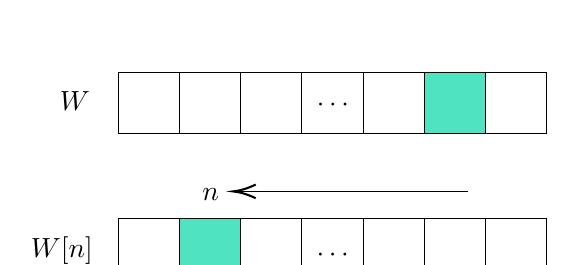
\begin{tikzpicture}[x=0.75pt,y=0.75pt,yscale=-1,xscale=1]
%uncomment if require: \path (0,300); %set diagram left start at 0, and has height of 300

%Shape: Square [id:dp0812615772659322] 
\draw   (130.67,41.72) -- (160.17,41.72) -- (160.17,71.22) -- (130.67,71.22) -- cycle ;
%Shape: Square [id:dp9156482978414704] 
\draw   (160.17,41.72) -- (189.67,41.72) -- (189.67,71.22) -- (160.17,71.22) -- cycle ;
%Shape: Square [id:dp8589697057894725] 
\draw   (189.67,41.72) -- (219.17,41.72) -- (219.17,71.22) -- (189.67,71.22) -- cycle ;
%Shape: Square [id:dp5527310059356019] 
\draw   (219.17,41.72) -- (248.67,41.72) -- (248.67,71.22) -- (219.17,71.22) -- cycle ;
%Shape: Square [id:dp3340966716018581] 
\draw   (248.67,41.72) -- (278.17,41.72) -- (278.17,71.22) -- (248.67,71.22) -- cycle ;
%Shape: Square [id:dp1473977553017456] 
\draw  [fill={rgb, 255:red, 80; green, 227; blue, 194 }  ,fill opacity=1 ] (278.17,41.72) -- (307.67,41.72) -- (307.67,71.22) -- (278.17,71.22) -- cycle ;
%Shape: Square [id:dp06348149501159495] 
\draw   (307.67,41.72) -- (337.17,41.72) -- (337.17,71.22) -- (307.67,71.22) -- cycle ;
%Shape: Square [id:dp4355149690645379] 
\draw   (130.67,112.22) -- (160.17,112.22) -- (160.17,141.72) -- (130.67,141.72) -- cycle ;
%Shape: Square [id:dp24955859820800752] 
\draw  [fill={rgb, 255:red, 80; green, 227; blue, 194 }  ,fill opacity=1 ] (160.17,112.22) -- (189.67,112.22) -- (189.67,141.72) -- (160.17,141.72) -- cycle ;
%Shape: Square [id:dp7712136013152768] 
\draw   (189.67,112.22) -- (219.17,112.22) -- (219.17,141.72) -- (189.67,141.72) -- cycle ;
%Shape: Square [id:dp13940177538276122] 
\draw   (219.17,112.22) -- (248.67,112.22) -- (248.67,141.72) -- (219.17,141.72) -- cycle ;
%Shape: Square [id:dp4166608510635037] 
\draw   (248.67,112.22) -- (278.17,112.22) -- (278.17,141.72) -- (248.67,141.72) -- cycle ;
%Shape: Square [id:dp6958291315519955] 
\draw   (278.17,112.22) -- (307.67,112.22) -- (307.67,141.72) -- (278.17,141.72) -- cycle ;
%Shape: Square [id:dp3744108591086348] 
\draw   (307.67,112.22) -- (337.17,112.22) -- (337.17,141.72) -- (307.67,141.72) -- cycle ;
%Straight Lines [id:da8996678375365978] 
\draw    (299,99) -- (188,99) ;
\draw [shift={(186,99)}, rotate = 360] [color={rgb, 255:red, 0; green, 0; blue, 0 }  ][line width=0.75]    (10.93,-3.29) .. controls (6.95,-1.4) and (3.31,-0.3) .. (0,0) .. controls (3.31,0.3) and (6.95,1.4) .. (10.93,3.29)   ;

% Text Node
\draw (101.33,49.62) node [anchor=north west][inner sep=0.75pt]    {$W$};
% Text Node
\draw (87.33,119.62) node [anchor=north west][inner sep=0.75pt]    {$W[n]$};
% Text Node
\draw (170,96.5) node [anchor=north west][inner sep=0.75pt]    {$n$};
% Text Node
\draw (225,53.5) node [anchor=north west][inner sep=0.75pt]  [rotate=-359.39]  {$\cdots $};
% Text Node
\draw (225,125.5) node [anchor=north west][inner sep=0.75pt]    {$\cdots $};

\end{tikzpicture}
\end{figure}
    
    \item $W^\vee$ denotes the linear dual with 
    \bea W^\vee_m=\on{Hom}(W_{-m},\mathbf{k}) \quad \text{for base field } \mathbf{k}. \eea
    
    \item Given two $\bZ$-graded vector spaces $V$, $W$, with base field being implicit,
    \bea \lb V\otimes W\rb_n &=\bigoplus_{i+j=n} \lb V_i\otimes W_j\rb,\\
    \on{Hom}(V,W)_n
    &= \bigoplus_i \on{Hom}(V_i, W_{i+n}).\eea
    
    \item $\sym^m(V)$ denotes a $m$-th graded symmetric tensor, which is $V^{\otimes m}/\sim$ where $a\otimes b\sim +(-1)^{|a||b|}b\otimes a$ (here $|a|$ is the parity of $a$).
    
    \item $\asym^m(V)$ denotes a $m$-th graded skew-symmetric tensor, which is $V^{\otimes m}/\sim$ where $a\otimes b\sim -(-1)^{|a||b|} b\otimes a$.

    \item We will write 
    $\sym(V)=\bigoplus_{m\geq 0} \sym^m(V)$ as the (graded) polynomial ring generated by $V$ and  $\widehat{\sym}(V)=\prod_{m\geq 0} \sym^m(V)$ as the (graded) formal power series ring generated by $V$.
\end{itemize}

\begin{prop}We have $\asym^k(V[1])\simeq \sym^k(V)[k]$.
\end{prop}
\begin{proof}
A very helpful exercise for the reader.
\end{proof}


\subsection*{CE complex for DGLA}
Let $(g,d,[-,-])$ be a DGLA. Let
\bea C^\blt(\fg)\coloneqq \sym^\blt(\fg^\vee[-1]).\eea
Since $\fg^\vee[-1]= \lb \fg[1]\rb^\vee$, $\sym^\blt \lb\fg^\vee[-1]\rb = \sym^\blt\lb \fg[1]\rb^\vee$, we can think of $C^\blt(\fg)$ as a (polynomial) function on $\fg[1]$. 
When $\fg$ is a Lie algebra,
\bea C^k(\fg)= \sym^k\lb \fg^\vee[-1]\rb\simeq \asym^k \fg^\vee[-k].\eea
This is $\asym^k \fg^\vee$ sitting at degree $k$. We get the usual CE.

Let 
\bea d_\fg: \fg^\vee[-1]\to \fg^\vee[-1]\eea
be the dual of $d:\fg \to \fg$ and \bea d_{[-,-]}:\fg^\vee[-1]\to \sym^2(\fg^\vee[-1])\simeq \asym^2 \fg^\vee[-2]\eea
be the dual of the bracket $[-,-]: \asym^2 \fg \to\fg$. Note that both $d_\fg$ and $d_{[-,-]}$ have $\on{deg}=1$ (check!).

Since $C^\blt(\fg)$ is freely generated by $\fg^\vee[-1]$, we can extend $d_\fg$ and $d_{[-,-]}$ to $C^\blt(\fg)$ by requiring them to
\begin{itemize}
    \item act on the generator $\fg^\vee[-1]$, as defined above,
    \item satisfy the graded Leibniz rule.
\end{itemize}

Define the \textbf{CE differential}
\bea d_{\on{CE}} \coloneqq d_\fg +d_{[-,-]}.\eea

\begin{clm}
$d_{\on{CE}}^2=0$.
\end{clm}
\begin{sproof}
We illustrate why this is true and leave the details to readers. In fact, if we represent

\bea
d_{\on{CE}}: \begin{fmffile}{dce1a}
    \begin{tabular}{c}
        \begin{fmfgraph*}(100,60)
                \fmfleft{i}
                \fmfright{o}
                \fmf{fermion,label=$d$,l.side=left,tension=4}{i,o}
        \end{fmfgraph*}
        \end{tabular}
    \end{fmffile}
    ~~~ + ~~~
    \begin{fmffile}{dce1b}
    \begin{tabular}{c}
        \begin{fmfgraph*}(100,60)
                \fmfleft{i1,i2}
                \fmfright{o}
                \fmf{fermion,tension=4}{i1,v}
                \fmf{fermion,tension=4}{i2,v}
                \fmf{fermion,tension=4}{v,o}
                \fmfv{label=$[-,,-]$,l.angle=45,decor.shape=circle,decor.filled=full,decor.size=2thick}{v}
        \end{fmfgraph*}
        \end{tabular}
    \end{fmffile},
\eea
then
\bea
d_{\on{CE}}^2: &
\begin{fmffile}{dce2a}
    \begin{tabular}{c}
        \begin{fmfgraph*}(100,50)
                \fmfleft{i}
                \fmfright{o}
                \fmf{fermion,label=$d^2$,l.side=left,tension=4}{i,o}
        \end{fmfgraph*}
        \end{tabular}
    \end{fmffile}
    \\ ~~~ & + ~~~
    \begin{fmffile}{dce2b}
    \begin{tabular}{c}
        \begin{fmfgraph*}(100,60)
                \fmfleft{i1,i2}
                \fmfright{o}
                \fmf{fermion,label=$d$,l.side=left,tension=4}{i2,v}
                \fmf{fermion,tension=4}{i1,v}
                \fmf{fermion,tension=5}{v,o}
                \fmfv{decor.shape=circle,decor.filled=full,decor.size=2thick}{v}
        \end{fmfgraph*}
        \end{tabular}
    \end{fmffile}
    ~~~ + ~~~
    \begin{fmffile}{dce2c}
    \begin{tabular}{c}
        \begin{fmfgraph*}(100,60)
                \fmfleft{i1,i2}
                \fmfright{o}
                \fmf{fermion,tension=4}{i2,v}
                \fmf{fermion,label=$d$,l.side=right,tension=4}{i1,v}
                \fmf{fermion,tension=5}{v,o}
                \fmfv{decor.shape=circle,decor.filled=full,decor.size=2thick}{v}
        \end{fmfgraph*}
        \end{tabular}
    \end{fmffile}
    ~~~ + ~~~
    \begin{fmffile}{dce2d}
    \begin{tabular}{c}
        \begin{fmfgraph*}(100,60)
                \fmfleft{i1,i2}
                \fmfright{o}
                \fmf{fermion,tension=4}{i1,v}
                \fmf{fermion,tension=4}{i2,v}
                \fmf{fermion,label=$d$,l.side=left,tension=5}{v,o}
                \fmfv{decor.shape=circle,decor.filled=full,decor.size=2thick}{v}
        \end{fmfgraph*}
        \end{tabular}
    \end{fmffile}
    \\ ~~~ & + ~~~
    \sum_{\text{permutations}} \lb
    \begin{fmffile}{dce2e}
    \begin{tabular}{c}
        \begin{fmfgraph*}(120,80)
                \fmfleft{i1,i2,i3}
                \fmfright{o}
                \fmf{fermion,tension=1}{i1,v2}
                \fmf{fermion,tension=1}{i2,v1}
                \fmf{fermion,tension=1}{i3,v1}
                \fmf{fermion,tension=2}{v1,v2}
                \fmf{fermion,tension=2}{v2,o}
                \fmfv{label=$[-,,-]$,l.angle=65,decor.shape=circle,decor.filled=full,decor.size=2thick}{v1}
                \fmfv{label=$[-,,-]$,l.angle=65,decor.shape=circle,decor.filled=full,decor.size=2thick}{v2}
        \end{fmfgraph*}
        \end{tabular}
    \end{fmffile}\rb.
\eea

We can ``see'' that 
$d_{\on{CE}}^2=0$ is equivalent to the defining properties of DGLA:
\begin{itemize}
    \item $d^2=0$,
    \item Leibniz rule: $d\lsb-,-\rsb=\lsb d(-),-\rsb\pm \lsb -,d(-)\rsb$,
    \item Jacobi identity.
\end{itemize}
$\lb C^\blt(\fg),d_{\on{CE}}\rb$ is called the \textbf{CE complex}.
\end{sproof}


\subsection*{Homotopy Lie algebra ($L_\infty$-algebra)}
Given a graded vector space $V$, we consider a (graded) derivation 
on $\sym(V)$:
\bea \delta: \sym(V) \to \sym(V),\eea
which satisfies the graded Leibniz rule
\bea \delta(a\otimes b)=(\delta a)\otimes b \pm a\otimes \delta b.\eea 
Such $\delta$ is completely determined by how $\delta$ acts on the generator
\bea \delta: V\to \sym(V).\eea

We can decompose
\bea \delta=\delta_0+\delta_1+\delta_2+\cdots,\eea
where $\delta_k:V\to \sym^k(V).$
For DGLA, we have $d_{\on{CE}}$ acting on $C^\blt(\fg)=\sym(\fg^\vee\lsb -1\rsb)$, where \bea d_{\on{CE}}=d_\fg+d_{[-,-]} =\delta_1+\delta_2.\eea
This is a derivation where only $\delta_1$, $\delta_2$ are nontrivial. It is natural to generalize this operator by encoding all possible components $\delta_k$. This leads to the \emph{$L_\infty$-algebra}.


\begin{defn}
An \textbf{$L_\infty$-algebra} is a $\bZ$-graded vector space $\fg$ with a collection of multilinear maps
\bea \ell_n: \asym^n \fg \to \fg, \quad \on{deg}(\ell_n)=2-n \quad (n\geq 1)\eea
satisfying the following $L_\infty$-relation
\bea \sum_{k=1}^n \pm \ell_{n-k+1}\lb \ell_k\lb \cdots\rb, \cdots\rb=0 \quad \forall n.\eea
\end{defn}
 
The complicated $L_\infty$-relation can be understood as follows. Let
\bea \delta_n: \fg^\vee\lsb-1\rsb \to \sym^n\lb \fg^\vee\lsb-1\rsb\rb\simeq \asym^n \fg^\vee \lsb-n\rsb\eea
denotes the dual of $\ell_n:\asym^n \fg\to\fg$. Note that
\bea \on{deg}(\ell_n)=2-n \ \LRA\ \on{deg}(\delta_n)=1.\eea
Let $\delta=\sum_{n\geq 1}\delta_n= \delta_1+\delta_2+\cdots$ defines a derivation on $C^\blt(\fg)=\widehat{\sym}\lb \fg^\vee\lsb -1\rsb\rb$ via the graded Leibniz rule. (Here we use the (graded) formal power series ring $\widehat{\sym}\lb \fg^\vee\lsb -1\rsb\rb$ so that $\delta$ is defined.) Then
\bea L_\infty \text{-relations for } \lcb \ell_n\rcb_{n\geq 1}\ \LRA\ \delta^2=0.\eea
$\lb C^\blt(\fg),\delta\rb$ is the CE complex for $\fg$.

If we represent each $\delta_n$ as a graph
\bea
n\lcb ~~~
    \begin{fmffile}{dce3}
    \begin{tabular}{c}
        \begin{fmfgraph*}(150,120)
                \fmfleft{i1,i2,i3,i4,i5,i6,i7,i8,i9,i10}
                \fmfright{o}
                \fmf{fermion,tension=1}{i10,v}
                \fmf{phantom,tension=1}{i9,v}
                \fmf{fermion,tension=1}{i8,v}
                \fmf{phantom,tension=1}{i7,v}
                \fmf{phantom,tension=1}{i6,v}
                \fmf{phantom,tension=1}{i5,v}
                \fmf{phantom,label=$\cdot$,l.side=left,tension=1}{i4,v}
                \fmf{phantom,label=$\cdot$,l.side=left,tension=1}{i3,v}
                \fmf{phantom,label=$\cdot$,l.side=left,tension=1}{i2,v}
                \fmf{fermion,tension=1}{i1,v}
                \fmf{fermion,tension=5}{v,o}
                \fmfv{label=$\ell_n$,label.angle=45,decor.shape=circle,decor.filled=full,decor.size=2thick}{v}
        \end{fmfgraph*}
        \end{tabular}
    \end{fmffile}
    \right.,
\eea
then $\delta^2=0$ can be pictured as 
\bea \sum_{\text{permutations}}\lb
    \begin{fmffile}{dce4}
        \begin{tabular}{c}
        \begin{fmfgraph*}(200,150)
                \fmfleft{h1,h2,h3,h4,h5,h6,h7,h8,h9,h10,i1,i2,i3,i4,i5,i6,i7,i8,i9,i10,i11,i12}
                \fmfright{o}
                \fmf{fermion,tension=1}{i12,v}
                \fmf{phantom,tension=1}{i11,v}
                \fmf{phantom,tension=1}{i10,v}
                \fmf{fermion,tension=1}{i9,v}
                \fmf{phantom,tension=1}{i8,v}
                \fmf{phantom,tension=1}{i7,v}
                \fmf{phantom,tension=1}{i6,v}
                \fmf{phantom,tension=1}{i5,v}
                \fmf{phantom,label=$\cdot$,l.side=left,tension=1}{i4,v}
                \fmf{phantom,label=$\cdot$,l.side=left,tension=1}{i3,v}
                \fmf{phantom,label=$\cdot$,l.side=left,tension=1}{i2,v}
                \fmf{fermion,tension=1}{i1,v}
                
                \fmf{fermion,tension=10}{h10,w}
                \fmf{phantom,tension=10}{h9,w}
                \fmf{phantom,tension=10}{h8,w}
                \fmf{phantom,tension=10}{h7,w}
                \fmf{phantom,tension=10}{h6,w}
                \fmf{phantom,tension=10}{h5,w}
                \fmf{phantom,label=$\cdot$,l.side=left,tension=10}{h4,w}
                \fmf{phantom,label=$\cdot$,l.side=left,tension=10}{h3,w}
                \fmf{phantom,label=$\cdot$,l.side=left,tension=10}{h2,w}
                \fmf{fermion,tension=10}{h1,w}
                
                \fmf{fermion,tension=10}{v,w}
                \fmf{fermion,tension=150}{w,o}
                \fmfv{label=$\ell_n$,label.angle=60,decor.shape=circle,decor.filled=full,decor.size=2thick}{v}
                \fmfv{label=$\ell_n$,label.angle=60,decor.shape=circle,decor.filled=full,decor.size=2thick}{w}
        \end{fmfgraph*}
        \end{tabular}
    \end{fmffile}
    \rb=0.
\eea

As we will see, this has a natural interpretation via Feynman diagram technique.

\noindent \textsc{References}:
\cite{Lada:2021vvm} and its references for a nice review on $L_\infty$-algebra and its relation in QFT,
\cite{Li:2018rnc} for a self-contained review on $L_\infty$-algebra which we are following in this lecture.

\section{Effective BV quantization}\label{sec:bv}
In the \nameref{sec:hla}, we discussed that
\bea \text{homotopy Lie algebra } (L_\infty-\text{algebra})\ \fg \LRA
\text{vector field } \delta \text{ on } \fg\lsb 1\rsb \text{ such that } \delta^2=0.\eea
We can write $\delta= \delta_1+\delta_2+\cdots$ where 
\bea \delta_k: \fg^\vee\lsb-1\rsb \to \sym^k\lb \fg^\vee\lsb-1\rsb\rb.\eea
For Lie algebra, $\delta=\delta_2$; for DGLA, $\delta=\delta_1+\delta_2$. 

\begin{conv}
Given $A,B\in \on{Hom}(V,V)$, we write
the \textbf{commutator} 
\bea \lsb A,B\rsb\coloneqq AB-(-1)^{|A||B|}BA,\eea
where $|A|$ is the degree of $A$. In particular, $\lsb A,B\rsb=AB+BA$ if $A,B$ are odd operators.
\end{conv}

\subsection*{BV master equation}
\begin{defn}
A \textbf{differential graded Batalin-Vilkovisky (DGBV) algebra} is a triple $\lb \cA,Q,\Delta\rb$ where
\bi[(1)]
\item $\cA$ is a graded commutative associative algebra,
\item $Q:\cA\to \cA$ is a derivation of $\on{deg} Q=1$ with $Q^2=0$,
\item $\Delta: \cA \to \cA$ is the BV operator, which is a second-order operator of $\on{deg}=1$ with $\Delta^2=0$,
\item $\lsb Q,\Delta\rsb=Q\Delta+\Delta Q=0.$
\ei
\end{defn}
Here $\Delta$ being \emph{second-order} means the following. Define the \textbf{BV bracket}
\bea \lcb a,b\rcb\coloneqq \Delta(ab)-(\Delta a)b-(-1)^{|a|} a\Delta b\quad \forall a,b\in \cA,\eea
which indicates the failure of $\Delta$ being a derivation. Then $\lcb -,-\rcb: \cA\otimes \cA\to \cA$ is a $\on{deg}=1$ operator satisfying
\bi[(1)]
\item $\lcb a,b\rcb= (-1)^{|a||b|}\lcb b,a\rcb$,
\item $\lcb a,bc\rcb=\lcb a,b\rcb c+(-1)^{\lb|a|+1\rb |b|} b\lcb a,c\rcb$,
\item $\Delta \lcb a,b\rcb=-\lcb \Delta a,b\rcb-(-1)^{|a|} \lcb a, \Delta b\rcb$.
\ei

\begin{eg}
Let $X$ be a smooth manifold and $\Omega$ be a volume form on $X$. Then we have the 
$\lb \on{PV}^\blt (X),\Delta_\Omega\rb$ complex, where $\Delta_\Omega: \on{PV}^{k}\to \on{PV}^{k-1}$ is the BV operator (or the divergence operator with respect to $\Omega$). Define $\lcb \alpha,\beta\rcb\coloneqq \Delta_\Omega\lb \alpha\beta\rb- \lb\Delta_\Omega \alpha\rb \beta-(-1)^{|\alpha|}\alpha\Delta_\Omega\beta$. Then $\lcb -,-\rcb$ is the \textbf{Schouten-Nijenhuis bracket} (up to a sign).
\end{eg}

\begin{fact}
$\lcb -,-\rcb$ does not depend on the choice of $\Omega$.
\end{fact}

\begin{eg}
Let $X$ be a Calabi-Yau manifold and $\Omega$ be a holomorphic volume form. The polyvector field is
\bea \on{PV}^{k,l}(X)=\Omega^{0,l} \lb X,\asym^k T_X^{1,0}\rb,\eea
the Dolbeault differential operator is 
\bea \pb: \on{PV}^{k,l}\to \on{PV}^{k,l+1},\eea
the BV operator (i.e. the divergence operator with respect to $\Omega$) is
\bea \Delta: \on{PV}^{k,l}\to \on{PV}^{k-1,l}.\eea
Then $\lb \on{PV}^{-\blt,\blt}(X), \pb, \Delta\rb$ is a DGBV.
\end{eg}

\begin{rmk}
The existence of such structure implies that the local moduli of complex structure of the Calabi-Yau manifold $X$ is smooth. This follows from the Bogomolov-Tian-Todorov (BTT) lemma.
\end{rmk}

\begin{defn}
Let $\lb \cA,Q,\Delta\rb$ be a DGBV. Suppose an element $I_0\in \cA_0$, where $\on{deg}(I_0)=0$. $I_0$ is said to satisfy \textbf{classical master equation (CME)} if  
\bea QI_0+\hf \lcb I_0,I_0\rcb=0.\eea
This implies $\lb Q+\lcb I_0,-\rcb\rb^2=0$ on $\cA$.
In good situation, we can write
\bea  Q+\lcb I_0,-\rcb=\lcb S_0,-\rcb,\eea
where $S_0$ is the classical action and $I_0$ is its interaction part. 
Then the CME means $\lcb S_0, S_0\rcb=0$.
\end{defn}

The upshot here is that any classical action along with gauge symmetry leads to a solution of CME.

\begin{defn}
$I\in \cA_0\llb \hbar\rrb$ is said to satisfy the \textbf{quantum master equation (QME)} if 
\bea QI+ \hbar \Delta I+\hf \lcb I,I\rcb =0.\eea
We can write $I=I_0+\hbar I_1+\hbar^2 I_2+\cdots$. When $\hbar\to 0$, the above equation reduces to 
\bea QI_0+\hf \lcb I_0,I_0\rcb=0. \eea
In good situation (in QFT), we write
\bea  Q+\lcb I,-\rcb=\lcb S,-\rcb,\eea
where $S$ is the quantum action.
Then the QME means $\hbar \Delta S+\hf \lcb S, S\rcb=0$.
\end{defn}
In QFT, the quantization process asks the classical action $S_0$ solving the CME to be quantized to the quantum action $S=S_0+\hbar S_1+\hbar^2 S_2+\cdots$ solving the QME.

\begin{eg}
QME $\LRA (Q+\hbar \Delta) e^{I/\hbar}=0$
(or in good situation $\Delta e^{S/\hbar}=0$).
\end{eg}

\paragraph{Toy model: (-1)-shifted symplectic geometry.}
Let $(V, Q,\omega)$ be a finite dimensional differential graded symplectic space.
\begin{itemize}
    \item $Q: V\to V$ is the differential operator with $Q^2=0$, 
    \item $\omega: \asym^2 V\to \bR$ or $\bC$ is a non-degenerate pairing of $\on{deg}=-1$, or explicitly $\omega(a,b)=0$ unless $|a|+|b|=1$,
    \item $Q(\omega)=0$, or explicitly  $\omega(Q(a),b)+(-1)^a\omega(a, Q(b))=0$.
\end{itemize}
The \emph{non-degeneracy} of $\omega$ implies an isomorphism
\bea \omega: V^\vee \xrightarrow{\ \sim\ } V\lsb 1\rsb. \eea
This allows us to identify
\bea \asym^2 V^\vee \xleftrightarrow{\ \sim\ } \asym^2 \lb V[1]\rb \simeq \sym^2(V)[2], \qquad \omega\in \asym^2 V^\vee \xleftrightarrow{\ \sim\ } K[2],\eea
where $K=\omega^{-1}\in \sym^2(V)$ is the \textbf{Poisson kernel} with $\on{deg} K=1$ and $Q(K)=0$.
We obtain a DGBV $\lb \cA,Q,\Delta_K\rb$ as follows. 
\begin{itemize}
    \item $\cA=\sO(V)=\widehat{\sym}(V^\vee)$ is a space of formal functions on $V$,
    \item $Q:\cA\to\cA$ is the differential induced from $Q:V\to V$,
    \item $\Delta_K: \sym^m (V^\vee)\to \sym^{m-2} (V^\vee)$ is the contraction with the Poisson kernel $K\in \sym^2(V)$. Explicitly, for $\alpha_i\in V^\vee$, 
    \bea \Delta_K(\alpha_1\otimes\cdots \otimes\alpha_m)=\sum_{i<j}\pm \lan K,\alpha_i\otimes \alpha_j\ran \alpha_1\otimes \cdots \otimes \widehat{\alpha_i} \otimes \cdots \otimes \widehat{\alpha_j} \otimes \cdots \otimes \alpha_m.\eea
    Here $\pm$ is the \emph{Koszul sign} by permuting graded objects.
\end{itemize}

\begin{prop}
$(\sO(V),Q,\Delta_K)$ is a DGBV.
\end{prop}
\begin{proof}
Exercise.
\end{proof}

Let $S_0\in \sO(V)$ solve the CME:
\bea \lcb S_0,S_0\rcb=0 \quad (\on{deg} S_0=0).
\eea
Then $\delta=\lcb S_0,-\rcb$ defines a vector field on $V$ with $\on{deg} \delta=1, \delta^2=0$. Hence $(\fg=V[-1], \delta)$ is an $L_\infty$-algebra.

\subsection*{Field theory via BV formalism}
A classical field theory can be usually organized into an $\infty$-dimensional $(-1)$-symplectic geometry $(\cE,Q,\omega)$ where
\bi[(1)]
\item $\cE=\Gamma\lb X,E^\blt\rb$ is the space of fields (or space of sections), where $E^\blt$ is the graded vector bundle,
\item $(\cE,Q)$ is an elliptic complex, in which the differential $Q$ is naturally defined as follows.
\bea \cdots \longrightarrow \cE^{-1}\xrightarrow{\ Q\ }\cE^0 \xrightarrow{\ Q\ }\cE^1 \longrightarrow\cdots.\eea
$Q$ is an elliptic operator. For example, $Q$ can be the de Rham differential $d$ or the Dolbeault differential $\pb$.
\item $\omega$ is the local $(-1)$-symplectic pairing, where
\bea \omega(\alpha,\beta)= \int_X \lan \alpha,\beta\ran \quad \forall \alpha,\beta\in\cE\eea
and is compatible with $Q$:
\bea \omega(Q(\alpha),\beta)+(-1)^\alpha \omega(\alpha,Q(\beta))=0.\eea
\ei

To describe the quantization, we perform the \emph{toy model}, in which we define
\begin{itemize}
    \item $\cE^\vee \coloneqq\on{Hom}_X(\cE,\bR)$ is a distribution on $X$,
    \item $(\cE^\vee)^{\otimes n}=\on{Hom}_{X^n}(\cE^{\otimes n},\bR)$ is a distribution on $X^n$,
\end{itemize}
so $\sym^n(\cE^\vee)$ is defined.
Let us form 
\bea \sO(\cE)\coloneqq \prod_{n\geq 0}\sym^n(\cE^\vee).\eea
Let $\sO_{loc}(\cE)\subset \sO(\cE)$ be a \textbf{space of local functionals}, which contains the set 
\bea\lcb \left. \int_X \cL\ \right|\ \cL \text{ is the Lagrangian density} \rcb.\eea
The Poisson kernel is $K=\omega^{-1}=$``$\lb \int_X \lan \alpha,\beta\ran\rb^{-1}$'', which is a $\delta$-function distribution as in $f(x)=\int dy \delta_{x,y} f(y) $. $K$ is a \textbf{distributional section} of $\sym^2(\cE)$.

However, there is one problem. The action of $\Delta_K$ on $\sO(\cE)$ ($\Delta_K \curvearrowright\sO(\cE)$) is ill-defined since it is a pairing of two distributions, each of which is in infinite-dimensional space, leading to $\infty$. This is the famous \textbf{ultraviolet problem}.

\begin{eg}
In classical sense, the corresponding BV bracket $\lcb -,-\rcb$ is well-defined on local functionals $\sO_{loc}(\cE)$:
\bea \lcb -,-\rcb: \sO_{loc}(\cE)\times \sO_{loc}(\cE)\to \sO_{loc}(\cE).\eea
\bea
    \begin{fmffile}{fdd}
    \begin{tabular}{c}
        \begin{fmfgraph*}(150,50)
                \fmfleft{i1,i2,i3}
                \fmfright{o1,o2,o3}
                \fmf{plain,tension=4}{i1,v1}
                \fmf{plain,tension=4}{i2,v1}
                \fmf{plain,tension=4}{i3,v1}
                \fmf{plain,tension=4}{v2,o1}
                \fmf{plain,tension=4}{v2,o2}
                \fmf{plain,tension=4}{v2,o3}
                \fmf{plain,label=$\delta_{x,,y}$,label.side=left,tension=4}{v1,v2}
                \fmfv{label=$\int_X\cL_1$,label.angle=-60,decor.shape=circle,decor.filled=full,decor.size=2thick}{v1}
                \fmfv{label=$\int_X\cL_2$,label.angle=-120,decor.shape=circle,decor.filled=full,decor.size=2thick}{v2}
        \end{fmfgraph*}
        \end{tabular}
    \end{fmffile}
    ~~~ =\ \int_X \lb \cdots\rb.
\eea
Hence, CME makes sense for local functionals. But for quantization, $I_0\to I=I_0+\hbar I_1+\cdots$. We have
\bea QI+\hbar \Delta I+\hf \lcb I,I\rcb=0.\eea
The term $\hbar \Delta I$ is problematic and can be solved by the renormalization technique.
\end{eg}

\begin{eg}[Chern-Simons (CS) theory]
Let $X$ be a 3-manifold, $\fg$ be the Lie algebra, and $\Tr$ be the Killing pairing on $\fg$.
\begin{itemize}
    \item $\cE=\Omega^\blt\lb X,\fg[1]\rb$ where
        \begin{table}[!htpb]
            \centering
            \begin{tabular}{l|cccc}\toprule
            $\mathbf{\Omega^\blt}$ & $\Omega^0(X,\fg)$ & $\Omega^1(X,\fg)$ & $\Omega^2(X,\fg)$ & $\Omega^3(X,\fg)$\\ \hline
            \textbf{deg} & -1 & 0 & 1 & 2\\ \hline
            \textbf{name} & ghost & field (connection) & anti-field & anti-ghost\\ \bottomrule
            \end{tabular}\end{table}
        
    \item $\omega(\alpha,\beta)=\pm \int_X \Tr \lan \alpha,\beta\ran, \quad \on{deg}\omega=-1$,
    \item The CS action functional is 
    \bea\on{CS}[\cA]=\int \Tr\lb \hf \cA\wedge d\cA+\frac{1}{6}\cA\wedge [\cA,\cA]\rb,\eea 
    where the first term is the free part of the action and the second term is the interaction part, $I$. Here the master field is \bea\cA=c+A+A^\vee+c^\vee=\Omega^0+\Omega^1+\Omega^2+\Omega^3 \in \cE.\eea
    Hence,
    \bea\on{CS}[\cA]=\int \Tr\lb \hf A\wedge dA+\frac{1}{6}A\wedge [A,A]\rb+ \text{terms containing ghosts},\eea 
\end{itemize}

\begin{clm}
$\on{CS}[\cA]$ satisfies the CME: $\lcb \on{CS}, \on{CS}\rcb=0$.
\end{clm}
If we write $\on{CS}=\text{free}+I$ as above, then $\lcb \text{free},-\rcb=d$. Hence,
$\text{CME}\LRA dI+\hf \lcb I,I\rcb=0$.
One way to see this is that $\Omega^\blt(X,\fg)$ is a DGLA $\RA$ CME.
\end{eg}

\subsection*{Costello's homotopic renormalization}
We have seen that the action
\bea
\Delta_K \curvearrowright \sO(\cE)
\eea
is ill-defined naively, in which $K=\omega^{-1}$ is singular.

\paragraph{Toy model.} 
Let $(V,Q)$ be a finite dimensional complex and $K_0\in \sym^2(V)$ be the Poisson kernel with $\on{deg} K_0=1$ and $Q(K_0)=0$. Then $\Delta_0: \sO(V)\to \sO(V)$ is a BV operator by contracting with $K_0$. Let $P\in \sym^2(V)$, $\on{deg} P=0$. Consider the \emph{chain homotopy} for BV kernel:
\bea K_P=K_0+Q(P)=K_0+(Q\otimes 1+1\otimes Q)P,\eea
then $\on{deg}(K_P)=1$, $Q(K_P)=QK_0+Q^2(P)=0$. We can consider a new BV operator
$\Delta_P$, which is a contraction with $K_P$.

\begin{prop}
$\lb Q+\hbar \Delta_P\rb e^{\hbar\p_P}=e^{\hbar\p_P}\lb Q+\hbar \Delta_0\rb$.
\end{prop}
Here $\p_P$ is the second order operator of contracting with $P\in \sym^2(V)$:
\bea \p_P: \sym^n(V^\vee)\to \sym^{n-2}(V^\vee).\eea
Then we have the commutative diagram
\bea
\begin{tikzcd}
\sO(V)\llb \hbar\rrb \ar[r, "e^{\hbar\p_P}"] \ar[d,"Q+\hbar \Delta_0"]
& \sO(V)\llb \hbar\rrb \ar[d,"Q+\hbar \Delta_P"] \\
\sO(V)\llb \hbar\rrb \ar[r, "e^{\hbar\p_P}"]
& \sO(V)\llb \hbar\rrb
\end{tikzcd}
\eea
which implies that
\bea \text{QME for } (\sO(V),Q,\Delta_0) \xrightarrow{e^{\hbar \p_P}}
\text{QME for } (\sO(V),Q,\Delta_P),\eea
where $e^{\hbar \p_P}$ is the homotopy RG flow. Hence,
\bea \lb Q+\hbar \Delta_0\rb e^{I/\hbar}=0 \LRA \lb Q+\hbar \Delta_P\rb e^{\Tilde{I}/\hbar}=0\eea
where $e^{\Tilde{I}/\hbar}=e^{\hbar \p_P}e^{I/\hbar}$.
As we have seen before, this can be expressed by the Feynman diagrams:
\bea \Tilde{I}=\sum_{\text{connected graph}}\lb 
    \begin{fmffile}{fddi}
    \begin{tabular}{c}
        \begin{fmfgraph*}(100,50)
                \fmfleft{i1,i2}
                \fmfright{o1,o2}
                \fmf{plain,tension=4}{i1,v1}
                \fmf{plain,tension=4}{i2,v1}
                \fmf{plain,tension=4}{v2,o1}
                \fmf{plain,tension=4}{v2,o2}
                \fmf{plain,left,label=$P$,label.side=left,tension=3}{v1,v2,v1}
                \fmfv{label=$I$,label.angle=170,decor.shape=circle,decor.filled=full,decor.size=2thick}{v1}
                \fmfv{label=$I$,label.angle=10,decor.shape=circle,decor.filled=full,decor.size=2thick}{v2}
        \end{fmfgraph*}
        \end{tabular}
    \end{fmffile}\rb.
\eea

\paragraph{Back to QFT.}
Consider the $\infty$-dimensional $(-1)$-symplectic geometry $(\cE=\Gamma(X,E^\blt),Q,\omega)$ with the $\delta$-function distribution $K_0=\omega^{-1}$ and $Q(K_0)=0$.

\noindent\emph{Costello's approach}: use the elliptic regularity:
\bea H^\blt(\text{distributions}, Q)=H^\blt(\text{smooth functions}, Q).\eea 
We can write $K_0=K_r+QP_r$, where $K_r$ is smooth and $P_r$ is singular, called the \emph{parametrix}. $\Delta_r:\sO(\cE)\to \sO(\cE)$ is the BV operator contracting with $K_r$, which is well-defined since $K_r$ is smooth. Hence $\lb \sO(\cE),Q,\Delta_r\rb$ is the ``effective'' DGBV.

Let $r'$ be another regularization such that
\bea K_0=K_{r'}+QP_{r'}.\eea
Hence we find a smooth kernel $P^{r'}_r$ from 
\bea K_{r'}-K_r=QP^{r'}_r.\eea
Let $\p_{P^{r'}_r}: \sO(\cE)\to \sO(\cE)$ be contracting with the smooth kernel $P^{r'}_r$. Hence, we have a homotopy RG flow:
\bea \lb\sO(\cE)\llb \hbar\rrb,Q+\hbar\Delta_r\rb \xrightarrow{\exp{\lb \hbar \p_{P^{r'}_r}\rb}}
\lb\sO(\cE)\llb \hbar\rrb,Q+\hbar\Delta_{r'}\rb.\eea

\begin{defn}[Costello]
An effective solution of perturbative BV quantization of $I_0$ (which solves CME) is given by a family $I[r]\in \sO(\cE)\llb \hbar\rrb$ (for each choice of regularization $P_r$) such that
\begin{itemize}
    \item $\lb Q+\hbar \Delta_r\rb e^{I[r]/\hbar}=0$ is the effective QME,
    \item $e^{I[r']/\hbar}=\exp{\lb \hbar \p_{P^{r'}_r}\rb} e^{I[r]/\hbar}$ is the homotopy RG flow, or equivalently,
    \bea I[r']=\sum_{\text{connected graph}}\lb 
    \begin{fmffile}{fddj}
    \begin{tabular}{c}
        \begin{fmfgraph*}(100,50)
                \fmfleft{i1,i2}
                \fmfright{o1,o2}
                \fmf{plain,tension=4}{i1,v1}
                \fmf{plain,tension=4}{i2,v1}
                \fmf{plain,tension=4}{v2,o1}
                \fmf{plain,tension=4}{v2,o2}
                \fmf{plain,left,label=$P$,label.side=left,tension=3}{v1,v2,v1}
                \fmfv{label=$I[r]\ $,label.angle=170,decor.shape=circle,decor.filled=full,decor.size=2thick}{v1}
                \fmfv{label=$I[r]$,label.angle=10,decor.shape=circle,decor.filled=full,decor.size=2thick}{v2}
        \end{fmfgraph*}
        \end{tabular}
    \end{fmffile}\rb,
\eea
\item $I[r]$ is asymptotic local when $r\to 0$ and $I_0=\lim_{r\to 0}\lim_{\hbar\to 0}I[r]$. 
\end{itemize}
\end{defn}

\noindent \textsc{References}:
\cite{costello2011renormalization} for Costello's homotopy renormalization theory, \cite{Li:2016gcb} for the style of the lecture.

\section{Quantization and obstruction}\label{sec:qo}
In the \nameref{sec:bv}, we want to find an $\infty$-dimensional $(-1)$-symplectic geometry $(\cE,Q,\omega)$ to describe the QFT.
We have the classical data: the space of \textbf{local functionals}, $\cO_{\text{loc}}(\cE)\subset \cO(\cE)$, in which the classical interaction $I_0=\int_X \cL$ is an element of $\cO_{\text{loc}}(\cE)$. $I_0$ solves the CME: $QI_0+\hf \lcb I_0,I_0\rcb_0=0$. Here $\lcb -,-\rcb_0$ is the BV bracket with respect to the BV kernel $K_0=\omega^{-1}$ and is well-defined on $\cO_{\text{loc}}(\cE)$. However the BV operator $\Delta_0$ is ill-defined on $\cO_{\text{loc}}(\cE)$ and $\cO(\cE)$, where the naive QME $QI_0+\hbar \Delta_0 I_0+\hf \lcb I_0,I_0\rcb=0$ does not make sense.

One way out of this problem is to use regularization to define an effective QME. We defined the Poisson kernel $K_0=K_r+QP_r$, leading to a well-defined BV operator $\Delta_r$ on $\cO(\cE)$. For each $r$, we construct $I[r]\in \cO(\cE)$ solving the effective QME:
\bea \lb Q+\hbar\Delta_r\rb e^{I[r]/\hbar}=0\eea
and different regularizations are related by the homotopy RG (HRG) flow:
\bea e^{I[r']/\hbar}=\exp{\lb \hbar \p_{P^{r'}_r}\rb} e^{I[r]/\hbar}.\eea
We have seen that the effective QME and the HRG are compatible.
\bea
\tikzset{every picture/.style={line width=0.75pt}} %set default line width to 0.75pt    
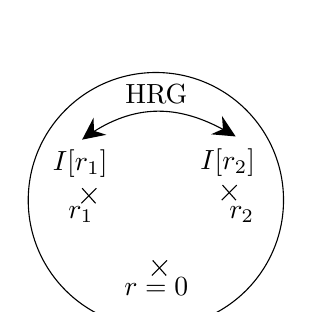
\begin{tikzpicture}[x=0.75pt,y=0.75pt,yscale=-1,xscale=1]
%uncomment if require: \path (0,300); %set diagram left start at 0, and has height of 300

%Shape: Circle [id:dp6926154379932559] 
\draw   (50,84.5) .. controls (50,50.53) and (77.53,23) .. (111.5,23) .. controls (145.47,23) and (173,50.53) .. (173,84.5) .. controls (173,118.47) and (145.47,146) .. (111.5,146) .. controls (77.53,146) and (50,118.47) .. (50,84.5) -- cycle ;
%Straight Lines [id:da2262569241568375] 
\draw    (75.98,78.77) -- (82.47,86.03) ;
%Straight Lines [id:da9042410789635242] 
\draw    (75.59,86.03) -- (82.85,78.77) ;

%Straight Lines [id:da7965197666945929] 
\draw    (143.59,77.24) -- (150.08,84.5) ;
%Straight Lines [id:da23412451653488264] 
\draw    (143.2,84.5) -- (150.46,77.24) ;

%Straight Lines [id:da694164688117211] 
\draw    (109.97,113.53) -- (116.47,120.79) ;
%Straight Lines [id:da27199650302361067] 
\draw    (109.59,120.79) -- (116.85,113.53) ;

%Curve Lines [id:da21026083909699889] 
\draw    (78.71,53.37) .. controls (106.69,33.96) and (129.65,42.23) .. (147.47,52.37) ;
\draw [shift={(149.95,53.81)}, rotate = 210.62] [fill={rgb, 255:red, 0; green, 0; blue, 0 }  ][line width=0.08]  [draw opacity=0] (10.72,-5.15) -- (0,0) -- (10.72,5.15) -- (7.12,0) -- cycle    ;
\draw [shift={(75.98,55.34)}, rotate = 323.13] [fill={rgb, 255:red, 0; green, 0; blue, 0 }  ][line width=0.08]  [draw opacity=0] (10.72,-5.15) -- (0,0) -- (10.72,5.15) -- (7.12,0) -- cycle    ;

% Text Node
\draw (68.07,86.16) node [anchor=north west][inner sep=0.75pt]    {$r_{1}$};
% Text Node
\draw (145.59,86.16) node [anchor=north west][inner sep=0.75pt]    {$r_{2}$};
% Text Node
\draw (95.02,120.54) node [anchor=north west][inner sep=0.75pt]    {$r=0$};
% Text Node
\draw (60.62,58.71) node [anchor=north west][inner sep=0.75pt]    {$I[r_{1}]$};
% Text Node
\draw (131.67,58.33) node [anchor=north west][inner sep=0.75pt]    {$I[r_{2}]$};
% Text Node
\draw (95.53,27.36) node [anchor=north west][inner sep=0.75pt]   [align=left] {HRG};
\end{tikzpicture}
\eea


\subsection*{Heat kernel regularization}
Typically, fixing a choice of metric, we have 
\begin{itemize}
    \item the adjoint of $Q:\cE\to \cE$, denoted as $Q^\dagger: \cE\to \cE$,
    \item a generalized Laplacian, $\lsb Q,Q^\dagger\rsb= QQ^\dagger+Q^\dagger Q$ 
\end{itemize}
Hence we can define a heat operator $e^{-L\lsb Q,Q^\dagger\rsb}$ for $L>0$. Let $K_L\in \sym^2(\cE)$ be the kernel of the heat operator by 
\bea \lb e^{-L\lsb Q,Q^\dagger\rsb}\alpha\rb \lb x\rb
=\int dy \lan K_L(x,y),\alpha(y)\ran\quad \text{for }\alpha\in\cE.\eea 
Here $\lan-,-\ran$ is the pairing from $\omega$. Note that
\begin{itemize}
    \item $K_0=\lim_{L\to 0} K_L$ is the $\delta$-function distribution $\omega^{-1}$,
    \item $K_L\in \sym^2(\cE)$ is smooth for $L>0$.
\end{itemize}

Let $P_L$ be the kernel of the operator $\int_0^L dt\ Q^\dagger e^{-t\lsb Q,Q^\dagger\rsb} $. Explicitly, we have 
\bea P_L= \int_0^L dt \lb Q^\dagger \otimes 1\rb K_t.\eea
The operator equation 
\bea \lsb Q, \int_0^L dt\ Q^\dagger e^{-t\lsb Q,Q^\dagger\rsb} \rsb 
= \int_0^L dt \lsb Q,Q^\dagger\rsb e^{-t\lsb Q,Q^\dagger\rsb} 
=1=e^{-L\lsb Q,Q^\dagger\rsb}.\eea
This is translated into the kernel equation:
\bea K_0-K_L=(Q\otimes 1+1\otimes Q)P_L\eea
or simply written as
\bea K_0-K_L=QP_L.\eea

We can use $K_L$ to define the effective QME. For $0<\vep<L$, similarly the operator equation is 
\bea \lsb Q, \int_\vep^L dt\ Q^\dagger e^{-t\lsb Q,Q^\dagger\rsb} \rsb 
=e^{-\vep\lsb Q,Q^\dagger\rsb}-e^{-L\lsb Q,Q^\dagger\rsb}\eea
or 
\bea K_\vep-K_L=(Q\otimes 1+1\otimes Q)P_\vep^L,\eea
where $P^L_\vep= \int_\vep^L dt \lb Q^\dagger \otimes 1\rb K_t$ is called the {\em regularized propagator}. Now we can use $P^L_\vep$ to connect the effective QME at $\vep$ with the effective QME at $L$ via the homotopy RG, $\exp{\lb \hbar\p_{P_\vep^L}\rb}$.

\subsection*{Constructing effective BV quantization using heat kernel regularization}
\paragraph{Step 1: The method of counter-term.}
Let $I_0\in \cO_{\text{loc}}(\cE)$ be the classical interaction. Since $P_0^L$ is singular, the limit $\lim_{\vep\to 0} \exp{\lb \hbar\p_{P_\vep^L}\rb} e^{I_0/\hbar}$ does not exist. Pictorially, all the loop diagrams, such as
\bea 
    \begin{fmffile}{fddlim}
    \begin{tabular}{c}
        \begin{fmfgraph*}(100,50)
                \fmfleft{i1,i2}
                \fmfright{o1,o2}
                \fmf{plain,tension=4}{i1,v1}
                \fmf{plain,tension=4}{i2,v1}
                \fmf{plain,tension=4}{v2,o1}
                \fmf{plain,tension=4}{v2,o2}
                \fmf{plain,left,label=$P_\vep^L$,label.side=left,tension=3}{v1,v2,v1}
                \fmfv{label=$I_0$,label.angle=170,decor.shape=circle,decor.filled=full,decor.size=2thick}{v1}
                \fmfv{label=$I_0$,label.angle=10,decor.shape=circle,decor.filled=full,decor.size=2thick}{v2}
        \end{fmfgraph*}
        \end{tabular}
    \end{fmffile}
\eea
are divergent as $\vep\to 0$.

We can find a {\em counter-term} $I^\eps\in \hbar \cO_{\text{loc}}(\cE)\llb \hbar\rrb$ which is $\vep$-dependent and is singular as $\vep\to 0$ such that
\bea \lim_{\vep\to 0} \exp{\lb \hbar\p_{P_\vep^L}\rb} e^{\lb I_0+I^\eps\rb/\hbar}\coloneqq e^{I[L]^{\text{naive}}/\hbar}\eea exists. 
Such defined $I[L]^{\text{naive}}$ has the following advantage for $0<L_1<L_2$, 
\bea e^{I[L_2]^{\text{naive}}/\hbar}
&= \lim_{\vep\to 0} \exp{\lb \hbar\p_{P_\vep^{L_2}}\rb} e^{\lb I_0+I^\eps\rb/\hbar}\\
&= \lim_{\vep\to 0} \exp{\lb \hbar\p_{P_{L_1}^{L_2}}\rb} \exp{\lb \hbar\p_{P_\vep^{L_1}}\rb} e^{\lb I_0+I^\eps\rb/\hbar} \quad \text{using } P_\vep^{L_2}=P_{L_1}^{L_2}+P_\vep^{L_1}\\
&= \exp{\lb \hbar\p_{P_{L_1}^{L_2}}\rb} \lim_{\vep\to 0} \exp{\lb \hbar\p_{P_\vep^{L_1}}\rb} e^{\lb I_0+I^\eps\rb/\hbar} \quad \text{since } P_{L_1}^{L_2} \text{ is smooth}\\
&= \exp{\lb \hbar\p_{P_{L_1}^{L_2}}\rb} e^{I[L_1]^{\text{naive}}/\hbar}.
\eea
In other words, the family $\lcb I[L_1]^{\text{naive}}\rcb_{L>0}$ satisfies the homotopy RG. However, $\lcb I[L_1]^{\text{naive}}\rcb_{L>0}$ may not satisfy the QME.

\paragraph{Step 2: Further corrections.}
Adjust $I^\eps$ to $\Tilde{I}^\eps$ by finding further corrections such that
\bea e^{I[L]/\hbar}
&= \lim_{\vep\to 0} \exp{\lb \hbar\p_{P_\vep^{L}}\rb} e^{\lb I_0+\Tilde{I}^\eps\rb/\hbar}.\eea
Then the defined limit $I[L]$ satisfies the QME.

\begin{rmk}
Step 1 is always possible.
Step 2 is NOT always possible; it might have {\em obstructions}, in physics this is called the {\em gauge anomaly}.
\end{rmk}

\begin{rmk}
There are cases where $\vep$-dependent counter-terms are not required in the sense that the limit 
\bea e^{I[L]/\hbar}
&= \lim_{\vep\to 0} \exp{\lb \hbar\p_{P_\vep^{L}}\rb} e^{I/\hbar}\eea
exists for a large class of local $I\in \cO_{\text{loc}}(\cE)\llb\hbar\rrb$. Such a theory is called \textbf{ultraviolet (UV)-finite}. Then we can explore the meaning of the effective QME $\lb Q=\hbar \Delta_L\rb e^{I[L]/\hbar}=0$ or $QI[L]+\hbar \Delta_L I[L]+\hf \lcb I[L],I[L]\rcb_L=0$. The upshot is that $L\to 0$ has a meaning in which the effective QME is reduced to $QI+\hf \lsb I,I\rsb=0$, where $\lsb-,-\rsb$ is the {\em quantum deformed bracket}.
\end{rmk}

We will explain two main UV-finite examples:
\bi[(1)]
\item Chern-Simons type topological theory.
\item In particular, we will discuss topological quantum mechanics (2d chiral theory).
\ei

\subsection*{Deformation-Obstruction theory}
Let's first consider the quantization problem CME $\leadsto$ QME in a DGBV $\lb \cA,Q,\Delta\rb$. Let $I_0\in \cA_0$ solve the CME $QI_0+\hf \lcb I_0,I_0\rcb=0$. Our goal is to find 
\bea I=I_0+I_1\hbar+I_2\hbar^2+\cdots \in \cA\llb \hbar\rrb\eea
solving the QME $QI+\hbar\Delta I+\hf \lcb I,I \rcb=0$.

\paragraph{Strategy:} find $I_1,I_2,\cdots$ in order of $\hbar$.
\bea QI+\hbar\Delta I+\hf \lcb I,I \rcb=\cO(\hbar^{n+1})\quad (n\geq 0).\eea 
\begin{itemize}
    \item $n=0$: this is the initial data of CME $QI_0+\hf \lcb I_0,I_0\rcb=0$.
    \item $n=1$: $\hbar$-term gives $QI_1+\Delta I_0+\lcb I_0,I_1 \rcb=0$. We need to find $I_1$ solving the above equation. Let us write it as 
    \bea QI_1+\lcb I_0,I_1 \rcb=\Delta I_0. \eea
    For convenience, let us denote $\delta=Q+\lcb I_0,-\rcb$. The CME implies that $\delta^2=0$. We need to solve 
    \bea \delta I_1=-\Delta I_0.\eea
    A key observation is that $\delta\lb -\Delta I_0\rb=0$ (exercise). So we see that $-\Delta I_0$ is $\delta$-closed. The solvability of $I_1$ asks whether $-\Delta I_0$ is $\delta$-exact. Let $\cO_1=\Delta I_0$ and let $\lsb \cO_1\rsb\in H^1(\cA,\delta)$ be the corresponding $\delta$-cohomology class. Then
    \begin{prop}
    $I_1$ can be solved $\LRA \lsb \cO_1\rsb=0$ in $H^1(\cA,\delta)$.
    \end{prop}
    Assume $\lsb \cO_1\rsb=0$. Let $I_1$ and $\Tilde{I}_1$ be two solutions. Then
    \bea \delta(I_1-\Tilde{I}_1)=0 \RA \Tilde{I}_1-I_1 \text{ is } \delta-\text{closed}.\eea
    Also, for any $J\in \cA_0$, the solution
    \bea I_1+\delta J \sim I_1,\eea
    where $\sim$ denotes that both sides are gauge equivalent in a suitable sense (i.e. solving a family version of QME along an interval).
    \begin{prop}
    If $I_1$ can be solved, then
    \bea \lcb \text{solution of } I_1\rcb/ \text{gauge}= H^0(\cA,\delta).\eea
    \end{prop}
    
    \item $n>1$: Assume we have found 
    \bea I_{<k}\coloneqq I_0+I_1\hbar +\cdots+I_{k-1} \hbar^{k-1}\eea
    solving $QI_{<k}+\hbar\Delta I_{<k}+\hf \lcb I_{<k},I_{<k}\rcb=\cO(\hbar^k)$. Let's consider the problem of solving $I_k$. The above equation can be written as 
    \bea \lb Q+\hbar\Delta\rb e^{I_{<k}/\hbar}=\cO(\hbar^{k-1})e^{I_{<k}/\hbar}.\eea
    We want to find $I_k$ such that 
    \bea \lb Q+\hbar\Delta\rb e^{\lb I_{<k}+I_k\hbar^k\rb/\hbar}=\cO(\hbar^{k})e^{\lb I_{<k}+I_k\hbar^k\rb/\hbar}.\eea
    Let us write
    \bea \lb Q+\hbar\Delta\rb e^{I_{<k}/\hbar}=\lb \cO_k\hbar^{k-1}+\cO(\hbar^k)\rb e^{I_{<k}/\hbar},\eea
    where $\cO_k$ is the leading term in $\cO(\hbar^{k-1})$.
    Explicitly, we have
    \bea QI_{<k}+\hbar \delta I_{<k}+\hf \lcb I_{<k},I_{<k}\rcb=\cO_k \hbar^k+\cO(\hbar^{k+1}).\eea
    Similarly, we need to solve
    \bea Q\lb I_{<k}+\hbar^k I_{k}\rb+\hbar\lb \Delta I_{<k}+\hbar^k I_{k}\rb+\hf \lcb I_{<k}+\hbar^k I_{k}, I_{<k}+\hbar^k I_{k}\rcb= \cO(\hbar^{k+1}).\eea
    This is equivalent to $QI_{k}+\lcb I_{0},I_{k}\rcb=\cO_k$ or $\delta I_{k}=\cO_k$.
    \begin{clm}
    $\cO_k$ is $\delta$-closed.
    \end{clm}
    \begin{sproof}
    Since $(Q+\hbar\Delta)$ to both sides of
    \bea \lb Q+\hbar\Delta\rb e^{I_{<k}/\hbar}=
    \lb \cO_k \hbar^{k-1}+\cO(\hbar^k)\rb e^{I_{<k}/\hbar}\eea
    and use the fact that $\lb Q+\hbar\Delta\rb^2=0$. Then $Q\cO_k+\lcb I_0,\cO_k\rcb=0$. The solvability of $I_k$ asks whether $\cO_k$ is $\delta$-exact.
    \end{sproof}
    \begin{prop}
    Solvability of $I_k \LRA \lsb \cO_k\rsb=0$ in $H^1(\cA,\delta)$. Moreover, if $I_k$ can be solved, then 
    \bea \lcb \text{solution of } I_k\rcb/ \text{gauge}= H^0(\cA,\delta).\eea
    \end{prop}
    \begin{rmk}
    \begin{itemize}
        \item $\lsb\cO_k\rsb\in H^1(\cA,\delta)$ is the \textbf{obstruction class} (\textbf{gauge anomaly}) for solving QME up to $\hbar^k$,
        \item $H^1(\cA,\delta)$ is the \textbf{obstruction space},
        \item $H^0(\cA,\delta)$ is the \textbf{tangent space} (or \textbf{deformation space}).
    \end{itemize}
    \end{rmk}
    In particular, we have proved
    \begin{thm}
    If $H^1\lb\cA, Q+\lcb I_0,-\rcb\rb=0$, then there exists a quantization $I=I_0+\hbar I_1+\cdots$ solving the QME $QI+\hbar\Delta I+\hf \lcb I,I\rcb=0$.
    \end{thm}
\end{itemize}

\subsection*{Effective QME}
In the QFT case, things are more complicated since we need to deal with regularization. However, the good thing is that the analogue of deformation-obstruction theory still exists. The relevant complex is $\lb \cO_{\text{loc}}\lb \cE\rb, Q+\lcb I_0,-\rcb\rb$. Note that $Q+\lcb I_0,-\rcb$ is well-defined on local functionals and CME implies that $\lb \cO_{\text{loc}}\lb \cE\rb, Q+\lcb I_0,-\rcb\rb$ indeed forms a complex.

Similar to the above discussion, we have 
\begin{thm}\label{thm5.2}
The obstruction space for effective BV quantization of $I_0$ is given by
\bea H^1\lb \cO_{\text{loc}}\lb \cE\rb, Q+\lcb I_0,-\rcb\rb.\eea
The tangent space (deformation space) is
\bea H^0\lb \cO_{\text{loc}}\lb \cE\rb, Q+\lcb I_0,-\rcb\rb.\eea
\end{thm}

\begin{rmk}
The locality is important and allows the computation of the above cohomologies via $D$-module methods.
\end{rmk}

\noindent \textsc{Reference}:
Theorem \ref{thm5.2} has many different setups and versions in the literature. The discussion we follow here is 
\cite{costello2011renormalization}, which also contains the references for classical works.







\section{Deformation Quantization and Algebraic Index}\label{sec:dqai}

Recall that we discussed in the \nameref{subsec:hker}, the family $\lcb I[L]\rcb_{L>0}$ satisfies the HRG.
\bea
\tikzset{every picture/.style={line width=0.75pt}} 
\begin{tikzpicture}[x=0.75pt,y=0.75pt,yscale=-1,xscale=1]

%Straight Lines [id:da977711475048066] 
\draw    (10.5,100.67) -- (237.5,100.67) ;
\draw [shift={(240.5,100.67)}, rotate = 180] [fill={rgb, 255:red, 0; green, 0; blue, 0 }  ][line width=0.08]  [draw opacity=0] (10.72,-5.15) -- (0,0) -- (10.72,5.15) -- (7.12,0) -- cycle    ;

% Text Node
\draw (4,78.23) node [anchor=north west][inner sep=0.75pt]    {$0$};
% Text Node
\draw (3.12,96) node [anchor=north west][inner sep=0.75pt]  [font=\normalsize,rotate=-0.88]  {$\blt$};
% Text Node
\draw (58,96) node [anchor=north west][inner sep=0.75pt]  [font=\normalsize,rotate=-0.88]  {$\blt$};
% Text Node
\draw (166.12,96) node [anchor=north west][inner sep=0.75pt]  [font=\normalsize,rotate=-0.88]  {$\blt$};
% Text Node
\draw (58,77.23) node [anchor=north west][inner sep=0.75pt]    {$L_{1}$};
% Text Node
\draw (165.5,76.23) node [anchor=north west][inner sep=0.75pt]    {$L_{2}$};
% Text Node
\draw (245.5,93.07) node [anchor=north west][inner sep=0.75pt]    {$L$};
% Text Node
\draw (40.5,108.07) node [anchor=north west][inner sep=0.75pt]    {$I[L_{1}]$};
% Text Node
\draw (152.5,108.07) node [anchor=north west][inner sep=0.75pt]    {$I[L_{2}]$};
% Text Node
\draw (100,106.57) node [anchor=north west][inner sep=0.75pt]    {$\overset{\text{HRG}}{\leadsto}$};
\end{tikzpicture}
\eea
At $L\to 0$, we use the counter-term method to reduce the ill-defined theory with UV divergence to a well-defined effective theory.
At each $L>0$, we have a well-defined effective BV operator $\Delta_L$, which is a contraction with the smooth kernel $K_L$ representing $e^{-L\lsb Q,Q^\dagger\rsb}$. This leads to the effective DGBV, $\lb \sO(\cE), Q, \Delta_L\rb$, in which the corresponding $I[L]$ solves the QME.

Let $\bH=\lcb \left. \varphi\in\cE\ \right|\ \lsb Q,Q^\dagger\rsb\varphi=0\rcb\ = 
\lcb \left. \varphi\in\cE\ \right|\  Q\varphi=Q^\dagger\varphi=0\rcb\ \simeq H^\blt\lb \cE,Q\rb$. $\bH$ is called the space of \textbf{harmonics} (or the \textbf{zero modes}), which is a finite-dimensional space (by Hodge theory).
Then we have
\bea
\begin{tikzcd}
\infty-\text{dimensional } (-1)-\text{symplectic geometry } (\cE,Q,\omega)  \ar[d, "L\to\infty"] \\
\text{finite-dimensional } (-1)-\text{symplectic geometry } (\bH,\omega_H
=\left. \omega \right|_{\bH})
\end{tikzcd}
\eea

The BV operator $\Delta_H$ associated with $\omega_H^{-1}$ is $\Delta_H=\Delta_\infty$. On the complete story of BV quantization, as depicted in the following diagram,
\bea
\tikzset{every picture/.style={line width=0.75pt}} 
\begin{tikzpicture}[x=0.75pt,y=0.75pt,yscale=-1,xscale=1]

%Straight Lines [id:da977711475048066] 
\draw    (10.5,100.67) -- (237.5,100.67) ;
\draw [shift={(240.5,100.67)}, rotate = 180] [fill={rgb, 255:red, 0; green, 0; blue, 0 }  ][line width=0.08]  [draw opacity=0] (10.72,-5.15) -- (0,0) -- (10.72,5.15) -- (7.12,0) -- cycle    ;

% Text Node
\draw (4,78.23) node [anchor=north west][inner sep=0.75pt]    {$0$};
% Text Node
\draw (3.12,96) node [anchor=north west][inner sep=0.75pt]  [font=\normalsize,rotate=-0.88]  {$\blt$};

% Text Node
\draw (245.5,93.07) node [anchor=north west][inner sep=0.75pt]    {$L=\infty$};
\end{tikzpicture}
\eea
$I[\infty]$ solves the QME for $\lb \sO(\bH),\Delta_H\rb$ at $L=\infty$. This is an interesting point where we will find some finite-dimensional geometric data, leading to the index theory.

Our next goal is to use the method we have discussed so far to do \emph{geometry and topology}.
We will explain two main examples:
\bi[(1)]
\item 1d example: topological quantum mechanics and algebraic index.
\textsc{References}: \cite{Grady:2015ica,Gui:2019ldd}.

\item 2d example: chiral CFT and chiral index. 
\textsc{References}: \cite{Li:2016gcb,Gui:2021dci}.
\ei

\subsection{Deformation quantization}
\begin{defn}
A \textbf{Poisson manifold} is a pair $\lb X,P\rb$, where $X$ is a smooth manifold, and $P\in \Gamma(X, \asym^2 TX)$ satisfying $\lcb P,P\rcb_{\text{SN}}=0$.
\end{defn}
$\lcb -,-\rcb_{\text{SN}}$ is the \emph{Schouten-Nijenhuis bracket}. $P$ is called the \textbf{Poisson tensor/bi-vector}. In local coordinates, we can write 
\bea P=\sum_{i,j} P^{ij}(x)\p_i \wedge \p_j.\eea
It defines a \emph{Poisson bracket} $\lcb-,-\rcb_P$ on $C^\infty(x)$:
\bea \lcb f,g\rcb_P \coloneqq \sum_{i,j} P^{ij}\p_i f \p_j g,\quad \forall f,g\in C^\infty(x).\eea
Here $\lcb P,P\rcb_{\text{SN}}=0$ implies that $\lcb-,-\rcb_P$ satisfies Jacobi identity. Hence $\lcb-,-\rcb_P$ naturally defines the Poisson algebra $\lb C^\infty(x), \lcb-,-\rcb_P\rb$.

\begin{eg}
Let $(X,\omega)$ be a symplectic manifold, where $\omega= \hf\sum_{i,j} \omega_{ij} dx^i \wedge dx^j$ is a symplectic 2-form. Let 
$P=\omega^{-1}=\hf \sum_{i,j} \omega^{ij} \p_i \wedge \p_j$,
where $(\omega^{ij})$ is the inverse of $(\omega_{ij})$. Then $d\omega=0 \LRA \lcb P,P\rcb_{\text{SN}}=0$. Hence $(X,\omega^{-1})$ is a Poisson manifold.
\end{eg}

\paragraph{Deformation quantization.}
This method was developed in the series of papers by Bayen, Flato, Fronsdal, Lichnerowicz, Sternheimer (BFFLS) \cite{bayen1977quantum,BAYEN197861,BAYEN1978111}. The space of the real-valued (or complex-valued) functions on a phase space admits
two algebraic structures: a structure of \emph{associative algebra} given by the usual product of
functions and a structure of Lie algebra given by the \emph{Poisson bracket}. The study of the
properties of the deformations (in a suitable sense) of these two structures gives a new
invariant approach for Quantum Mechanics (QM) and Quantum Field Theory (QFT).
\bea
\begin{tikzcd}
\text{Poisson Lie algebra}
\arrow[r, bend left, "\text{quantization}"] & \arrow[l, bend left, "\hbar\to 0"] \text{Associative algebra} 
\end{tikzcd}\eea
This is essentially the quantization method in quantum mechanics, in which a function $f$ on the classical phase space is quantized to an operator $\widehat{f}$.

\begin{defn}
A \textbf{star-product} on a Poisson manifold $(X,P)$ is a $\bR[[ \hbar]]$-bilinear map
\bea C^\infty(x)[[ \hbar]] \times C^\infty(x)[[ \hbar]] \to C^\infty(x)[[ \hbar]], \qquad 
f \times g \mapsto f\star g=\sum_{k\geq 0} \hbar^k c_k\lb f,g\rb 
\eea
such that
\bi[(1)]
\item $\star$ is associative: $\lb f\star g\rb \star h=f\star \lb g\star h\rb$,
\item $f\star g= fg+\cO(\hbar), \quad \forall f,g\in C^\infty(x)$,
\item $\star$ is non-commutative: $\hf \lb f\star g-g\star f\rb=\hbar\lcb f,g\rcb+\cO(\hbar^2), \quad \forall f,g\in C^\infty(x)$,
\item $c_k: C^\infty(x)\times C^\infty(x)\to C^\infty(x)$ is a bidifferential operator. 
\ei
Then $\lb C^\infty(x)[[\hbar]], \star\rb$ is called a \textbf{deformation quantization} of $\lb X,P\rb$.
\end{defn}

The deformation quantization is purely algebraic; no Hilbert space is involved.
The \emph{existence} of deformation quantization is highly nontrivial. In particular, the existence of formal star product on symplectic manifolds was proved by de Wilde-LeConte \cite{de1983existence} and Fedosov \cite{fedosov1994simple}.
More generally, Kontsevich \cite{Kontsevich:1997vb} gave the complete solution for general Poisson manifold. 

\begin{eg}[Moyal-Weyl product]
Let $X$ be a phase space, $\bR^{2n}$, with a symplectic form $\omega=\hf \sum_{i,j} \omega_{ij} dx^i \wedge dx^j$ where $\omega_{ij}$ is a constant. The Poisson tensor is $P=\hf \sum_{i,j} \omega^{ij} \p_i\wedge \p_j$. Given $f(x),g(x)\in C^\infty\lb \bR^{2n}\rb$, define the Moyal-Weyl product $\star$ by
\bea
(f\star g)(x)=\left. \exp{\lb \frac{\hbar}{2} \sum_{i,j} \omega^{ij} \frac{\p}{\p y^i}\frac{\p}{\p z^j}\rb}\right|_{y=z=x} f(y) g(z)
\eea
or pictorially,\\
\bea 
    \begin{fmffile}{fmw}
    \begin{tabular}{c}
        \begin{fmfgraph*}(150,50)
                \fmfleft{i1,i2}
                \fmfright{o1,o2}
    
                \fmf{plain,tension=4}{i1,v1}
                \fmf{plain,tension=4}{i2,v1}
                \fmf{plain,tension=4}{v2,o1}
                \fmf{plain,tension=4}{v2,o2}
        
                \fmf{plain,left=1,tension=0.4,label=$\frac{\p}{\p x^i} \omega^{ij} \frac{\p}{\p x^j}$,label.side=left}{v1,v2}
                \fmf{plain,left=0.5,tension=0.8}{v1,v2}
                \fmf{phantom,right=0.2,tension=2,label=$\cdot$,label.side=left}{v1,v2}
                \fmf{phantom,right=0.5,tension=0.8,label=$\cdot$,label.side=left}{v1,v2}
                \fmf{phantom,right=0.8,tension=0.6,label=$\cdot$,label.side=left}{v1,v2}
                \fmf{plain,right=1,tension=0.4}{v1,v2}
                
                \fmfv{label=$f\ $,label.angle=180,decor.shape=circle,decor.filled=full,decor.size=2thick}{v1}
                \fmfv{label=$\ g$,label.angle=0,decor.shape=circle,decor.filled=full,decor.size=2thick}{v2}
        \end{fmfgraph*}
        \end{tabular}
    \end{fmffile}
\eea
Then $\star$ defines a deformation quantization.
\end{eg}

\begin{rmk}
If $\omega^{ij}\neq$ constant, then the above formula does not work. 
\end{rmk}

For convenience, we can describe a formal version. Let $\lb V,\omega\rb$ be a linear symplectic space, where $V\simeq \bR^{2n}$ and $\omega: \asym^2 V\to \bR$ is a symplectic pairing. Write 
\bea\widehat{\sO}(V)\coloneqq \widehat{\sym}(V^\vee)=\prod_{k\geq 0} \sym^k(V^\vee),\eea
where $V^\vee=\on{Hom}(V,\bR)$ is the linear dual of $V$. Then the Moyal-Weyl product defines an associative algebra $\lb \widehat{\sO}(V)[[ \hbar]],\star\rb$, called the \textbf{(formal) Weyl algebra}. On the other hand, let 
\bea\widehat{\Omega}^{-\blt}_{V}\coloneqq \widehat{\sO}(V) \otimes \asym^{-\blt}(V^\vee).
\eea
Here $\widehat{\Omega}^{-p}_{V}\coloneqq \widehat{\sO}(V) \otimes \asym^{p}(V^\vee)$ are the (formal) $p$-forms sitting in degree $-p$. Let $d_V: \widehat{\Omega}^{-p}_{V} \to \widehat{\Omega}^{-(p+1)}_{V}$ be de Rham differential. Let $\Pi=\omega^{-1}\in\asym^2 V$ be the Poisson tensor and $\iota_\Pi: \widehat{\Omega}^{-\blt}_{V}\to \widehat{\Omega}^{-(\blt-2)}_{V}$ be the contraction with $\Pi$. Let 
\bea\Delta=\cL_\Pi=\lsb d_V,\iota_\Pi\rsb: \widehat{\Omega}^{-\blt}_{V}\to\widehat{\Omega}^{-(\blt-1)}_{V}\eea
be the Lie derivative. Thus $\lb \widehat{\Omega}^{-\blt}_{V},\Delta\rb$ defines a BV algebra. Geometrically, this leads to Koszul-Brylinski complex/homology. Physically, this is the effective geometry on \emph{zero modes} of topological quantum mechanics as we will see.

\subsection{Fedosov quantization}
We will focus on \emph{symplectic manifolds} now. Fedosov \cite{fedosov1994simple} gave a simple and geometric construction of deformation quantization on symplectic cases. 
On a symplectic manifold $(X,\omega)$, the tangent plane $T_p X$ at each point $p \in X$ 
is a linear symplectic space. Quantum fluctuations deform the algebra of functions on $T_p X$ to the
associated \emph{Weyl algebra}. These pointwise Weyl algebras form a vector bundle --- the \emph{Weyl bundle} $\cW(X)$ on $X$.
\begin{defn}
Let $(X,\omega)$ be a symplectic manifold.
We define the \textbf{Weyl bundle} 
\bea \cW(X)\coloneqq \prod_{k\geq 0}\sym^k\lb T^\ast X\rb[[ \hbar]].\eea
So at each point $p\in X$, its fiber is
\bea \left. \cW(X)\right|_p= \widehat{\sO}\lb T_p X\rb[[\hbar]].\eea
\end{defn}
A local section of $\cW(X)$ is 
\bea \sigma(x,y)=\sum_{k,l\geq 0}\hbar^k a_{k,i_1\cdots i_l}(x) y^{i_1}\cdots y^{i_l},\eea
where $\lcb x\rcb$ are the base coordinates and $\lcb y\rcb$ are the fiber coordinates; $a_{k,i_1\cdots i_l}(x)$ are smooth functions.
Since $\lb T_p X, \left.\omega\right|_{T_p X}\rb$ is linear symplectic, we have a fiberwise Moyal-Weyl product, still denoted by $\star$. Thus $\lb \cW(X),\star\rb$ defines the $\infty$-dimensional bundle of algebras.

Let $\nabla$ be a connection on $TX$ which is torsion-free and compatible with $\omega$ (i.e. $\nabla \omega=0$). Such connection is called a \textbf{symplectic connection} (which always exist and is not unique). $\nabla$ induces a connection on all tensors. In particular, it defines a connection on $\cW(X)$, still denoted by $\nabla$. Its curvature is
\bea \nabla^2 \sigma=\frac{1}{\hbar}\lsb R_\nabla, \sigma\rsb_\star, \quad \forall \sigma\in \Gamma(X,\cW(X))\eea
where $R_\nabla=\frac{1}{4}R_{ijkl} y^i y^j dx^k \wedge dx^l \in \Omega^2(X,\cW(X))$ is a 2-form valued in the Weyl bundle $\cW(X)$; $R_{ijkl}=\omega_{im}R^m{}_{jkl}$ is a curvature form contracted with the symplectic pairing.

\paragraph{Fedosov connection.}
Given a sequence of closed 2-forms $\lcb \omega_k\rcb_{k\geq 1}$ on $X$, there exists a unique (up to gauge) connection on $\cW(X)$ of the form $\nabla+\frac{1}{\hbar}\lsb \gamma,-\rsb_\star$, where $\gamma\in\Omega^1\lb X, \cW(X)\rb$ is a $\cW(X)$-valued 1-form, satisfying some initial conditions and the equation 
\bea \nabla\gamma+\frac{1}{2\hbar}\lsb \gamma,\gamma\rsb_\star+R_\nabla=\omega_\hbar\qquad \text{(Fedosov equation)}\eea
where $\omega_{\hbar}= -\omega+ \sum_{k\geq 1}\hbar^k \omega_k$. 
Let 
\bea D= \nabla+\frac{1}{\hbar}\lsb \gamma,-\rsb_\star\eea
be the \textbf{Fedosov connection}. Then the Fedosov equation implies $D^2=\frac{1}{\hbar}\lsb\omega_\hbar,-\rsb_\star=0$, where $\omega_\hbar$ is constant along each fiber, and thus a central term.
So we obtain a flat connection $D$ on $\cW(X)$. 
Fedosov connection is the geometric
interpretation of the QME \cite{Grady:2015ica}.

Let $\cW_D(X)\coloneqq \lcb \left.\sigma\in\Gamma(X,\cW(X))\ \right|\ D\sigma=0 \rcb$ be the space of flat sections. Then $\lb \cW_D(X),\star\rb$ is an associative algebra.
Let 
\bea\sigma: \cW_D(X)\to C^\infty(X)[[\hbar]]\eea
be a \textbf{symbol map} by sending $y\mapsto 0$. Then $\sigma$ is an isomorphism, and 
\bea f\star g \mapsto \sigma\lb \sigma^{-1}\lb f\rb\star \sigma^{-1}\lb g\rb\rb\eea
defines a \textbf{deformation quantization}. $\omega_\hbar$ is the corresponding \textbf{characteristic class} (or \textbf{moduli}).

\subsection{Algebraic index theorem}
Given a deformation quantization $\lb C^\infty(X)[[\hbar]],\star \rb$ on a symplectic manifold with characteristic class $\omega_\hbar$, there exists a unique \textbf{trace map}
\bea \Tr: C^\infty(X)[[\hbar]] \to \bR ((\hbar))\eea
satisfying a normalization condition and the trace property:
\bea \Tr \lb f\star g\rb=\Tr \lb g\star f\rb.\eea
Then the index is obtained as the partition function of the theory, which can be formulated as 
\bea \on{Index}=\Tr(1)=\int_X e^{\omega_\hbar/\hbar} \widehat{A}(X),\eea
where $\widehat{A}(X)$ is the \emph{(formal) $\widehat{A}$-genus} of $X$.
This is the simplest version of \textbf{algebraic index theorem} formulated by Fedosov and Nest-Tsygan as the algebraic analogue of \emph{Atiyah-Singer index theorem}. 

We can similarly construct a \emph{deformation quantization} for $C^\infty\lb X,\on{End}(E)\rb[[\hbar]]$ and construct the trace map, then we have $\Tr(1)=\int_X e^{\omega_\hbar/\hbar}\on{Ch}(E) \widehat{A}(X)$, where $\on{Ch}(E)$ is the Chern character of the vector bundle $E$ over $X$.

\subsection{Relation with QFT}
In supersymmetric (SUSY) QFT, \emph{localization} often appears, in which the path integral on $\cE$ is often localized effectively to an equivalent integral on a finite-dimensional space $M\subset \cE$ describing some interesting moduli space:
\bea \int_\cE e^{iS/\hbar}= \int_M \lb -\rb.\eea

In topological QM, we find
\bea \int_{\on{Map}(S^1,X)} e^{-S/\hbar}\overset{\hbar\to 0}{=} \int_X \lb -\rb,\eea
where $\on{Map}(S^1,X)$ is a loop space, and $\int_X$ indicates the localization to a \emph{constant map}.
The path integral will be captured exactly by an effective theory in the formal neighborhood of
constant maps inside the full mapping space. Exact semi-classical approximation in $\hbar\to 0$ allows
us to reduce the path integral into a meaningful integral on the moduli space of constant maps, i.e., $X$.
The left-hand side usually gives a physics presentation of the analytic index of certain elliptic operator; the
right-hand side will end up with integrals of various curvature forms representing the topological index.

\begin{figure}[!htpb]\centering 
\tikzset{every picture/.style={line width=0.75pt}}         
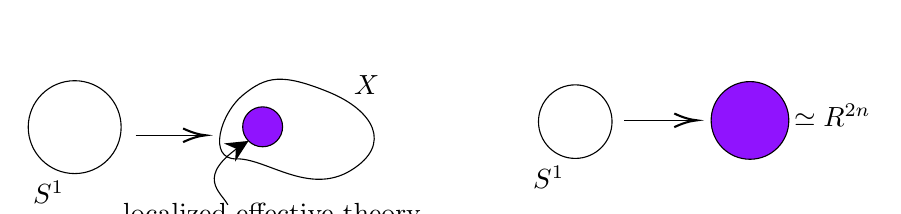
\begin{tikzpicture}[x=0.75pt,y=0.75pt,yscale=-1,xscale=1]
%Shape: Ellipse [id:dp23192014552632334] 
\draw   (34.83,63.04) .. controls (34.83,50.68) and (44.85,40.67) .. (57.21,40.67) .. controls (69.57,40.67) and (79.59,50.68) .. (79.59,63.04) .. controls (79.59,75.4) and (69.57,85.42) .. (57.21,85.42) .. controls (44.85,85.42) and (34.83,75.4) .. (34.83,63.04) -- cycle ;
%Straight Lines [id:da1794274167676957] 
\draw    (86.58,66.97) -- (118.38,66.97) ;
\draw [shift={(120.38,66.97)}, rotate = 180] [color={rgb, 255:red, 0; green, 0; blue, 0 }  ][line width=0.75]    (10.93,-3.29) .. controls (6.95,-1.4) and (3.31,-0.3) .. (0,0) .. controls (3.31,0.3) and (6.95,1.4) .. (10.93,3.29)   ;
%Shape: Polygon Curved [id:ds4925647269289568] 
\draw   (138.44,47.45) .. controls (149.5,38.5) and (157,37) .. (179.23,45.99) .. controls (201.46,54.98) and (210.5,71.5) .. (190.3,83.87) .. controls (170.1,96.23) and (149.5,78) .. (135.24,78.33) .. controls (120.97,78.66) and (127.38,56.39) .. (138.44,47.45) -- cycle ;
%Shape: Ellipse [id:dp9869721752408005] 
\draw  [fill={rgb, 255:red, 144; green, 19; blue, 254 }  ,fill opacity=1 ] (138.15,62.89) .. controls (138.15,57.58) and (142.45,53.27) .. (147.76,53.27) .. controls (153.07,53.27) and (157.38,57.58) .. (157.38,62.89) .. controls (157.38,68.2) and (153.07,72.5) .. (147.76,72.5) .. controls (142.45,72.5) and (138.15,68.2) .. (138.15,62.89) -- cycle ;
%Curve Lines [id:da32709083755427515] 
\draw    (131,100.5) .. controls (127.97,94.38) and (114.35,86.96) .. (138.6,71.18) ;
\draw [shift={(140.96,69.69)}, rotate = 148.53] [fill={rgb, 255:red, 0; green, 0; blue, 0 }  ][line width=0.08]  [draw opacity=0] (10.72,-5.15) -- (0,0) -- (10.72,5.15) -- (7.12,0) -- cycle    ;
%Shape: Ellipse [id:dp7711772783086626] 
\draw   (280.67,60.39) .. controls (280.67,50.6) and (288.6,42.67) .. (298.39,42.67) .. controls (308.18,42.67) and (316.11,50.6) .. (316.11,60.39) .. controls (316.11,70.18) and (308.18,78.11) .. (298.39,78.11) .. controls (288.6,78.11) and (280.67,70.18) .. (280.67,60.39) -- cycle ;
%Straight Lines [id:da8438423211152051] 
\draw    (322.07,59.76) -- (355.03,59.76) ;
\draw [shift={(357.03,59.76)}, rotate = 180] [color={rgb, 255:red, 0; green, 0; blue, 0 }  ][line width=0.75]    (10.93,-3.29) .. controls (6.95,-1.4) and (3.31,-0.3) .. (0,0) .. controls (3.31,0.3) and (6.95,1.4) .. (10.93,3.29)   ;
%Shape: Ellipse [id:dp2958661722082001] 
\draw  [fill={rgb, 255:red, 144; green, 19; blue, 254 }  ,fill opacity=1 ] (363.86,59.81) .. controls (363.86,49.48) and (372.24,41.1) .. (382.57,41.1) .. controls (392.91,41.1) and (401.28,49.48) .. (401.28,59.81) .. controls (401.28,70.15) and (392.91,78.52) .. (382.57,78.52) .. controls (372.24,78.52) and (363.86,70.15) .. (363.86,59.81) -- cycle ;

% Text Node
\draw (35.94,87.75) node [anchor=north west][inner sep=0.75pt]    {$S^{1}$};
% Text Node
\draw (79.29,98.35) node [anchor=north west][inner sep=0.75pt]   [align=left] {localized effective theory};
% Text Node
\draw (190.64,36.72) node [anchor=north west][inner sep=0.75pt]    {$X$};
% Text Node
\draw (276.88,80.5) node [anchor=north west][inner sep=0.75pt]    {$S^{1}$};
% Text Node
\draw (402.6,50.7) node [anchor=north west][inner sep=0.75pt]    {$\simeq \mathbb{R}^{2n}$};
\end{tikzpicture}
\end{figure}

Geometrically, a loop space is mapped to a localized neighborhood of a point in $X$ (specified by the constant map), where a localized effective theory exists.
Locally, by the choice of Darboux coordinates, $X$ can be thought of as a standard phase space, $\bR^{2n}$. 
The loop spaces are then glued together on $X$ as a family of effective field theory. This can be done rigorously within the framework of effective BV quantization:
\begin{itemize}
    \item effective action $\leadsto \gamma$,
    \item QME $\leadsto$ Fedosov equation,
    \item BV integral $\leadsto$ trace map,
    \item partition function $\leadsto$ algebraic index.
\end{itemize}
In the next section, we will present a physics ``derivation'' of the index theorem.

\section{Topological Quantum Mechanics-I}
\label{sec:tqm1}
In the \nameref{sec:dqai}, we have defined \emph{deformation quantization} from the Poisson algebra $\lb C^\infty(x), \lcb-,-\rcb_{\omega^{-1}}\rb$ to an associative algebra $\lb C^\infty(X)[[\hbar]],\star \rb$ with the canonical \emph{trace map} $\Tr: C^\infty(X)[[\hbar]] \to \bR(( \hbar))$.
In this section, we are going to prove the algebraic index theorem:
\bea \Tr(1)=\int_X e^{\omega_\hbar/\hbar} \widehat{A}(X)\eea
using the effective renormalization method in a topological quantum mechanical (TQM) model.
We follow the presentations in \cite{Gui:2019ldd,Grady:2015ica}.

\subsection{Local model}
Let's consider the standard phase space $(V,\omega)$, where $V\simeq \bR^{2n}$ with coordinates $(x^1,\cdots,x^n,x^{n+1},\cdots, x^{2n})=(q^1, \cdots, q^n, p_1,\cdots,p_n)$ and $\omega=\sum_{i=1}^n dp_i\wedge dq^i$. Let $S^1_{dR}$ be the (local ring) space with underlying topology of a circle, $S^1$, and a structure sheaf $\sO(S^1_{dR})=\Omega^\blt_{S^1}$, which is a dg (differential graded) ring of differential forms, with the de Rham differential operator $d$. 

Consider the \emph{local model}, a space of maps
\bea \varphi: S^1_{dR}\to V\simeq \bR^{2n},\eea
such that $\varphi$ can be identified with an element in $\on{Map}(S^1_{dR},V)=\Omega^\blt_{S^1}\otimes V$. Explicitly, let $\theta$ be the coordinates on $S^1$ (with the identification $\theta\sim \theta+1$). The space of maps can then be written as 
\bea \lcb\varphi \rcb= \lcb \bP_i(\theta),\bQ^i(\theta)\rcb_{i=1,\cdots,n}, \quad \bP_i,\bQ^i\in \Omega^\blt_{S^1}.\eea
Writing in form component,
\bea \bP_i(\theta)=p_i(\theta)+\eta_i(\theta)d\theta, \quad \bQ^i(\theta)=q^i(\theta)+\xi^i(\theta)d\theta.\eea
So the space of fields is 
\bea \cE= \Omega^\blt_{S^1}\otimes V\eea
and $\varphi$ is a field in $\cE$.
Then $\lb \Omega^\blt_{S^1}\otimes V, d, \int_{S^1} \lan -,-\ran_\omega\rb$ is an $\infty$-dimensional $(-1)$-dg symplectic space. The action is the free one:
\bea S\lsb \varphi\rsb &\coloneqq \int_{S^1} \lan \varphi, d\varphi\ran_\omega\\
&= \sum_i \int_{S^1} \bP_i d\bQ^i= \sum_i \int_{S^1} p_i(\theta) dq^i(\theta). \eea

\begin{rmk}
This is the first-order formalism of TQM. This is also the 1d CS theory via the \emph{Alexandrov, Kontsevich, Schwarz, Zaboronsky (AKSZ) construction}. 
\end{rmk}

\begin{rmk}
The space of local (classical) observables on $U$ is
\bea \sO(\Omega^\blt_{U}\otimes V)\simeq \sO(V),\eea
since $U$ is contractible, i.e. $\lb \Omega^\blt_{U}, d\rb\simeq \bR$. The space of global observables on $S^1$ is
\bea \sO(\Omega^\blt_{U}\otimes V) &\simeq \sO(H^\blt(S^1)\otimes V)=\sO\lb V\oplus V dt\rb\\
&=\Omega^{-\blt}_V.\eea
The map from local observables to global observables is given by the \emph{Hochschild-Kostant-Rosenberg (HKR) theorem}. As we will see, TQM gives an explicit deformed HKR when $\sO(V)$ is deformed into the Weyl algebra $\cW(V)$.
\end{rmk}

\subsection{Propagator}
Let us choose the standard flat metric on $S^1$. Let $d^\ast$ be the adjoint of $d$. The Laplacian is 
\bea \lsb d,d^\ast\rsb=-\lb \frac{d}{d\theta}\rb^2.\eea
Let 
\bea\Pi=\omega^{-1}=\sum_i \frac{\p}{\p p_i} \wedge \frac{\p}{\p q^i}= \hf \sum_i \lb \frac{\p}{\p p_i} \otimes \frac{\p}{\p q^i}- \frac{\p}{\p q^i} \otimes\frac{\p}{\p p_i}\rb \ \in \asym^2 V\eea
be the Poisson bivector (or Poisson kernel).
Let 
\bea h_t\lb \theta_1, \theta_2\rb= \frac{1}{\sqrt{4\pi t}} \sum _{n\in \bZ} e^{-\frac{\lb \theta_1-\theta_2+n\rb^2}{4t}} \eea
be the standard heat kernel on $S^1$. Then the regularized propagator is 
\bea P^L_\varepsilon =\int^L_\varepsilon \p_{\theta_1} h_t\lb \theta_1, \theta_2\rb dt \otimes \Pi \ \in \cE\otimes \cE,\eea
where $\int^L_\varepsilon \p_{\theta_1} h_t\lb \theta_1, \theta_2\rb dt  \in C^\infty(S^1 \times S^1)$ and $\Pi\in V\otimes V$. Let us denote 
\bea P^{S^1} \lb \theta_1, \theta_2\rb= \int^\infty_0 \p_{\theta_1} h_t\lb \theta_1, \theta_2\rb dt.\eea
Then the full propagator is given by 
\bea P^\infty_0= P^{S^1} \otimes \Pi.\eea

\begin{prop}
$P^{S^1} \lb \theta_1, \theta_2\rb$ is the following periodic function of $\theta_1-\theta_2 \in \bR/\bZ$ where 
\bea P^{S^1} \lb \theta_1, \theta_2\rb= \theta_1-\theta_2-\hf \quad \text{if } 0<\theta_1-\theta_2 <1.\eea
\bea \begin{tikzpicture}
    \draw [->] (-3, 0) -- (3, 0) node [right] {$\theta_1-\theta_2$};
    \draw [->] (0, -1.5) -- (0, 1.5) node [above] {$P^{S^1}$};

    \node [anchor = north east] at (-2, 0) {$-2$};
    \node [anchor = north east] at (-1, 0) {$-1$};
    \node [anchor = north east] at (0, 0) {$0$};
    \node [anchor = north east] at (1, 0) {$1$};
    \node [anchor = north east] at (2, 0) {$2$};
    
    \foreach \x in {-2, -1, 0, 1} {
      \draw [teal] (\x, -0.5) -- (\x + 1, 0.5);
    }
    \node [anchor = south east] at (0, 0.5) {$\frac{1}{2}$};
    \node [anchor = north east] at (0, -0.5) {$-\frac{1}{2}$};
    
    \node [fill, circle, inner sep = 0, minimum size = 3] at (0, 0.5) {};
    \node [fill, circle, inner sep = 0, minimum size = 3] at (0, -0.5) {};
    \node [fill, circle, inner sep = 0, minimum size = 3] at (-2, 0) {};
    \node [fill, circle, inner sep = 0, minimum size = 3] at (-1, 0) {};
    \node [fill, circle, inner sep = 0, minimum size = 3] at (1, 0) {};
    \node [fill, circle, inner sep = 0, minimum size = 3] at (2, 0) {};
\end{tikzpicture}\eea
$P^{S^1}$ is NOT a smooth function on $S^1 \times S^1$ (as expected), but it is \emph{bounded}.
\end{prop}

\subsection{Correlation map}
Let us denote the \textbf{formal Weyl algebra}
\bea \boxed{\cW_{2n}= \lb \bR [[ p_i,q^i]] ((\hbar)), \star\rb}\ ,\eea
and the \textbf{formal Weyl subalgebra}
\bea \boxed{\cW_{2n}^+ = \lb \bR [[ p_i,q^i]] [[\hbar]], \star\rb}\ ,\eea
where $\star$ is the Moyal-Weyl product. We can identify the formal Weyl subalgebra as (formal) functions on $V$ (via deformation quantization):
\bea \cW_{2n}^+ \simeq \lb\widehat{\sO}(V)[[ \hbar]], \star\rb. \eea
Given $f_0,f_1,\cdots, f_m \in \cW_{2n}$, define
$\cO_{f_0,f_1,\cdots, f_m} \in \sO(\cE)((\hbar))$
by
\bea \cO_{f_0,f_1,\cdots, f_m}\lsb \varphi\rsb\coloneqq \int_{0<\theta_1<\theta_2<\cdots<\theta_m<1} d\theta_1 d\theta_2 \cdots d\theta_m f^{(0)}_{0}\lb \varphi(\theta_0)\rb f^{(1)}_{1}\lb \varphi(\theta_1)\rb \cdots f^{(1)}_{m}\lb \varphi(\theta_m)\rb, \quad \varphi\in \Omega^\blt_{S^1}\otimes V. \eea
Here $f(\varphi(\theta))=f(\bP_i(\theta),\bQ^i(\theta))\in \Omega^\blt_{S^1}$ 
and we decompose it as 
$f(\varphi(\theta))=f^{(0)}(\varphi(\theta))+f^{(1)}(\varphi(\theta))d\theta$.
\begin{figure}[!htpb]\centering 
\tikzset{every picture/.style={line width=0.75pt}}         
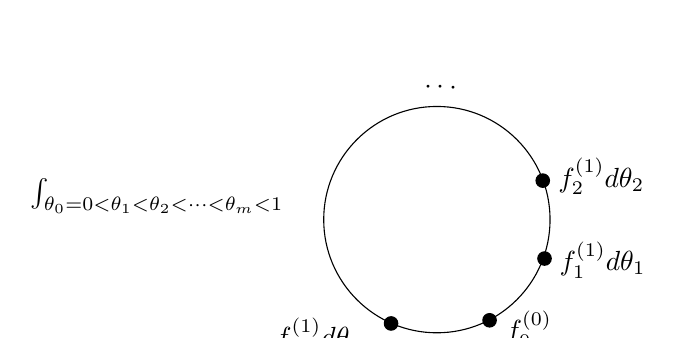
\begin{tikzpicture}[x=0.75pt,y=0.75pt,yscale=-1,xscale=1]


%Shape: Ellipse [id:dp9279145239574498] 
\draw   (392.86,103.45) .. controls (392.86,73.34) and (417.27,48.93) .. (447.39,48.93) .. controls (477.5,48.93) and (501.91,73.34) .. (501.91,103.45) .. controls (501.91,133.57) and (477.5,157.98) .. (447.39,157.98) .. controls (417.27,157.98) and (392.86,133.57) .. (392.86,103.45) -- cycle ;
%Shape: Ellipse [id:dp3458563771027001] 
\draw  [fill={rgb, 255:red, 0; green, 0; blue, 0 }  ,fill opacity=1 ] (496,122.2) .. controls (496,120.41) and (497.45,118.96) .. (499.25,118.96) .. controls (501.04,118.96) and (502.49,120.41) .. (502.49,122.2) .. controls (502.49,124) and (501.04,125.45) .. (499.25,125.45) .. controls (497.45,125.45) and (496,124) .. (496,122.2) -- cycle ;
%Shape: Ellipse [id:dp14246565917209564] 
\draw  [fill={rgb, 255:red, 0; green, 0; blue, 0 }  ,fill opacity=1 ] (469.52,151.96) .. controls (469.52,150.16) and (470.98,148.71) .. (472.77,148.71) .. controls (474.57,148.71) and (476.02,150.16) .. (476.02,151.96) .. controls (476.02,153.75) and (474.57,155.21) .. (472.77,155.21) .. controls (470.98,155.21) and (469.52,153.75) .. (469.52,151.96) -- cycle ;
%Shape: Ellipse [id:dp47308063782341825] 
\draw  [fill={rgb, 255:red, 0; green, 0; blue, 0 }  ,fill opacity=1 ] (495.14,84.66) .. controls (495.14,82.87) and (496.6,81.41) .. (498.39,81.41) .. controls (500.18,81.41) and (501.64,82.87) .. (501.64,84.66) .. controls (501.64,86.45) and (500.18,87.91) .. (498.39,87.91) .. controls (496.6,87.91) and (495.14,86.45) .. (495.14,84.66) -- cycle ;
%Shape: Ellipse [id:dp014766617978020369] 
\draw  [fill={rgb, 255:red, 0; green, 0; blue, 0 }  ,fill opacity=1 ] (422.06,153.48) .. controls (422.06,151.68) and (423.51,150.23) .. (425.31,150.23) .. controls (427.1,150.23) and (428.55,151.68) .. (428.55,153.48) .. controls (428.55,155.27) and (427.1,156.73) .. (425.31,156.73) .. controls (423.51,156.73) and (422.06,155.27) .. (422.06,153.48) -- cycle ;

% Text Node
\draw (479.27,146.11) node [anchor=north west][inner sep=0.75pt]    {$f_{0}^{( 0)}$};
% Text Node
\draw (368.21,149.41) node [anchor=north west][inner sep=0.75pt]    {$f_{m}^{( 1)} d\theta _{m}$};
% Text Node
\draw (449.27,40) node  [rotate=-1.35]  {$\cdots $};
% Text Node
\draw (505.25,112.86) node [anchor=north west][inner sep=0.75pt]    {$f_{1}^{( 1)} d\theta _{1}$};
% Text Node
\draw (504.64,72.56) node [anchor=north west][inner sep=0.75pt]    {$f_{2}^{( 1)} d\theta _{2}$};
% Text Node
\draw (250.5,82.4) node [anchor=north west][inner sep=0.75pt]    {$\int _{\theta _{0} =0< \theta _{1} < \theta _{2} < \cdots < \theta _{m} < 1}$};
\end{tikzpicture}
\end{figure}

\begin{rmk}
$f^{(1)}(\varphi)$ is the \textbf{topological descent} of $f^{(0)}(\varphi)$ (in the sense of Witten \cite{witten1987elliptic,Witten:1987cg}).
\end{rmk}

Now let's apply the HRG flow, $\exp{(\hbar P^\infty_0)}\lb \cO_{f_0,f_1,\cdots, f_m}\rb$. Since $P^\infty_0$ is bounded, it is convergent and well-defined! This is a \emph{UV finite property}.

As we have discussed, at $L=\infty$, we can view it as defining a function on zero modes on 
\bea\bH &=H^\blt\lb \Omega^\blt_{S^1} \otimes V, d\rb= H^\blt(S^1)\otimes V\\
&= V\oplus V d\theta.\eea
We have $\widehat{\sO}(\bH)=\widehat{\Omega}^{-\blt}_{2n}$ forms on $V$.

\begin{defn}
We define the following correlation map:
\bea \lan \cdots\ran_{free}: \cW_{2n} \otimes \cdots \otimes \cW_{2n} \to \widehat{\Omega}^{-\blt}_{2n}((\hbar))\eea
by $\lan f_0\otimes f_1\otimes \cdots\otimes f_m\ran_{free} \coloneqq \left. \exp{(\hbar P^\infty_0)}\lb \cO_{f_0,f_1,\cdots, f_m}\rb \right|_{\bH}$.
In the path integral perspective, this is 
\bea \lan f_0\otimes f_1\otimes \cdots\otimes f_m\ran_{free}(\alpha)
=\int_{\Im d^\ast \subset \cE} \lsb D\varphi\rsb e^{-S[\varphi+\alpha]/\hbar} \cO_{f_0,f_1,\cdots,f_m}[\varphi+\alpha], \quad \alpha\in \bH= H^\blt(S^1)\otimes V.\eea
$\alpha$ is essentially the background field. It can also be represented as a Feynman diagram as follows.
\begin{figure}[!htpb]\centering 
\tikzset{every picture/.style={line width=0.75pt}}         
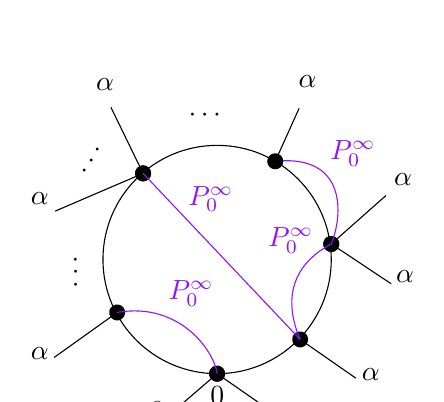
\begin{tikzpicture}[x=0.75pt,y=0.75pt,yscale=-1,xscale=1]


%Shape: Circle [id:dp32266046359972234] 
\draw   (370.33,193.5) .. controls (370.33,163.12) and (394.96,138.5) .. (425.33,138.5) .. controls (455.71,138.5) and (480.33,163.12) .. (480.33,193.5) .. controls (480.33,223.88) and (455.71,248.5) .. (425.33,248.5) .. controls (394.96,248.5) and (370.33,223.88) .. (370.33,193.5) -- cycle ;
%Straight Lines [id:da8359020571133517] 
\draw    (374.17,120.17) -- (389.67,152) ;
\draw [shift={(389.67,152)}, rotate = 64.04] [color={rgb, 255:red, 0; green, 0; blue, 0 }  ][fill={rgb, 255:red, 0; green, 0; blue, 0 }  ][line width=0.75]      (0, 0) circle [x radius= 3.35, y radius= 3.35]   ;
%Straight Lines [id:da7986088148712582] 
\draw    (347.33,170.17) -- (389.67,152) ;
\draw [shift={(389.67,152)}, rotate = 336.77] [color={rgb, 255:red, 0; green, 0; blue, 0 }  ][fill={rgb, 255:red, 0; green, 0; blue, 0 }  ][line width=0.75]      (0, 0) circle [x radius= 3.35, y radius= 3.35]   ;
%Straight Lines [id:da8708432649210969] 
\draw    (346.83,240.67) -- (377.17,219) ;
\draw [shift={(377.17,219)}, rotate = 324.46] [color={rgb, 255:red, 0; green, 0; blue, 0 }  ][fill={rgb, 255:red, 0; green, 0; blue, 0 }  ][line width=0.75]      (0, 0) circle [x radius= 3.35, y radius= 3.35]   ;
%Straight Lines [id:da15766790265263397] 
\draw    (403.67,267.17) -- (425.33,248.5) ;
\draw [shift={(425.33,248.5)}, rotate = 319.25] [color={rgb, 255:red, 0; green, 0; blue, 0 }  ][fill={rgb, 255:red, 0; green, 0; blue, 0 }  ][line width=0.75]      (0, 0) circle [x radius= 3.35, y radius= 3.35]   ;
%Straight Lines [id:da17957602222249913] 
\draw    (452.17,267.17) -- (425.33,248.5) ;
\draw [shift={(425.33,248.5)}, rotate = 214.82] [color={rgb, 255:red, 0; green, 0; blue, 0 }  ][fill={rgb, 255:red, 0; green, 0; blue, 0 }  ][line width=0.75]      (0, 0) circle [x radius= 3.35, y radius= 3.35]   ;
%Straight Lines [id:da3682811688121579] 
\draw    (492.17,250.67) -- (465.33,232) ;
\draw [shift={(465.33,232)}, rotate = 214.82] [color={rgb, 255:red, 0; green, 0; blue, 0 }  ][fill={rgb, 255:red, 0; green, 0; blue, 0 }  ][line width=0.75]      (0, 0) circle [x radius= 3.35, y radius= 3.35]   ;
%Straight Lines [id:da6871435476196512] 
\draw    (509.17,205.17) -- (480.33,186) ;
\draw [shift={(480.33,186)}, rotate = 213.61] [color={rgb, 255:red, 0; green, 0; blue, 0 }  ][fill={rgb, 255:red, 0; green, 0; blue, 0 }  ][line width=0.75]      (0, 0) circle [x radius= 3.35, y radius= 3.35]   ;
%Straight Lines [id:da2213504058401865] 
\draw    (506.67,162.67) -- (480.33,186) ;
\draw [shift={(480.33,186)}, rotate = 138.46] [color={rgb, 255:red, 0; green, 0; blue, 0 }  ][fill={rgb, 255:red, 0; green, 0; blue, 0 }  ][line width=0.75]      (0, 0) circle [x radius= 3.35, y radius= 3.35]   ;
%Curve Lines [id:da8638832915566401] 
\draw [color={rgb, 255:red, 144; green, 19; blue, 254 }  ,draw opacity=1 ]   (377.17,219) .. controls (407.67,213.67) and (424.17,238.17) .. (425.33,248.5) ;
%Curve Lines [id:da033505788594483166] 
\draw [color={rgb, 255:red, 144; green, 19; blue, 254 }  ,draw opacity=1 ]   (480.33,186) .. controls (461.5,196) and (457,212.5) .. (465.33,232) ;
%Curve Lines [id:da045835240771453956] 
\draw [color={rgb, 255:red, 144; green, 19; blue, 254 }  ,draw opacity=1 ]   (453.33,146.17) .. controls (488.33,142.67) and (485.83,172.67) .. (480.33,186) ;
%Straight Lines [id:da3518391071014495] 
\draw    (464.83,120.67) -- (453.33,146.17) ;
\draw [shift={(453.33,146.17)}, rotate = 114.27] [color={rgb, 255:red, 0; green, 0; blue, 0 }  ][fill={rgb, 255:red, 0; green, 0; blue, 0 }  ][line width=0.75]      (0, 0) circle [x radius= 3.35, y radius= 3.35]   ;
%Straight Lines [id:da5327889741402634] 
\draw [color={rgb, 255:red, 144; green, 19; blue, 254 }  ,draw opacity=1 ]   (389.67,152) -- (465.33,232) ;

% Text Node
\draw (400.67,202.4) node [anchor=north west][inner sep=0.75pt]  [color={rgb, 255:red, 144; green, 19; blue, 254 }  ,opacity=1 ]  {$P_{0}^{\infty }$};
% Text Node
\draw (410.17,156.9) node [anchor=north west][inner sep=0.75pt]  [color={rgb, 255:red, 144; green, 19; blue, 254 }  ,opacity=1 ]  {$P_{0}^{\infty }$};
% Text Node
\draw (448.67,176.9) node [anchor=north west][inner sep=0.75pt]  [color={rgb, 255:red, 144; green, 19; blue, 254 }  ,opacity=1 ]  {$P_{0}^{\infty }$};
% Text Node
\draw (478.67,134.9) node [anchor=north west][inner sep=0.75pt]  [color={rgb, 255:red, 144; green, 19; blue, 254 }  ,opacity=1 ]  {$P_{0}^{\infty }$};
% Text Node
\draw (334.33,234.9) node [anchor=north west][inner sep=0.75pt]    {$\alpha $};
% Text Node
\draw (334.33,159.9) node [anchor=north west][inner sep=0.75pt]    {$\alpha $};
% Text Node
\draw (365.83,104.9) node [anchor=north west][inner sep=0.75pt]    {$\alpha $};
% Text Node
\draw (391.33,260.9) node [anchor=north west][inner sep=0.75pt]    {$\alpha $};
% Text Node
\draw (451.33,261.9) node [anchor=north west][inner sep=0.75pt]    {$\alpha $};
% Text Node
\draw (493.83,244.9) node [anchor=north west][inner sep=0.75pt]    {$\alpha $};
% Text Node
\draw (510.33,197.4) node [anchor=north west][inner sep=0.75pt]    {$\alpha $};
% Text Node
\draw (509.33,150.9) node [anchor=north west][inner sep=0.75pt]    {$\alpha $};
% Text Node
\draw (463.33,103.4) node [anchor=north west][inner sep=0.75pt]    {$\alpha $};
% Text Node
\draw (353.34,208.55) node [anchor=north west][inner sep=0.75pt]  [rotate=-269.59]  {$\cdots $};
% Text Node
\draw (410.4,119.77) node [anchor=north west][inner sep=0.75pt]  [rotate=-0.52]  {$\cdots $};
% Text Node
\draw (420.83,253.4) node [anchor=north west][inner sep=0.75pt]    {$0$};
% Text Node
\draw (356.67,151.21) node [anchor=north west][inner sep=0.75pt]  [rotate=-302.24]  {$\cdots $};
\end{tikzpicture}
\end{figure}
\end{defn}

\paragraph{(Cyclic) Hochschild complex reviewed.}
Let $A$ be a unital associative algebra and $\ols{A} \coloneqq A/(\bC\cdot 1)$. Let $C_{-p}(A)\coloneqq A\otimes \ols{A}^{\otimes p}$ be the cyclic $p$-chains. It carries a natural \textbf{Hochschild differential}
\bea b: C_{-p}(A) \to C_{-p+1}(A), \quad p\geq 1\eea
by $b(a_0\otimes \cdots\otimes a_p)=(-1)^{p} a_p a_0\otimes \cdots\otimes a_{p-1}+\sum_{i=0}^{p-1} (-1)^i a_0\otimes \cdots\otimes a_{i}a_{i+1} \otimes\cdots\otimes a_p$. 
\bea 
\tikzset{every picture/.style={line width=0.75pt}}
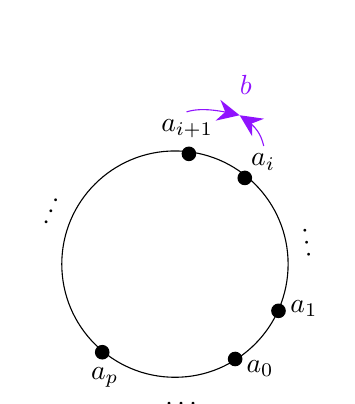
\begin{tikzpicture}[x=0.75pt,y=0.75pt,yscale=-1,xscale=1]

%Shape: Ellipse [id:dp7120147372059156] 
\draw   (44.9,196.45) .. controls (44.9,166.34) and (69.31,141.93) .. (99.43,141.93) .. controls (129.54,141.93) and (153.95,166.34) .. (153.95,196.45) .. controls (153.95,226.57) and (129.54,250.98) .. (99.43,250.98) .. controls (69.31,250.98) and (44.9,226.57) .. (44.9,196.45) -- cycle ;
%Shape: Ellipse [id:dp5538374474188836] 
\draw  [fill={rgb, 255:red, 0; green, 0; blue, 0 }  ,fill opacity=1 ] (102.91,143.32) .. controls (102.91,141.52) and (104.36,140.07) .. (106.16,140.07) .. controls (107.95,140.07) and (109.4,141.52) .. (109.4,143.32) .. controls (109.4,145.11) and (107.95,146.57) .. (106.16,146.57) .. controls (104.36,146.57) and (102.91,145.11) .. (102.91,143.32) -- cycle ;
%Shape: Ellipse [id:dp10713447671859067] 
\draw  [fill={rgb, 255:red, 0; green, 0; blue, 0 }  ,fill opacity=1 ] (129.82,154.92) .. controls (129.82,153.13) and (131.28,151.67) .. (133.07,151.67) .. controls (134.86,151.67) and (136.32,153.13) .. (136.32,154.92) .. controls (136.32,156.71) and (134.86,158.17) .. (133.07,158.17) .. controls (131.28,158.17) and (129.82,156.71) .. (129.82,154.92) -- cycle ;
%Shape: Ellipse [id:dp9918190740335271] 
\draw  [fill={rgb, 255:red, 0; green, 0; blue, 0 }  ,fill opacity=1 ] (146.06,218.96) .. controls (146.06,217.16) and (147.52,215.71) .. (149.31,215.71) .. controls (151.11,215.71) and (152.56,217.16) .. (152.56,218.96) .. controls (152.56,220.75) and (151.11,222.21) .. (149.31,222.21) .. controls (147.52,222.21) and (146.06,220.75) .. (146.06,218.96) -- cycle ;
%Shape: Ellipse [id:dp6415609432002995] 
\draw  [fill={rgb, 255:red, 0; green, 0; blue, 0 }  ,fill opacity=1 ] (125.18,242.16) .. controls (125.18,240.37) and (126.64,238.91) .. (128.43,238.91) .. controls (130.22,238.91) and (131.68,240.37) .. (131.68,242.16) .. controls (131.68,243.95) and (130.22,245.41) .. (128.43,245.41) .. controls (126.64,245.41) and (125.18,243.95) .. (125.18,242.16) -- cycle ;
%Shape: Ellipse [id:dp8927580999760203] 
\draw  [fill={rgb, 255:red, 0; green, 0; blue, 0 }  ,fill opacity=1 ] (61.14,238.91) .. controls (61.14,237.12) and (62.6,235.66) .. (64.39,235.66) .. controls (66.19,235.66) and (67.64,237.12) .. (67.64,238.91) .. controls (67.64,240.71) and (66.19,242.16) .. (64.39,242.16) .. controls (62.6,242.16) and (61.14,240.71) .. (61.14,238.91) -- cycle ;
%Curve Lines [id:da00012053268975198428] 
\draw [color={rgb, 255:red, 144; green, 19; blue, 254 }  ,draw opacity=1 ]   (142.2,139.53) .. controls (140.79,133.55) and (138.45,130.35) .. (133.01,126.4) ;
\draw [shift={(130.6,124.73)}, rotate = 33.69] [fill={rgb, 255:red, 144; green, 19; blue, 254 }  ,fill opacity=1 ][line width=0.08]  [draw opacity=0] (10.72,-5.15) -- (0,0) -- (10.72,5.15) -- (7.12,0) -- cycle    ;
%Curve Lines [id:da8367737837485085] 
\draw [color={rgb, 255:red, 144; green, 19; blue, 254 }  ,draw opacity=1 ]   (127.62,124.04) .. controls (121.65,122.66) and (112.06,120.78) .. (105,123.13) ;
\draw [shift={(130.6,124.73)}, rotate = 192.99] [fill={rgb, 255:red, 144; green, 19; blue, 254 }  ,fill opacity=1 ][line width=0.08]  [draw opacity=0] (10.72,-5.15) -- (0,0) -- (10.72,5.15) -- (7.12,0) -- cycle    ;

% Text Node
\draw (91.58,125.59) node [anchor=north west][inner sep=0.75pt]    {$a_{i+1}$};
% Text Node
\draw (134.89,142.11) node [anchor=north west][inner sep=0.75pt]    {$a_{i}$};
% Text Node
\draw (153.8,212.68) node [anchor=north west][inner sep=0.75pt]    {$a_{1}$};
% Text Node
\draw (132.67,241.45) node [anchor=north west][inner sep=0.75pt]    {$a_{0}$};
% Text Node
\draw (57.75,244.91) node [anchor=north west][inner sep=0.75pt]    {$a_{p}$};
% Text Node
\draw (129.39,104.14) node [anchor=north west][inner sep=0.75pt]  [color={rgb, 255:red, 144; green, 19; blue, 254 }  ,opacity=1 ]  {$b$};
% Text Node
\draw (40,171.15) node  [rotate=-292.57]  {$\cdots $};
% Text Node
\draw (102.65,264) node  [rotate=-1.35]  {$\cdots $};
% Text Node
\draw (163.33,186) node  [rotate=-261.64]  {$\cdots $};
\end{tikzpicture}
\eea
Then the associativity implies 
$b\circ b=0$. Thus,
$(C_{-\blt}(A), b)$ defines the \textbf{Hochschild chain complex}.

We can also define the \textbf{Connes operator}:
\bea B: C_{-p}(A) \to C_{-p-1}(A)\eea
by $B(a_0\otimes \cdots\otimes a_p)=1\otimes a_0 \otimes\cdots\otimes a_p+\sum_{i=1}^p (-1)^{pi} 1\otimes a_i \otimes\cdots\otimes a_p\otimes a_0 \otimes\cdots\otimes a_{i-1}.$
We have the following relations:
\bea b^2=0, \quad B^2=0, \quad [b,B]=bB+Bb=0.\eea
Let $u$ be a formal variable of $\on{deg}=2$. Then $(b+uB)^2=0$.
This defines a complex
\bea CC^{per}_{-\blt}(A)=\lb C_{-\blt}(A)[u,u^{-1}], b+uB\rb,\eea
called the \textbf{periodic cyclic complex}.

\paragraph{Correlation map.}
It is not hard to see via type reason that
\bea \lan \cdots\ran_{free}: C_{-p}\lb \cW_{2n}\rb \to \widehat{\Omega}^{-p}_{2n}((\hbar)),\eea
i.e. $\lan f_0\otimes f_1\otimes \cdots\otimes f_p\ran_{free}$ is a $p$-form. Recall that $\widehat{\Omega}^{-\blt}_{2n}$ is equipped with a BV operator $\Delta=\cL_{\omega^{-1}}=\cL_\Pi$.

\begin{prop}
\bea \lan b(-)\ran_{free}= \hbar \Delta \lan \cdots\ran_{free},\\
\lan B(-)\ran_{free}= d_{2n} \lan \cdots\ran_{free}.\eea
\end{prop}
Here $d_{2n}: \widehat{\Omega}^{-\blt}_{2n} \to \widehat{\Omega}^{-(\blt+1)}_{2n}$ is the de Rham differential. In other words, the \textbf{correlation map}:
\bea  \lan \cdots\ran_{free}: C_{-\blt}(\cW_{2n}) \to \widehat{\Omega}^{-\blt}_{2n}((\hbar ))\eea
intertwines $b$ with $\hbar\Delta$ and $B$ with $d_{2n}$. We can combine the above two equations and get
\bea \lan\cdots\ran_{free}: CC^{per}_{-\blt}(\cW_{2n})\to 
\widehat{\Omega}^{-\blt}_{2n}((\hbar))[u,u^{-1}], \quad b+uB \mapsto h\Delta+ud_{2n}.\eea

\subsection{BV integral on zero modes}
We can define a \emph{BV integration} map on the BV algebra $\lb \widehat{\Omega}^{-\blt}_{2n},\Delta\rb$
which is only non-zero on top forms $\widehat{\Omega}^{-2n}_{2n}$ and sends
\bea \beta\in \widehat{\Omega}^{-2n}_{2n} \mapsto \left. \frac{\hbar^n}{n!}\iota^n_\Pi \beta \right|_{p=q=0}.\eea
This is the \textbf{Berezin integral} over the purely fermionic superLagrangian. We can extend this BV integration to an $S^1$-equivariant version by
\bea \int_{BV}: \widehat{\Omega}^{-\blt}_{2n}[u,u^{-1}] \to \bR((\hbar))[u,u^{-1}], \quad \beta\mapsto \left. \lb u^n e^{\hbar\iota_\Pi/u}\beta\rb\right|_{p=q=0}.\eea
Then it has the following property
\bea \int_{BV} \lb \hbar\Delta +ud_{2n}\rb(-)=0\eea

\begin{rmk}
For $\beta\in \widehat{\Omega}^{-\blt}_{2n}$, the equivariant limit
\bea \lim_{u\to\infty} \int_{BV} \beta= \left. \frac{\hbar^n}{n!}\iota_\Pi^n \beta\right|_{p=q=0}\eea
gives back the Berezin integral.
\end{rmk}

Combining the above maps, we define
\bea \Tr \coloneqq \int_{BV}  \circ \lan \cdots\ran_{free}: CC^{per}_{-\blt}(\cW_{2n})\to \bR((\hbar))[u,u^{-1}]\eea
which satisfies the following equation:
\bea\Tr\lb (b+uB)(-)\rb=0.\eea
Therefore $\Tr$ descends to \textbf{periodic cyclic homology}. This is essentially the \textbf{Feigin-Felder-Shoikhet formula}.

\paragraph{A graded version.}
We can generalize slightly by considering a graded vector space $V$ with a $\on{deg}=0$ symplectic pairing $\omega$. We still have the canonical quantization $\lb \widehat{\sO}(V)[[ \hbar]],\star\rb$ and similarly can define the BV algebra of forms $\lb \widehat{\Omega}^{-\blt}_{V},\Delta=\cL_{\omega^{-1}}\rb$.
The same trace map gives 
\bea \lan \cdots\ran_{free}: C_{-\blt}\lb \widehat{\sO}(V)[[\hbar]]\rb\to 
\widehat{\Omega}^{-\blt}_{V}((\hbar)), \quad b\mapsto \hbar\Delta.\eea
Given $\gamma\in \widehat{\sO}(V)[[\hbar]]$, $\on{deg}(\gamma)=1$, it defines an action functional:
\bea I_\gamma= \int_{S^1}\gamma(\varphi) \quad \forall \varphi\in \Omega^\blt(S^1)\otimes V.\eea
Let's treat $I_\gamma$ as an \textbf{interaction} and consider
\bea \underbrace{\hf \int_{S^1} \lan \varphi,d\varphi\ran}_{\text{free part}}
+\underbrace{\int_{S^1} \gamma(\varphi)}_{I_\gamma}.\eea
Then we run the HRG flow to get
\bea e^{\frac{1}{\hbar}I_\gamma[\infty]}\coloneqq \exp{(\hbar P^\infty_0)} e^{\frac{1}{\hbar}I_\gamma}\eea
which is well-defined since $P^\infty_0$ is bounded.

Let's now analyze the QME. By construction,
\bea e^{\frac{1}{\hbar}I_\gamma[\infty]}= \lan 1\otimes e^{\gamma/\hbar}\ran_{free}.\eea
Assume $\gamma\star \gamma=\hf \lsb \gamma,\gamma\rsb_\star=0$. Then 
\bea \hbar\Delta e^{\frac{1}{\hbar}I_\gamma[\infty]}= \lan b\lb 1\otimes e^{\gamma/\hbar}\rb \ran_{free}=0.\eea

\begin{prop}[Grady-Li-L]
If $\lsb \gamma,\gamma\rsb_\star=0$, then the local interaction $I_\gamma= \int_{S^1} \gamma(\varphi)$ defines a family of solutions of effective QME $I_\gamma[L]$ at scale $L>0$ by
\bea e^{\frac{1}{\hbar}I_\gamma[L]}\coloneqq \lim_{\varepsilon\to\infty} \exp{(\hbar P^L_\varepsilon)} e^{\frac{1}{\hbar}I_\gamma}.\eea
\end{prop}














































 
\section{Topological Quantum Mechanics-II}
\label{sec:tqm2}

Recall in \nameref{sec:tqm1}, we have discussed the first-order formalism of TQM such that in a local model with maps $\varphi: \Omega^\blt_{S^1} \to V\simeq \bR^{2n}$, the correlation map
\bea  \lan \cdots\ran_{free}: C_{-\blt}(\cW_{2n}) \to \widehat{\Omega}^{-\blt}_{2n}((\hbar ))\eea
intertwines $b$ with $\hbar\Delta$ and $B$ with $d_{2n}$.

In this section, we are going to glue this construction to a symplectic manifold and establish the algebraic index to universal Lie algebra
cohomology computations. The basic idea is to \emph{glue} the local model $\Sigma\to T^{Model}\subset X$. 
\textsc{Reference}: \cite{Gui:2019ldd}

\subsection{Gluing via Gelfand-Kazhdan formal geometry}
\begin{defn}
A \textbf{Harish-Chandra pair} is a pair $(\fg,K)$, where $\fg$ is a Lie algebra, $K$ is a Lie group, with 
\begin{itemize}
    \item an action of $K$ on $\fg$: $K\xrightarrow{\ \rho\ } \on{Aut}(\fg)$,
    \item a natural embedding: $\on{Lie}(K) \xhookrightarrow{\ i\ } \fg$, where $\on{Lie}(K)$ is the Lie algebra associated with $K$,
\end{itemize}
such that they are compatible:
\bea
\begin{tikzcd}
\on{Lie}(K) \ar[r, hook, "i"] \ar[dr, "d\rho"]
& \fg \ar[d,"adjoint"] \\
& \on{Der}(\fg)
\end{tikzcd}
\eea
\end{defn}

\begin{defn}
A \textbf{$(\fg,K)$-module} is a vector space $V$ with 
\begin{itemize}
    \item an action of $K$ on $V$: $K \xrightarrow{\ \varphi\ } \on{GL}(V)$,
    \item a Lie algebra morphism: $\fg\to \on{End}(V)$,
\end{itemize}
such that they are compatible:
\bea
\begin{tikzcd}
\on{Lie}(K) \ar[r, hook, "i"] \ar[dr, "d\varphi"]
& \fg \ar[d] \\
& \on{End}(V)
\end{tikzcd}
\eea
\end{defn}

\begin{defn}
A \textbf{flat $(\fg,K)$-bundle} over X is
\begin{itemize}
    \item a principal $K$-bundle $P \xrightarrow{\ \pi\ } X$,
    \item a $K$-equivariant $\fg$-valued 1-form $\gamma\in \Omega^1(P,\fg)$ on $P$,
\end{itemize}
satisfying the following conditions:
\bi[(1)]
    \item $\forall a\in \on{Lie}(K)$, let $\xi_a\in \on{Vect}(P)$ generated by $a$. Then we have the contraction $\gamma(\xi_a)=a$ such that
    \bea
    \begin{tikzcd}
        0 \ar[r] & \on{Lie}(K) \ar[r] \ar[dr, hook, "i"] & \on{Vect}(P) \ar[d, "\gamma"] \\
        & & \fg
    \end{tikzcd}
    \eea
    \item $\gamma$ satisfies the Maurer-Cartan equation
    \bea d\gamma +\hf \lsb \gamma,\gamma\rsb=0,\eea
    where $d$ is the de Rham differential on $P$, and $\lsb-,-\rsb$ is the Lie bracket in $\fg$.
\ei
\end{defn}

Given a flat $(\fg,K)$-bundle $P\to X$ and $(\fg,K)$-module $V$, let \bea\Omega^\blt(P,V)\coloneqq \Omega^\blt (P)\otimes V\eea
denote differential forms on $P$ valued in $V$.
It carries a connection
\bea \nabla^\gamma= d+\gamma :  \Omega^\blt(P,V)\to \Omega^{\blt+1}(P,V)\eea
which is \emph{flat} by the Maurer-Cartan equation.
The group $K$ acts on $\Omega^\blt(P)$ and $V$, and hence inducing a natural action on $\Omega^\blt(P,V)$.

Let 
\bea V_P\coloneqq P \times_K V\eea 
be the vector bundle on $X$ associated to the $K$-representation $V$. Let $\Omega^\blt(X;V_P)$ be differential forms
on $X$ valued in the bundle $V_P\to X$.
Similar to the usual principal bundle case, $\nabla^\gamma$ induces a flat connection on $V_P\to X$. This defines a (de Rham) chain complex $\lb \Omega^\blt(X;V_P), \nabla^\gamma\rb$, and $H^\blt(X;V_P)$ denotes the corresponding de Rham cohomology.

Next we discuss how to descend Lie algebra cohomologies to geometric objects on $X$.
\begin{defn}
Let $V$ be a $(\fg,K)$-module. Define the \textbf{$(\fg,K)$ relative Lie algebra cochain complex} 
$\lb C^\blt_{Lie}(\fg,K;V), \p_{Lie}\rb$
by
\bea C^p_{Lie}(\fg,K;V)=\on{Hom}_K \lb \asym^p\lb\fg/\on{Lie}(K)\rb,V\rb.\eea
\end{defn}
Here $\on{Hom}_K$ means $K$-equivariant linear maps. $\p_{Lie}$ is the Chevalley-Eilenberg differential if we view
$C^p_{Lie}(\fg,K;V)$ as a subspace of the Lie algebra cochain $C^p_{Lie}(\fg;V)$. Explicitly,
for $\alpha\in C^p_{Lie}(\fg,K;V)$,
\bea \lb \p_{Lie}\alpha\rb \lb a_1 \wedge \cdots \wedge a_{p+1}\rb
&=\sum_{i=1}^{p+1}(-1)^{i-1} a_i\cdot \alpha\lb a_1 \wedge \cdots \wedge \widehat{a}_i \wedge \cdots \wedge a_{p+1}\rb\\
&\quad +\sum_{i<j} (-1)^{i+j} \alpha\lb \lsb a_i,a_j\rsb \wedge \cdots \wedge \widehat{a}_i \wedge \cdots \wedge \widehat{a}_j \wedge \cdots \wedge a_{p+1}\rb.\eea
The corresponding cohomology is $H^\blt_{Lie}(\fg,K;V)$. 

Given a $(\fg,K)$-module $V$ and flat $(\fg,K)$-bundle $P\to X$ with the flat connection $\gamma\in\Omega^1(P,\fg)$. 
We can define the \textbf{descent map} from the $(\fg, K)$ relative Lie algebra cochain complex to
$V$-valued de Rham complex on $P$ by
\bea \on{desc}: \lb C^\blt_{Lie}(\fg,K;V),\p_{Lie}\rb\to \lb \Omega^\blt(X;V_P),\nabla^\gamma\rb, \quad \alpha\mapsto \alpha(\gamma,\cdots,\gamma)\eea
inducing the cohomology descent map
\bea \on{desc}: H^\blt_{Lie}(\fg,K;V)\to H^\blt (X;V_P).\eea

\subsection{Fedosov connection revisited}
Recall the (formal) Weyl algebras
\bea \cW_{2n}=\bR[[p_i,q^i]] ((\hbar)), \quad 
\cW_{2n}^+=\bR[[p_i,q^i]] [[\hbar]]\eea
with the induced Lie algebra structure such that the Lie bracket is defined by
\bea \lsb f,g\rsb\coloneqq \frac{1}{\hbar} \lsb f,g\rsb_\star=\frac{1}{\hbar}\lb f\star g- g\star f\rb.\eea

Let $\gsp_{2n}$ be the symplectic group of linear transformations preserving the Poisson bivector $\Pi$. It acts on Weyl algebras by inner automorphisms. We can identify the Lie algebra $\sp_{2n}$ of $\gsp_{2n}$ with the quadratic polynomial in $\bR[p_i,q^i]$, and $\sp_{2n}$ is a Lie subalgebra of $\cW_{2n}^+$.
The action $\gsp_{2n}\curvearrowright \bR^{2n}$ induces $\gsp_{2n}\curvearrowright \cW_{2n}^+$. Hence, $\lb \cW_{2n}^+,\gsp_{2n}\rb$ and $\lb \cW_{2n},\gsp_{2n}\rb$ are Harish-Chandra pairs.

Let $(X,\omega)$ be a symplectic manifold, and $F_{\gsp}(X)$ be the symplectic frame bundle. We have the Weyl bundles
\bea \cW^+_X=F_{\gsp}(X)\times_{\gsp_{2n}} \cW_{2n}^+, \quad 
\cW_X=F_{\gsp}(X) \times_{\gsp_{2n}} \cW_{2n}.\eea
Consider the Harish-Chandra pair
\bea (\ols{\fg},K)=(\fg/Z(\fg),\gsp_{2n}),\eea
where $\fg=\cW_{2n}^+$, and $Z(\fg)=\bR[[\hbar]]$ is the center of $\fg$, $Z(\fg)\cap \sp_{2n}=0$.
Fedosov constructed a flat $(\ols{\fg},K)$-bundle $F_{\gsp}(X)\to X$
and $H^0(X; \cW_X^+)$ gives a \emph{deformation quantization}. 
Choose the trivial $(\ols{\fg},K)$-module $\bR((\hbar))$. Then 
\bea \on{desc}: C^\blt_{Lie} \lb \ols{\cW^+_{2n}},\sp_{2n}; \bR((\hbar))\rb \to \Omega^\blt_X((\hbar)).\eea 
This is the \textbf{Gelfand-Fuks map}.
Here $C^\blt_{Lie} \lb \ols{\cW^+_{2n}},\sp_{2n}; \bR((\hbar))\rb \simeq C^\blt_{Lie}\lb \cW^+_{2n},\sp_{2n}\oplus Z(\cW^+_{2n}); \bR((\hbar))\rb$.

\subsection{Characteristic classes}
Let us review the Chern-Weil construction of \emph{characteristic classes} in Lie algebra cohomology.
They will descent to the usual characteristic forms via the Gelfand-Fuks map.

Let $\fg$ be a Lie algebra, and $\fh\subset \fg$ be its Lie subalgebra. Let the projection map
\bea \on{pr}: \fg\to\fh\eea
be the $\fh$-equivariant splitting of the embedding $\fh\subset \fg$. In general $\on{pr}$ is not a Lie algebra homomorphism from $\fg$ to $\fh$. The \emph{failure} of $\on{pr}$ being a Lie algebra homomorphism gives $R\in \on{Hom}\lb \asym^2\fg, \fh\rb$ by
\bea R(\alpha,\beta)=\lsb \on{pr}(\alpha),\on{pr}(\beta)\rsb_\fh-\on{pr}\lsb \alpha,\beta\rsb_\fg, \quad \alpha,\beta\in\fg.\eea
The $\fh$-equivariance of $\on{pr}$ implies that $R\in\on{Hom}_\fh\lb \asym^2(\fg/\fh),\fh\rb$. $R$ is called the \textbf{curvature form}.
Let $\sym^m(\fh^\vee)^\fh$ be $\fh$-invariant polynomials on $\fh$ of homogeneous degree $\on{deg}=m$. Given $P\in \sym^m(\fh^\vee)^\fh$, 
we can
associate a cochain $P(R)\in C^{2m}_{Lie}(\fg, \fh; \bR)$ by the composition
\bea P(R): \asym^{2m}\fg \xrightarrow{\asym^m R} \sym^m(\fh) \xrightarrow{P}\bR.\eea
It can be checked that $\p_{Lie} P(R)=0$, defining a cohomology class $[P(R)]$ in $H^{2m}(\fg,\fh;\bR)$ which does
not depend on the choice of $\on{pr}$. Therefore we have the analogue of Chern-Weil characteristic map
\bea \chi:\sym^\blt(\fh^\vee)^\fh \to H^\blt(\fg,\fh;\bR), \quad P\mapsto \chi(P) \coloneqq \lsb P(R)\rsb.\eea

Now we apply the above construction to the case where
\bea \fg= \cW^+_{2n}, \quad \fh=\sp_{2n}\oplus Z(\fg).\eea
Any element $f$ in $\fg= \cW^+_{2n}$ can be uniquely written as a polynomial
$f=f(y^i,\hbar)$, with coordinates $(y^1,\cdots,y^n,y^{n+1},\cdots, y^{2n})=(p_1,\cdots,p_n, q^1, \cdots, q^n)$. 
Define the $\fh$-equivariant projections
\bea \on{pr}_1(f) &=\left. \hf \sum_{i,j}\p_i \p_j f\right|_{y=\hbar=0} y^i y^j \in\sp_{2n},\\
\on{pr}_3(f) &=\left. f\right|_{y=0} \in Z(\fg).\eea
We obtain the corresponding curvature
\bea
R_1 &\coloneqq \lsb \on{pr}_1(-), \on{pr}_1(-)\rsb-\on{pr}_1\lsb-,-\rsb\ \in\on{Hom}(\asym^2 \fg,\sp_{2n}),\\
R_3 &\coloneqq -\on{pr}_3\lsb -,-\rsb\ \in\on{Hom}(\asym^2 \fg,\bR[[\hbar]]).
\eea

\begin{rmk}
A more general case can be considered when we incorporate vector bundles, where $\fg= \cW^+_{2n}+\hbar\lb \mathfrak{gl}\lb \cW^+_{2n}\rb\rb$, $\fh=\sp_{2n}\oplus \hbar\mathfrak{gl}\oplus Z(\fg)$. There the extra projection $\on{pr}_2$ and its corresponding curvature $R_2$ are defined as elements in $\hbar\mathfrak{gl}$ and $\on{Hom}\lb\asym^2, \mathfrak{gl}\rb$, respectively.
It is worthwhile to point out that all the $\on{Hom}$’s here are only $\bR$-linear map, but not
$\bR[[\hbar]]$-linear, although $\fg$ is a $\bR[[\hbar]]$-module.
\end{rmk}

We now define the \textbf{$\widehat{A}$-genus}
\bea\widehat{A}(\sp_{2n})\coloneqq \lsb \on{det}\lb \frac{R_1/2}{\sinh{(R_1/2)}}\rb^{\hf}\rsb \in H^\blt(\fg,\fh;\bR).\eea

\begin{prop}
Under the descent map $\on{desc}: H^\blt(\fg,\fh;\bR((\hbar)))\to H^\blt(X)((\hbar))$ via the Fedosov connection, we have
\bea \on{desc}\lb \widehat{A}(\sp_{2n})\rb &= \widehat{A}(X),\\
\on{desc}\lb R_3\rb &= \omega_\hbar- \hbar\omega.
\eea
\end{prop}

\subsection{Universal trace map}
Recall that using $\Omega^\blt_{S^1}\to \bR^{2n}$, we have obtained
\bea\Tr= \int_{BV}\circ \lan-\ran_{free}: CC^{per}_{-\blt}(\cW_{2n})\to \bK\coloneqq\bR((\hbar))[u,u^{-1}].\eea
Let us write 
\bea \Tr\in \on{Hom}_{\bK}\lb CC^{per}_{-\blt}(\cW_{2n}),\bK\rb.\eea
This is a $\lb \ols{\cW^+_{2n}},\gsp_{2n}\rb$-module. Via the flat $\lb \ols{\cW^+_{2n}},\gsp_{2n}\rb$-bundle $F_{\gsp}(X)\to X$, we obtain the associated bundle
\bea E^{per}\coloneqq F_{\gsp}(X) \times_{\gsp_{2n}}
\on{Hom}_{\bK}\lb CC^{per}_{-\blt}(\cW_{2n}),\bK\rb\eea
with induced flat connection $\nabla^\gamma$.

Recall the Weyl bundle $\cW(X)=F_{\gsp}(X) \times_{\gsp_{2n}} \cW_{2n}$ with flat connection $\nabla^\gamma$.
We would like to glue $\Tr$ on $X$. Let us denote $\delta$ for the differential on $\on{Hom}_{\bK}\lb CC^{per}_{-\blt}(\cW_{2n}),\bK\rb$ induced from $b+uB$. So \bea \delta \Tr=\Tr \lb (b+uB)(-)\rb=0.\eea
We can view $\Tr$ as defining an element in
\bea C^0_{Lie}\lb \fg,\fh; \on{Hom}_{\bK}\lb CC^{per}_{-\blt}(\cW_{2n}),\bK\rb\rb,\eea
where we take 
\bea\fg= \cW^+_{2n}/Z(\cW^+_{2n}), \quad \fh=\sp_{2n}.\eea
However, $\Tr$ is NOT $\fg$-invariant, i.e. $\p_{Lie}\Tr\neq 0$. In other words, $\Tr$ is NOT a map of $\lb\fg,\gsp_{2n}\rb$-module. So $\Tr$ can not be glued directly. 

It is observed that $\p_{Lie}\Tr=\delta(-)$. 
It turns out that we have a canonical way to lift $\Tr$ to
\bea \widehat{\Tr}\in C^\blt_{Lie}\lb \fg,\fh; \on{Hom}_{\bK}\lb CC^{per}_{-\blt}(\cW_{2n}),\bK\rb\rb\eea
such that
\bea\widehat{\Tr}=\Tr+ \text{terms in } C^{>0}_{Lie}\lb \fg,\fh; \on{Hom}_{\bK}\lb CC^{per}_{-\blt}(\cW_{2n}),\bK\rb\rb\eea
and satisfying the coupled cocycle condition
\bea \lb\p_{Lie}+\delta\rb \widehat{\Tr}=0.\eea
$\widehat{\Tr}$ is called the \textbf{universal trace map}. Let us insert $1\in \cW_{2n}$, then $\widehat{\Tr}(1)$ is $\p_{Lie}$-closed, which defines the \textbf{universal index}, $\lsb \widehat{\Tr}(1)\rsb\in H^\blt_{Lie}(\fg,\fh;\bK)$.

\begin{thm}[Universal algebraic index theorem]
\bea\lsb \widehat{\Tr}(1)\rsb=u^ne^{-R_3/(u\hbar)}\widehat{A}(\sp_{2n})_u,\eea
where for $A=\sum_{p \text{ even}}A_p$, $A_P\in H^p(\fg,\fh;\bK)$, \bea A_u=\sum_p u^{-p/2}A_p.\eea
\end{thm}
This theorem is developed in the works of Feigin-Tsygan \cite{feigin1989riemann}, Feigin-Felder-Shoikhet \cite{feigin2005hochschild}, Bressler-Nest-Tsygan \cite{bressler2002riemann}, and many others.

\begin{rmk}
This can be naturally generalized to the bundle case. See \cite{Gui:2019ldd}.
\end{rmk}

Now we apply the Gelfand-Fuks (descent) map on $\widehat{\Tr}$, such that
\bea\begin{tikzcd}
    C^\blt_{Lie}\lb \fg,\fh; \on{Hom}_{\bK}\lb CC^{per}_{-\blt}(\cW_{2n}),\bK\rb\rb \ar[d, "\on{desc}"]\\
    \Omega^\blt\lb X, \on{Hom}_{\bK}\lb CC^{per}_{-\blt}(\cW(X)),\bK\rb\rb
\end{tikzcd}\eea
Let $\cW_D(X)$ be the space of flat sections of $\cW(X)$
that gives a \emph{deformation quantization}. Then 
\bea
\on{desc}(\widehat{\Tr}): CC^{per}_{-\blt}(\cW_D(X))\to \Omega^\blt(X)((\hbar))[u,u^{-1}], \quad b+uB\mapsto d_X.
\eea
In particular, it defines a \emph{trace map} in deformation quantization by
\bea
f\in \cW_D(X)\mapsto \int_X \on{desc}(\widehat{\Tr})(f) \in \bR((\hbar)).
\eea
We can show that $\int_X \on{desc}(\widehat{\Tr})(f)$ does not involve $u$. By the \emph{universal algebraic index theorem}, we have
\bea \int_X \on{desc}(\widehat{\Tr})(1)=\int_X e^{-\omega_\hbar/\hbar}\widehat{A}(X).\eea
This gives the \textbf{algebraic index theorem}.

\paragraph{Construction of universal trace map $\widehat{\Tr}$.}
We have the following relations.
\bea\begin{tikzcd}
    \boxed{\text{background symmetry}} \ar[rr, leftrightarrow] \ar[dr,leftrightarrow] & & \boxed{\text{connection form}} \ar[dl,leftrightarrow]\\
    & \boxed{\text{interaction}} &
\end{tikzcd}\eea

Let $\Theta: \fg\to \cW^+_{2n}/ Z(\cW^+_{2n})=\fg$
be the canonical identity map.
For each $f\in \cW^+_{2n}/ Z(\cW^+_{2n})$, we have defined the local functional on $\cE=\Omega^\blt(S^1)\otimes \bR^{2n}$ by
\bea I_f(\varphi)=\int_{S^1} f(\varphi), \quad \varphi\in\cE.\eea
Then $\Theta$ gives a map
\bea I_\Theta: \fg\to \cO_{loc}(\cE), \quad f\mapsto I_{\Theta(f)}.\eea
We can view this map as 
\bea I_\Theta\in C^1(\fg,\cO_{loc}(\cE))=\fg^\vee\otimes \cO_{loc}(\cE).\eea
Now we can construct 
$\widehat{\Tr}\in C^\blt_{Lie}\lb \fg,\fh; \on{Hom}_{\bK}\lb CC^{per}_{-\blt}(\cW_{2n}),\bK\rb\rb$
by
\bea
\widehat{\Tr}\lb f_0\otimes f_1\otimes \cdots\otimes f_m\rb &\coloneqq
\int_{BV} \exp{\lb\hbar P^\infty_0\rb}
\lb \cO_{f_0,f_1,\cdots,f_m} 
e^{\frac{1}{\hbar}I_\Theta}\rb\ \in C^\blt(\fg,\fh;\bK), \quad f_i\in \cW_{2n}\\
&``=\int_{BV}\int_{\Im d^\ast\subset\cE} e^{-\frac{1}{2\hbar} \int_{S^1} \lan\varphi,d\varphi\ran+\frac{1}{\hbar}I_\Theta} \cO_{f_0,f_1,\cdots,f_m}\,''.
\eea

\subsection{Computation of index}
The Weyl algebra $\cW_{2n}$ can be viewed as a family of associative algebras parameterized by $\hbar$.
This leads to the \textbf{Getzler-Gauss-Manin connection} $\nabla_{\hbar \p_\hbar}\curvearrowright CC^{per}_{-\blt}(\cW_{2n})$.
The calculation of index consists of the following steps:
\bi[(1)]
\item \emph{Feynman diagram computation} implies
\bea \widehat{\Tr}(1)=u^n e^{-R_3/(u\hbar)}\lb\underbrace{\widehat{A}(\sp_{2n})_u}_{1-\text{loop computation}} +\cO(\hbar)\rb.\eea
\item Computation of \emph{Getzler-Gauss-Manin connection} shows 
$\nabla_{\hbar \p_\hbar} \lb e^{R_3/(u\hbar)}\widehat{
\Tr}(1)\rb$ is $\p_{Lie}$-exact.
\item Combining (1) and (2), we find 
\bea \lsb \widehat{
\Tr}(1)\rsb= \lsb u^n e^{-R_3/(u\hbar)} \widehat{A}(\sp_{2n})_u\rsb\ \in H^\blt(\fg,\fh;\bK).\eea
\ei


\section{Two-dimensional Chiral QFT-I}
\label{sec:2d1}

We have discussed the first-order formalism of topological QM, where the fields are differential forms $\Omega^\blt(S^1,V)$ on $S^1$ valued in the vector bundle $V$ with the de Rham differential $d$. Here $d$ being part of the BRST operator implies that ``translation is homologically trivial.'' This defines a topological theory.

We will now consider 2d chiral models where the fields are complex differential forms, $\Omega^{0,\blt}(\Sigma,h)$ with the Dolbeault differential $\ols{\p}$. The Dolbeault differential being part of the BRST operator implies that ``anti-holomorphic translation is homologically trivial,'' which in turn defines a chiral (or holomorphic) theory.

In topological QM, the theory is \emph{UV finite}, we find that the renormalization process is ``smart'', i.e.
\bea
\begin{tikzcd}
L=0: & ``dI+\hbar\Delta I+\hf\lcb I,I\rcb=0'' 
\ar{d}{e^{\frac{1}{\hbar}I[L]}=\lim_{\varepsilon\to\infty} \exp{(\hbar P^L_\varepsilon)} e^{\frac{1}{\hbar}I}\,\text{exists}} 
&\textit{ill-defined QME}\\
L>0: & dI[L]+\hbar\Delta_L I[L]+\hf\lcb I[L],I[L]\rcb_L=0 
\ar{d}{\text{the (geometrical) meaning of the equation}}[swap]{L\to 0} 
&\textit{well-defined QME}\\
L=0: & dI+\frac{1}{2\hbar} \lsb I,I\rsb=0 
&\textit{local QME}
\end{tikzcd}
\eea
where $[-,-]$ is the Moyal-Weyl commutator. In particular, we find QME = Fedosov equation.
We will see that 2d chiral theory is also \emph{UV finite} and we have a similar geometric result for QME. \textsc{Reference}: \cite{Li:2016gcb}.

\subsection{Vertex algebra}
As discussed in the \nameref{sec:intro}, in 1d topological theory
we have associative algebra defined by the fusion $a\cdot b$; in 2d chiral theory we have (chiral) vertex algebra defined by $A_{(n)}B$. The algebras are found when one operator approaches another either on a line (for 1d) or on a plane (for 2d).
\bea 
\tikzset{every picture/.style={line width=0.75pt}} 
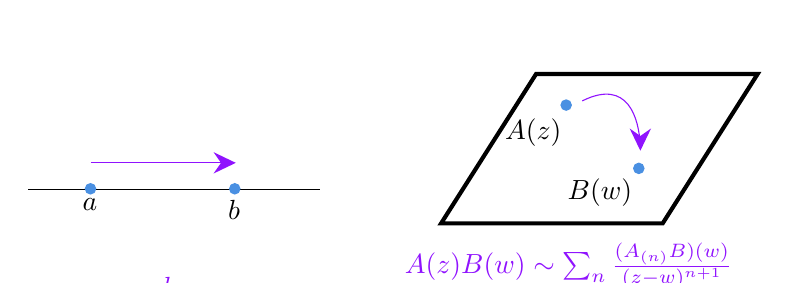
\begin{tikzpicture}[x=0.75pt,y=0.75pt,yscale=-1,xscale=1]

%Straight Lines [id:da21032606992521252] 
\draw    (35.58,72.83) -- (176.08,72.83) ;
%Shape: Circle [id:dp9501490203756839] 
\draw  [color={rgb, 255:red, 74; green, 144; blue, 226 }  ,draw opacity=1 ][fill={rgb, 255:red, 74; green, 144; blue, 226 }  ,fill opacity=1 ] (63.08,72.33) .. controls (63.08,70.95) and (64.2,69.83) .. (65.58,69.83) .. controls (66.96,69.83) and (68.08,70.95) .. (68.08,72.33) .. controls (68.08,73.71) and (66.96,74.83) .. (65.58,74.83) .. controls (64.2,74.83) and (63.08,73.71) .. (63.08,72.33) -- cycle ;
%Shape: Circle [id:dp8390430287126933] 
\draw  [color={rgb, 255:red, 74; green, 144; blue, 226 }  ,draw opacity=1 ][fill={rgb, 255:red, 74; green, 144; blue, 226 }  ,fill opacity=1 ] (132.58,72.33) .. controls (132.58,70.95) and (133.7,69.83) .. (135.08,69.83) .. controls (136.46,69.83) and (137.58,70.95) .. (137.58,72.33) .. controls (137.58,73.71) and (136.46,74.83) .. (135.08,74.83) .. controls (133.7,74.83) and (132.58,73.71) .. (132.58,72.33) -- cycle ;
%Straight Lines [id:da20373559830369148] 
\draw [color={rgb, 255:red, 144; green, 19; blue, 254 }  ,draw opacity=1 ]   (65.75,59.83) -- (132.58,59.83) ;
\draw [shift={(135.58,59.83)}, rotate = 180] [fill={rgb, 255:red, 144; green, 19; blue, 254 }  ,fill opacity=1 ][line width=0.08]  [draw opacity=0] (10.72,-5.15) -- (0,0) -- (10.72,5.15) -- (7.12,0) -- cycle    ;
%Shape: Parallelogram [id:dp8720886994320196] 
\draw  [line width=1.5]  (280.25,17.04) -- (387,17.04) -- (341.25,89) -- (234.5,89) -- cycle ;
%Shape: Circle [id:dp4710229132282462] 
\draw  [color={rgb, 255:red, 74; green, 144; blue, 226 }  ,draw opacity=1 ][fill={rgb, 255:red, 74; green, 144; blue, 226 }  ,fill opacity=1 ] (292.25,32) .. controls (292.25,30.62) and (293.37,29.5) .. (294.75,29.5) .. controls (296.13,29.5) and (297.25,30.62) .. (297.25,32) .. controls (297.25,33.38) and (296.13,34.5) .. (294.75,34.5) .. controls (293.37,34.5) and (292.25,33.38) .. (292.25,32) -- cycle ;
%Shape: Circle [id:dp34299194072766626] 
\draw  [color={rgb, 255:red, 74; green, 144; blue, 226 }  ,draw opacity=1 ][fill={rgb, 255:red, 74; green, 144; blue, 226 }  ,fill opacity=1 ] (327.25,62.5) .. controls (327.25,61.12) and (328.37,60) .. (329.75,60) .. controls (331.13,60) and (332.25,61.12) .. (332.25,62.5) .. controls (332.25,63.88) and (331.13,65) .. (329.75,65) .. controls (328.37,65) and (327.25,63.88) .. (327.25,62.5) -- cycle ;
%Curve Lines [id:da15903818606178466] 
\draw [color={rgb, 255:red, 144; green, 19; blue, 254 }  ,draw opacity=1 ]   (302.5,30) .. controls (324.7,18.9) and (329.79,38.6) .. (330.43,51.12) ;
\draw [shift={(330.5,54)}, rotate = 270] [fill={rgb, 255:red, 144; green, 19; blue, 254 }  ,fill opacity=1 ][line width=0.08]  [draw opacity=0] (10.72,-5.15) -- (0,0) -- (10.72,5.15) -- (7.12,0) -- cycle    ;

% Text Node
\draw (60.58,75.73) node [anchor=north west][inner sep=0.75pt]    {$a$};
% Text Node
\draw (130.58,76.73) node [anchor=north west][inner sep=0.75pt]    {$b$};
% Text Node
\draw (264.08,37.4) node [anchor=north west][inner sep=0.75pt]    {$A( z)$};
% Text Node
\draw (294.25,66.4) node [anchor=north west][inner sep=0.75pt]    {$B( w)$};
% Text Node
\draw (82.58,113.73) node [anchor=north west][inner sep=0.75pt]  [color={rgb, 255:red, 144; green, 19; blue, 254 }  ,opacity=1 ]  {$a\cdot b$};
% Text Node
\draw (215.75,97.4) node [anchor=north west][inner sep=0.75pt]  [color={rgb, 255:red, 144; green, 19; blue, 254 }  ,opacity=1 ]  {$A( z) B( w) \sim \sum _{n}\frac{( A_{( n)} B)( w)}{( z-w)^{n+1}}$};
% Text Node
\draw (359,20.4) node [anchor=north west][inner sep=0.75pt]    {$\bC$};
\end{tikzpicture}
\eea
On a plane, the ``product'' (binary operation) depends on the location holomorphically, leading to $\infty$-ly many binary operations.

\begin{defn}
A \textbf{vertex algebra} is a collection of data:
\begin{itemize}
    \item (space of states) a $\bZ$-graded superspace $\cV=\cV_0\oplus \cV_1$,
    \item (vacuum) a vector $\ket{0}\in \cV_0$,
    \item (translation operator) an even linear map $T: \cV\to\cV$,
    \item (state-field correspondence) an even linear operation (vertex operation) 
    \bea Y(-,z):\cV\to \on{End}\cV[[z,z^{-1}]], \quad A\mapsto Y(A,z)=\sum_{n\in\bZ} A_{(n)}z^{-n-1}\eea
    such that $Y(A,z)B\in \cV((z))$ for any $A,B\in \cV$. 
\end{itemize}
\end{defn}

The data are required to satisfy the following axioms:
\begin{itemize}
    \item (vacuum axiom) $Y(\ket{0},z)=1_{d_\cV}$, i.e. for any $A\in\cV$, 
    \bea Y(A,z)\ket{0}\in \cV[[z]] \quad \text{and} \quad \lim_{z\to0} Y(A,z)\ket{0}=A,\eea
    \item (translation axiom) $T\ket{0}=0$, i.e. for any $A\in\cV$, 
    \bea \lsb T,Y(A,z)\rsb=\p_z Y(A,z),\eea
    \item (locality axiom) all $\lcb Y(A,z)\rcb_{a\in\cV}$ are mutually local.
\end{itemize}

Roughly speaking, mutual locality implies that for any $A,B\in\cV$, we can expand as
\bea Y(A,z)Y(B,w)=\sum_{n\in\bZ}\frac{Y(A_{(n)}\cdot B,w)}{(z-w)^{n+1}}.\eea
This is called the \textbf{operator product expansion (OPE)}. $\lcb A_{(n)}\cdot B\rcb$ from the expansion coefficient can be viewed as defining an infinite tower of products. For simplicity, we will write
\bea A(z)\equiv Y(A,z) \quad \text{for }A\in\cV.\eea
Then the OPE can be written as
\bea A(z)B(w)=\sum_{n\in\bZ}\frac{A_{(n)}\cdot B(w)}{(z-w)^{n+1}}.\eea
We also write, whenever only the \emph{singular} parts matter, 
\bea A(z)B(w)\sim \sum_{n\geq 0}
\frac{A_{(n)}\cdot B(w)}{(z-w)^{n+1}}.\eea

Given a vertex algebra, we can define its \textbf{modes Lie algebra} 
\bea \oint \cV\coloneqq \on{Span}_{\bC}\lcb \oint dz\ z^k A(z)=A_{(k)}\rcb_{A\in\cV,\ k\in\bZ}.\eea
The Lie bracket of contour integrals is determined by the OPE,
\bea \lsb \oint dz\ z^m A(z),\ 
\oint dw\ w^n B(w)\rsb
=\oint dw\ w^n \oint_w dz\ z^m \sum_{j\in\bZ} \frac{A_{(j)}\cdot B(w)}{(z-w)^{j+1}},\eea
where only the singular part matters in the integration. The Lie bracket is represented diagrammatically as follows.
\bea 
\tikzset{every picture/.style={line width=0.75pt}}         
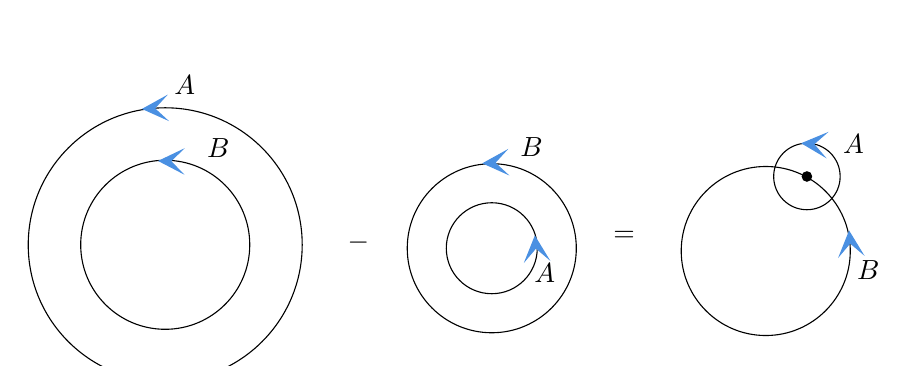
\begin{tikzpicture}[x=0.75pt,y=0.75pt,yscale=-1,xscale=1]


%Shape: Circle [id:dp4986409831322762] 
\draw   (49.33,109) .. controls (49.33,72.55) and (78.88,43) .. (115.33,43) .. controls (151.78,43) and (181.33,72.55) .. (181.33,109) .. controls (181.33,145.45) and (151.78,175) .. (115.33,175) .. controls (78.88,175) and (49.33,145.45) .. (49.33,109) -- cycle ;
%Shape: Circle [id:dp4714377376263692] 
\draw   (74.61,109) .. controls (74.61,86.51) and (92.84,68.28) .. (115.33,68.28) .. controls (137.82,68.28) and (156.06,86.51) .. (156.06,109) .. controls (156.06,131.49) and (137.82,149.72) .. (115.33,149.72) .. controls (92.84,149.72) and (74.61,131.49) .. (74.61,109) -- cycle ;
\draw  [color={rgb, 255:red, 74; green, 144; blue, 226 }  ,draw opacity=1 ][fill={rgb, 255:red, 74; green, 144; blue, 226 }  ,fill opacity=1 ] (115.78,48.51) -- (104.68,43.53) -- (115.32,37.64) -- (110.11,43.3) -- cycle ;
%Shape: Circle [id:dp3866837775378329] 
\draw   (250.75,110.67) .. controls (250.75,98.56) and (260.56,88.75) .. (272.67,88.75) .. controls (284.77,88.75) and (294.58,98.56) .. (294.58,110.67) .. controls (294.58,122.77) and (284.77,132.58) .. (272.67,132.58) .. controls (260.56,132.58) and (250.75,122.77) .. (250.75,110.67) -- cycle ;
%Shape: Circle [id:dp5310956184977278] 
\draw   (231.94,110.67) .. controls (231.94,88.18) and (250.18,69.94) .. (272.67,69.94) .. controls (295.16,69.94) and (313.39,88.18) .. (313.39,110.67) .. controls (313.39,133.16) and (295.16,151.39) .. (272.67,151.39) .. controls (250.18,151.39) and (231.94,133.16) .. (231.94,110.67) -- cycle ;
%Shape: Circle [id:dp15233205654865967] 
\draw   (408.48,76.1) .. controls (408.48,67.25) and (415.65,60.08) .. (424.5,60.08) .. controls (433.34,60.08) and (440.51,67.25) .. (440.51,76.1) .. controls (440.51,84.94) and (433.34,92.11) .. (424.5,92.11) .. controls (415.65,92.11) and (408.48,84.94) .. (408.48,76.1) -- cycle ;
%Shape: Circle [id:dp37578916230390047] 
\draw   (363.94,112) .. controls (363.94,89.51) and (382.18,71.28) .. (404.67,71.28) .. controls (427.16,71.28) and (445.39,89.51) .. (445.39,112) .. controls (445.39,134.49) and (427.16,152.72) .. (404.67,152.72) .. controls (382.18,152.72) and (363.94,134.49) .. (363.94,112) -- cycle ;
%Shape: Circle [id:dp21813935263931072] 
\draw  [fill={rgb, 255:red, 0; green, 0; blue, 0 }  ,fill opacity=1 ] (422.23,76.1) .. controls (422.23,74.84) and (423.24,73.83) .. (424.5,73.83) .. controls (425.75,73.83) and (426.76,74.84) .. (426.76,76.1) .. controls (426.76,77.35) and (425.75,78.36) .. (424.5,78.36) .. controls (423.24,78.36) and (422.23,77.35) .. (422.23,76.1) -- cycle ;
\draw  [color={rgb, 255:red, 74; green, 144; blue, 226 }  ,draw opacity=1 ][fill={rgb, 255:red, 74; green, 144; blue, 226 }  ,fill opacity=1 ] (123.26,74.24) -- (112.47,68.61) -- (123.45,63.36) -- (117.91,68.7) -- cycle ;
\draw  [color={rgb, 255:red, 74; green, 144; blue, 226 }  ,draw opacity=1 ][fill={rgb, 255:red, 74; green, 144; blue, 226 }  ,fill opacity=1 ] (279.78,74.71) -- (268.68,69.73) -- (279.32,63.84) -- (274.11,69.5) -- cycle ;
\draw  [color={rgb, 255:red, 74; green, 144; blue, 226 }  ,draw opacity=1 ][fill={rgb, 255:red, 74; green, 144; blue, 226 }  ,fill opacity=1 ] (432.75,66.32) -- (422.29,60.12) -- (433.53,55.46) -- (427.71,60.5) -- cycle ;
\draw  [color={rgb, 255:red, 74; green, 144; blue, 226 }  ,draw opacity=1 ][fill={rgb, 255:red, 74; green, 144; blue, 226 }  ,fill opacity=1 ] (440.35,113.98) -- (444.86,102.68) -- (451.19,113.07) -- (445.31,108.1) -- cycle ;
\draw  [color={rgb, 255:red, 74; green, 144; blue, 226 }  ,draw opacity=1 ][fill={rgb, 255:red, 74; green, 144; blue, 226 }  ,fill opacity=1 ] (288.95,116.38) -- (293.46,105.08) -- (299.79,115.47) -- (293.91,110.5) -- cycle ;

% Text Node
\draw (118.53,26) node [anchor=north west][inner sep=0.75pt]    {$A$};
% Text Node
\draw (134.27,56.6) node [anchor=north west][inner sep=0.75pt]    {$B$};
% Text Node
\draw (291.87,116.68) node [anchor=north west][inner sep=0.75pt]    {$A$};
% Text Node
\draw (285.2,55.87) node [anchor=north west][inner sep=0.75pt]    {$B$};
% Text Node
\draw (202,102.4) node [anchor=north west][inner sep=0.75pt]    {$-$};
% Text Node
\draw (330,101.07) node [anchor=north west][inner sep=0.75pt]    {$=$};
% Text Node
\draw (440.67,54.73) node [anchor=north west][inner sep=0.75pt]    {$A$};
% Text Node
\draw (447.39,115.4) node [anchor=north west][inner sep=0.75pt]    {$B$};
\end{tikzpicture}
\eea

\begin{eg}[$\beta\gamma$-system]
The $\beta\gamma$-system is generated by two \emph{bosonic} fields $\beta(z), \gamma(z)$ with the contractions
\bea \beta(z)\gamma(w)\sim \frac{\hbar}{z-w}\sim -\gamma(z)\beta(w).\eea
The vertex algebra $\cV$ is identified with the differential ring
\bea\cV= \nord{\bC[[\p^i\beta,\p^i\gamma]]} [[\hbar]],\eea
where $\nord{\ }$ is the \emph{normal ordering operator}. The general OPE is obtained via \textbf{Wick contractions}. For example,
\bea \nord{\beta(z)\gamma(z)} \nord{\beta(w)\gamma(w)}
&= \underbrace{\frac{\hbar}{z-w} \nord{\gamma(z)\beta(w)}- 
\frac{\hbar}{z-w} \nord{\beta(z)\gamma(w)}}_{\text{1 contraction}}
-\underbrace{\lb\frac{\hbar}{z-w}\rb^2}_{\text{2 contractions}}\\
&=\sum_{k\geq 0}\frac{\hbar}{z-w}\frac{(z-w)^k}{k!} \nord{\p^k\gamma(w)\beta(w)-\p^k\beta(w)\gamma(w)} -\frac{\hbar^2}{(z-w)^2}.\eea
\end{eg}

\begin{eg}[$bc$-system]
The $bc$-system is generated by two \emph{fermionic} fields $b(z), c(z)$ with
\bea b(z)c(w)\sim \frac{\hbar}{z-w}\sim c(z)b(w).\eea
The vertex algebra $\cV$ is identified with the differential ring
\bea\cV= \nord{\bC[[\p^i b,\p^i c]]} [[\hbar]].\eea
The general OPE is generated in the similar way as the $\beta\gamma$-system (but we need to take care of the signs). 
\end{eg}

More generally, we can define a general $\beta\gamma-bc$ system by considering a $\bZ_2$-graded space 
\bea h=h_0\oplus h_1\eea 
with an even symplectic pairing
\bea \lan -,-\ran: \asym^2 h\to \bC.\eea
Let $\lcb a_i\rcb$ be a basis of $h$, then we can define a vertex algebra $\cV_h$ by
\bea\cV_h= \nord{\bC[[\p^k a_i]]} [[\hbar]].\eea
The OPE is generated by
\bea a_i(z)a_j(w)\sim \frac{\hbar}{z-w} \lan a_i,a_j\ran.\eea
In particular, $h_0$ represents the copies of $\beta\gamma$-system; $h_1$ represents the copies of $bc$-system. 

\subsection{Chiral deformation of $\beta\gamma-bc$ systems}
We consider the following data:
\begin{itemize}
    \item an elliptic curve $E$ (topologically a torus $T^2$) with linear coordinate $z$ such that $z\sim z+1\sim z+\tau$,
    \item a graded symplectic space $h=h_0\oplus h_1$ with an even symplectic pairing $\lan -,-\ran$.
\end{itemize}
This defines a field theory in BV formalism by
\bea \begin{cases} \text{fields}:\ \cE=\Omega^{0,\blt}(E)\otimes h,\\
(-1)-\text{symplectic pair}: \omega(\varphi_1,\varphi_2)=\int_E dz\wedge \lan \varphi_1,\varphi_2\ran, \quad \varphi_i\in\cE. \end{cases}\eea
Note that $\omega$ has $\on{deg}=-1$ since we need exactly one $\ols{dz}$ from $\varphi_1,\varphi_2$ to be integrated.

The free theory is given by 
\bea \hf\int_E dz\lan \varphi
,\pb \varphi\ran, \quad \varphi\in\cE.\eea
The local quantum observables form exactly $\beta\gamma-bc$ system. Th propagator is given by \textbf{Szeg\H{o} kernel}
\bea \pb^{-1}\sim \frac{1}{z-w}+\text{regular}.\eea
We would like to consider a general interacting theory by turning on \textbf{chiral deformations}, such that we have
\bea \int \cL\lb \varphi,\p_z\varphi,\p_z^2\varphi,\cdots\rb\eea
which involves only \emph{holomorphic} derivatives. This is related precisely to the vertex algebra
\bea \cV_{h^\vee}= \bC[[\p^i h^\vee]] [[\hbar]]\eea
as follows. Define a map
\bea I: \cV_{h^\vee}\to \sO_{loc}(\cE), \quad \gamma\mapsto I_\gamma.\eea
Explicitly, if $\gamma=\sum \p^{k_1}a_1\cdots \p^{k_m}a_m$, then \bea I_\gamma(\varphi)=i\int_E dz \sum\pm \p^{k_1}_z a_1(\varphi)
\p^{k_m}_z a_m(\varphi).\eea
Here $a_i\in h^\vee$ and $a_i(\varphi)\in \omega^{0,\blt}(E)$.

\begin{thm}[UV finiteness]
For any $\gamma\in \cV_{h^\vee}$, the chiral deformed theory
\bea \hf \int_E dz\lan \varphi,\pb \varphi\ran +I_\gamma(\varphi)\eea
is \textbf{UV finite} in the sense that
\bea e^{\frac{1}{\hbar}I_\gamma[L]}=\lim_{\varepsilon\to 0} \exp{(\hbar P^L_\varepsilon)} e^{\frac{1}{\hbar}I_\gamma}\eea
exists.
\end{thm}

\begin{rmk}
The proof to the UV finiteness theorem is a bit technical. Interested reader may refer to \cite{Li:2016gcb}. The reason is different from topological QM, where we saw that the propagator is bounded (although not continuous). Here the graph integral is NOT absolute convergent. See the next section for a geometric interpretation of this fact.
\end{rmk}

Once we have a well-defined $I_\gamma[L]$ described above, we can formulate the \textbf{effective QME}
\bea \pb I_\gamma[L]+\hbar\Delta_L I_\gamma[L]+\hf\lcb I_\gamma[L],I_\gamma[L]\rcb_L=0\eea
and ask for the condition of $\gamma$ to satisfy the equation. It turns out that the answer is very simple.

\begin{thm}[Li \cite{Li:2016gcb}]
Consider $\gamma\in \cV_{h^\vee}$ and the effective functional $I_\gamma[L]$ defined above via the UV finiteness. Then $I_\gamma[L]$ satisfies the effective QME
\bea \pb I_\gamma[L]+\hbar\Delta_L I_\gamma[L]+\hf\lcb I_\gamma[L],I_\gamma[L]\rcb_L=0\eea
if and only if 
\bea \lsb \oint\gamma,\oint\gamma\rsb=0 \ \in \oint \cV.\eea
\end{thm}

\begin{rmk}
The local quantum observable of the chiral deformed theory is the vertex algebra $H^\blt(\cV_{h^\vee},\oint \gamma)$. So $\oint \gamma$ plays the role of BRST reduction. Reversely, vertex algebras coming from the BRST reduction of free field realizations can be realized via the model of chiral deformations above.
\end{rmk}

The above theorem can be glued for a \emph{chiral $\sigma$-model}
\bea \varphi:E\to X\eea
which produces a bundle $\cV(X)\to X$ of chiral vertex algebras on $X$. Then the solution of effective QME asks for a flat connection on $\cV(X)$ of the form
\bea D=d+\frac{1}{\hbar}\lsb \oint\gamma,-\rsb, \ \text{such that}\ D^2=0.\eea
Here $\gamma\in\Omega^1\lb X,\cV(X)\rb$ and $\oint \gamma$ is fiberwise chiral mode operator. This can be viewed as the \emph{chiral analogue of Fedosov connection}.

\section{Two-dimensional Chiral QFT-II}
\label{sec:2d2}

Recall that in \nameref{sec:2d1}, we discussed the (chiral) $\beta\gamma-bc$ system with the space of fields being the Dolbeault complex ($\varphi\in\Omega^{0,\blt}(\Sigma,h)$). The action functional is
\bea S=\underbrace{\hf\int\lan \varphi,\pb\varphi\ran}_{\text{free part}} \ +\underbrace{\int \cL(\p_z^\blt\varphi)}_{\text{chiral interaction, } I}\eea
The theory is UV finite, and the effective renormalized QME is simply described by $\lsb \oint \cL,\oint\cL\rsb=0$.

\subsection{Regularized integral and UV finiteness}
The propagator $\pb^{-1}$ is given by the Szeg\H{o} kernel which exhibits holomorphic poles $\frac{1}{z-w}$ along the diagonal. In general, the Feynman diagram involves $\int_{\Sigma^n} \Omega$, where $\Omega$ exhibits holomorphic poles of arbitrary order when $z_i\to z_j$.
It turns out that such looking divergent integral has an intrinsic \emph{regularization} via its conformal structure. 

For simplicity, we start by considering such an integral $\int_\Sigma \omega$.
Here $\Sigma$ is a Riemann surface, possibly with boundary $\p\Sigma$, $\omega$ is a 2-from on $\Sigma$ with meromorphic poles of arbitrary order along a finite set $D\subset\Sigma$, such that $D\cap\p\Sigma=\varnothing$.
\bea 
\tikzset{every picture/.style={line width=0.75pt}} 
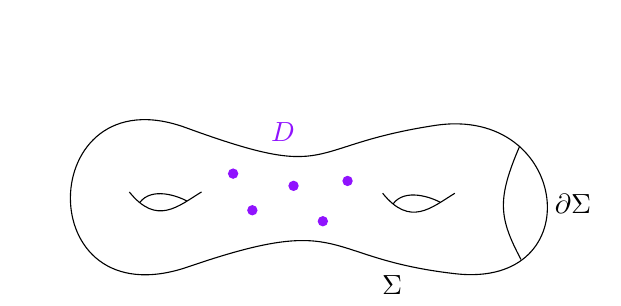
\begin{tikzpicture}[x=0.75pt,y=0.75pt,yscale=-1,xscale=1]

%Shape: Polygon Curved [id:ds035604419620915095] 
\draw   (79.37,25.97) .. controls (152.1,52.53) and (134.73,34.72) .. (199.52,24.9) .. controls (264.3,15.09) and (274.94,103.85) .. (209.22,96.35) .. controls (143.5,88.85) and (157.79,66.44) .. (80.63,93.01) .. controls (3.47,119.57) and (6.64,-0.59) .. (79.37,25.97) -- cycle ;
%Curve Lines [id:da7635811371660339] 
\draw    (52.17,56.96) .. controls (65.45,73.4) and (75.57,63.91) .. (86.95,56.96) ;
%Curve Lines [id:da8989271131706713] 
\draw    (57.23,62.02) .. controls (62.92,54.43) and (75.57,58.86) .. (80,61.39) ;
%Curve Lines [id:da5953645395125455] 
\draw    (174.23,57.59) .. controls (187.51,74.03) and (197.63,64.55) .. (209.01,57.59) ;
%Curve Lines [id:da4209585290119977] 
\draw    (179.29,62.65) .. controls (184.98,55.06) and (197.63,59.49) .. (202.06,62.02) ;
%Shape: Circle [id:dp3791131464091231] 
\draw  [color={rgb, 255:red, 144; green, 19; blue, 254 }  ,draw opacity=1 ][fill={rgb, 255:red, 144; green, 19; blue, 254 }  ,fill opacity=1 ] (99.98,48.13) .. controls (99.98,46.91) and (100.97,45.92) .. (102.19,45.92) .. controls (103.41,45.92) and (104.4,46.91) .. (104.4,48.13) .. controls (104.4,49.35) and (103.41,50.34) .. (102.19,50.34) .. controls (100.97,50.34) and (99.98,49.35) .. (99.98,48.13) -- cycle ;
%Shape: Ellipse [id:dp2374463332947847] 
\draw  [color={rgb, 255:red, 144; green, 19; blue, 254 }  ,draw opacity=1 ][fill={rgb, 255:red, 144; green, 19; blue, 254 }  ,fill opacity=1 ] (109.25,65.77) .. controls (109.25,64.55) and (110.23,63.57) .. (111.45,63.57) .. controls (112.67,63.57) and (113.66,64.55) .. (113.66,65.77) .. controls (113.66,66.99) and (112.67,67.98) .. (111.45,67.98) .. controls (110.23,67.98) and (109.25,66.99) .. (109.25,65.77) -- cycle ;
%Shape: Ellipse [id:dp35368836266522163] 
\draw  [color={rgb, 255:red, 144; green, 19; blue, 254 }  ,draw opacity=1 ][fill={rgb, 255:red, 144; green, 19; blue, 254 }  ,fill opacity=1 ] (129.09,54.01) .. controls (129.09,52.79) and (130.08,51.81) .. (131.3,51.81) .. controls (132.52,51.81) and (133.5,52.79) .. (133.5,54.01) .. controls (133.5,55.23) and (132.52,56.22) .. (131.3,56.22) .. controls (130.08,56.22) and (129.09,55.23) .. (129.09,54.01) -- cycle ;
%Shape: Ellipse [id:dp5744037578373786] 
\draw  [color={rgb, 255:red, 144; green, 19; blue, 254 }  ,draw opacity=1 ][fill={rgb, 255:red, 144; green, 19; blue, 254 }  ,fill opacity=1 ] (155.12,51.66) .. controls (155.12,50.44) and (156.1,49.45) .. (157.32,49.45) .. controls (158.54,49.45) and (159.53,50.44) .. (159.53,51.66) .. controls (159.53,52.88) and (158.54,53.86) .. (157.32,53.86) .. controls (156.1,53.86) and (155.12,52.88) .. (155.12,51.66) -- cycle ;
%Curve Lines [id:da3379921461483819] 
\draw    (240.29,34.8) .. controls (229.12,60.68) and (230.29,69.5) .. (240.88,89.49) ;
%Shape: Circle [id:dp9682521532873674] 
\draw  [color={rgb, 255:red, 144; green, 19; blue, 254 }  ,draw opacity=1 ][fill={rgb, 255:red, 144; green, 19; blue, 254 }  ,fill opacity=1 ] (143.21,71.07) .. controls (143.21,69.85) and (144.2,68.86) .. (145.41,68.86) .. controls (146.63,68.86) and (147.62,69.85) .. (147.62,71.07) .. controls (147.62,72.28) and (146.63,73.27) .. (145.41,73.27) .. controls (144.2,73.27) and (143.21,72.28) .. (143.21,71.07) -- cycle ;

% Text Node
\draw (172.73,96.1) node [anchor=north west][inner sep=0.75pt]    {$\Sigma $};
% Text Node
\draw (255.91,56.85) node [anchor=north west][inner sep=0.75pt]    {$\partial \Sigma $};
% Text Node
\draw (119.18,22.22) node [anchor=north west][inner sep=0.75pt]  [color={rgb, 255:red, 144; green, 19; blue, 254 }  ,opacity=1 ]  {$D$};
\end{tikzpicture}
\eea

Let $p\in D$ and $z$ be a local coordinate centered at $p$. Then locally $\omega$ can be written as
\bea \omega=\frac{\eta}{z^n}\eea
where $\eta$ is smooth, and $n\in \bZ$.
Since the pole order can be arbitrarily large, the naive $\int_\Sigma\omega$ is divergent in general. One intrinsic way out of this divergence problem \cite{Li:2020ljm} is as follows.
We can decompose $\omega$ into
\bea \omega=\alpha+\p\beta,\eea
where $\alpha$ is a 2-form with at most \emph{logarithmic pole} along $D$, $\beta$ is a $(0,1)$-form with \emph{arbitrary order of poles} along $D$, and $\p=dz\frac{\p}{\p z}$ is the holomorphic de Rham differential. 

\begin{rmk}
Such a decomposition \emph{exists} and is \emph{not unique}.
\end{rmk}

\begin{defn}[L-Zhou \cite{Li:2020ljm}]
Define the \textbf{regularized integral} 
\bea\dint_\Sigma\omega\coloneqq\int_\Sigma\alpha+\int_{\p\Sigma}\beta\eea
as a recipe to integrate the singular form $\omega$ on $\Sigma$, such that
\begin{itemize}
    \item it does NOT depend on the choice of $\alpha,\beta$,
    \item $\dint_\Sigma$ is invariant under conformal transformations,
    \item $\dint_\Sigma\p(-)=\int_{\p\Sigma}(-)$, 
    \item $\dint_\Sigma\pb(-)=\on{Res}(-)$.
\end{itemize}
\end{defn}
The regularized integral extends the usual integral for smooth forms, i.e., the following diagram is commutative:
\bea \begin{tikzcd}
\cA^2(\Sigma) \ar[rr, hook] \ar[dr, swap, "\int_\Sigma"]
&  & \cA^2(\Sigma,\star D) \ar[dl, "\dint_\Sigma"]\\
& \bC & 
\end{tikzcd}\eea

We can use this to define integrals on configuration space of $\Sigma$
\bea \on{Conf}_n(\Sigma)=\Sigma^n-\Delta =\lcb\left. (p_1,\cdots,p_n)\in\Sigma^n \right| p_i \neq p_j, \forall i\neq j\rcb\eea
and define
\bea\dint_{\Sigma^n} : \cA^{2n}(\Sigma^n,\star\Delta)\to \bC\eea
by
\bea \dint_{\Sigma^n}(-)= \dint_{\Sigma_1}\dint_{\Sigma_2}\cdots\ \dint_{\Sigma_n}(-).\eea
It does NOT depend on the choice of the ordering of the factors in $\Sigma^n$; Fubini-type theorem holds.
This gives an intrinsically regularized meaning for $\dint_{\Sigma^n} \Omega$, where $\Omega$ is the Feynman diagram integrand. 
This explains why the theory is UV finite.

\subsection{Homological structure of BV quantization}
Roughly speaking, BV quantization in QFT leads to \begin{itemize}
    \item factorization algebra $\on{Obs}$ of observables  \cite{costello2021factorization},
    \item a chain complex $\lb C_\blt(\on{Obs}),d\rb$ via algebraic structure of $\on{Obs}$,
    \item a BV algebra $\lb \cA,\Delta\rb$ describing the zero modes (at $L=\infty$) with a BV integration map
    \bea \int_{BV}: \cA\to \bC,\eea
    \item a $\bC[[\hbar]]$-linear map
    \bea \lan -\ran: C_\blt(\on{Obs})\to \cA((\hbar))\eea
    which is the HRG flow from $L=0$ to $L=\infty$ satisfying the QME $(d+\hbar\Delta)\lan -\ran=0$; the QME says that $\lan -\ran$ is a chain map intertwining $d$ and $\hbar\Delta$,
    \item partition function leading to the index theorem 
    \bea \on{Index}=\int_{BV}\lan 1\ran.\eea
\end{itemize}

Recall in the example of TQM,
we have the following data.
\begin{itemize}
    \item The factorization algebra is the Weyl algebra: $\on{Obs}=\cW_{2n}$.
    \item The factorization complex is the Hochschild chain complex $\lb C_\blt(\on{Obs}),d\rb$.
    \item BV algebra on zero modes: $\lb\cA,\Delta\rb=\lb \Omega^\blt(\bR^{2n}),\cL_{\omega^{-1}}\rb.$
    \item Free correlation map 
    \bea \lan -\ran: C_{\blt}(\cW_{2n})\to \Omega^\blt(\bR^{2n})((\hbar)), \quad b\mapsto \hbar \cL_{\omega^{-1}}.\eea
    \item $\on{Index}=\int_{BV}\lan 1\ran=\lsb e^{\omega_\hbar/\hbar}\widehat{A}\rsb$.
\end{itemize}
In the example of a 2d chiral QFT, we will have a similar story. \textsc{References}:
\cite{Gui:2021dci}.

\subsection{Beilinson-Drinfeld's chiral chain complex}
Intuitively, chiral chain complex can be viewed as a 2d chiral analogue of Hochschild chain complex.
\bea 
\tikzset{every picture/.style={line width=0.75pt}}
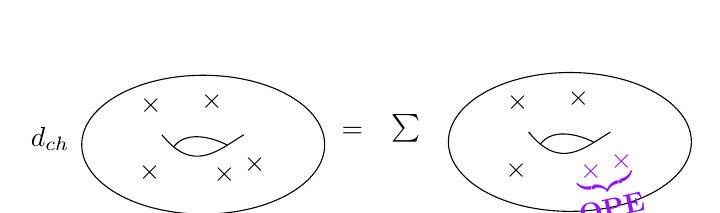
\begin{tikzpicture}[x=0.75pt,y=0.75pt,yscale=-1,xscale=1]

%Curve Lines [id:da635337608272412] 
\draw    (99.3,113.01) .. controls (114.35,131.65) and (125.82,120.89) .. (138.73,113.01) ;
%Curve Lines [id:da011829695865262835] 
\draw    (105.03,118.74) .. controls (111.49,110.14) and (125.82,115.16) .. (130.84,118.03) ;
%Shape: Ellipse [id:dp6950451999185667] 
\draw   (60.67,117.78) .. controls (60.67,99.31) and (86.87,84.33) .. (119.19,84.33) .. controls (151.52,84.33) and (177.72,99.31) .. (177.72,117.78) .. controls (177.72,136.25) and (151.52,151.22) .. (119.19,151.22) .. controls (86.87,151.22) and (60.67,136.25) .. (60.67,117.78) -- cycle ;
%Curve Lines [id:da5951843766986344] 
\draw    (275.96,111.67) .. controls (291.02,130.31) and (302.49,119.56) .. (315.4,111.67) ;
%Curve Lines [id:da849863385797317] 
\draw    (281.7,117.41) .. controls (288.15,108.81) and (302.49,113.82) .. (307.51,116.69) ;
%Shape: Ellipse [id:dp5521894453900986] 
\draw   (237.33,116.44) .. controls (237.33,97.97) and (263.54,83) .. (295.86,83) .. controls (328.19,83) and (354.39,97.97) .. (354.39,116.44) .. controls (354.39,134.92) and (328.19,149.89) .. (295.86,149.89) .. controls (263.54,149.89) and (237.33,134.92) .. (237.33,116.44) -- cycle ;

% Text Node
\draw (87.56,93.07) node [anchor=north west][inner sep=0.75pt]    {$\times $};
% Text Node
\draw (116.89,91.07) node [anchor=north west][inner sep=0.75pt]    {$\times $};
% Text Node
\draw (86.89,125.73) node [anchor=north west][inner sep=0.75pt]    {$\times $};
% Text Node
\draw (122.89,126.4) node [anchor=north west][inner sep=0.75pt]    {$\times $};
% Text Node
\draw (137.51,121.43) node [anchor=north west][inner sep=0.75pt]    {$\times $};
% Text Node
\draw (34.89,108.07) node [anchor=north west][inner sep=0.75pt]    {$d_{ch}$};
% Text Node
\draw (264.22,91.73) node [anchor=north west][inner sep=0.75pt]    {$\times $};
% Text Node
\draw (293.56,89.73) node [anchor=north west][inner sep=0.75pt]    {$\times $};
% Text Node
\draw (263.56,124.4) node [anchor=north west][inner sep=0.75pt]    {$\times $};
% Text Node
\draw (299.56,125.07) node [anchor=north west][inner sep=0.75pt]  [color={rgb, 255:red, 144; green, 19; blue, 254 }  ,opacity=1 ]  {$\times $};
% Text Node
\draw (314.18,120.09) node [anchor=north west][inner sep=0.75pt]  [color={rgb, 255:red, 144; green, 19; blue, 254 }  ,opacity=1 ]  {$\times $};
% Text Node
\draw (184.67,108.07) node [anchor=north west][inner sep=0.75pt]    {$=$};
% Text Node
\draw (208.67,102.07) node [anchor=north west][inner sep=0.75pt]    {$\sum $};
% Text Node
\draw (295.31,134.74) node [anchor=north west][inner sep=0.75pt]  [color={rgb, 255:red, 144; green, 19; blue, 254 }  ,opacity=1 ,rotate=-347.56]  {$\underbrace{\ \ \ \ \ \ }_{\textbf{OPE}}$};
\end{tikzpicture}
\eea

\begin{itemize}
    \item \cite{zhu1994global} studies the space of genus 1 conformal blocks (i.e. the 0th elliptic chiral homology).
    \item \cite{beilinson2004chiral} explores the chiral homology for general algebraic curves.
    \item \cite{van2021chiral,van2021first} constructed explicit complexes expressing the 0th and 1st elliptic chiral homology.
\end{itemize}

\paragraph{The construction of Beilinson-Drinfeld.}
Given the following data:
\begin{itemize}
    \item a category of right $\cD$-modules $\cM(X)$ on $X=\Sigma$,
    \item a category of right $\cD$-modules $\cM(X^S)$ on $X^S$, such that each element $M \in\cM(X^S)$ is a collection that assigns every finite index set $I\in S$ a right $\cD$-module $\cM_{X^I}$ on the product $X^I$ satisfying certain compatibility conditions,
    \item there is an exact fully faithful embedding
    \bea \Delta^{(S)}_\star: \cM(X)\hookrightarrow \cM(X^S)\eea
    via the diagonal map $\Delta^{(I)}:X \hookrightarrow X^I$,
    \item $\cM(X^S)$ carries a (chiral) tensor structure $\otimes^{ch}$,
\end{itemize}
then a chiral algebra $\cA$ is a \textbf{Lie algebraic object} via $\Delta^{(S)}_\star$. 

\begin{rmk}
The chiral algebra $\cA$ collects all ``normal ordering operators.''
\end{rmk}

We consider the Chevalley-Eilenberg (CE) complex
\bea \lb C(\cA),d_{CE}\rb=\lb \bigoplus_{\blt>0} \sym^\blt_{\otimes^{ch}}\lb \Delta^{(S)}_\star\cA[1]\rb, d_{CE}\rb.\eea
The chiral homology for this complex is
\bea C^{ch}(X,\cA)=R\Gamma_{DR}(X^S, C(\cA)).\eea

We will focus on $\beta\gamma-bc$ system, where the vertex operator algebra (VOA) $\cV^{\beta\gamma-bc}$ is the chiral algebra $\cA^{\beta\gamma-bc}$.
\begin{thm}[Gui-L \cite{Gui:2021dci}]
Let $E$ be an elliptic curve. Then the HRG flow gives a map
\bea \lan -\ran_{2d}: C^{ch}(E,\cA^{\beta\gamma-bc})\to \cA((\hbar))\eea
satisfying the QME $(d_{ch}+\hbar\Delta)\lan -\ran_{2d}=0$.
Roughly speaking, $\lan -\ran$ is defined by
\bea \lan \cO_1\otimes\cdots\otimes\cO_n\ran_{2d}\coloneqq \dint_{E^n} \lan \cO_1(z_1)\cdots \cO_n(z_n) \ran\eea
where $\lan \cO_1(z_1)\cdots \cO_n(z_n) \ran$
is a local correlator given by the Feynman diagram, and $\dint_{E^n}$ is the regularized integral.
\end{thm}


\subsection{2d $\to$ 1d reduction}
We summarize our discussion as follows.
\begin{table}[!htpb]\centering
            \begin{tabular}{c|c}\toprule
            \textbf{1d TQM} & \textbf{2d chiral QFT}\\ \hline
            Associative algebra & Vertex/chiral algebra\\ \hline
            Hochschild homology & Chiral homology\\ \hline 
            QME $(\hbar\Delta+b)\lan -\ran_{1d}=0$ & QME $(\hbar\Delta+d_{ch})\lan -\ran_{2d}=0$ \\ \hline
            $\lan \cO_1\otimes\cdots\otimes\cO_n\ran_{1d}=\int_{\ols{\on{Conf}_n(S^1)}}$ & $\lan \cO_1\otimes\cdots\otimes\cO_n\ran_{2d}=\dint_{\Sigma^n}$ \\ 
            \bottomrule
            \end{tabular}
\end{table}

In physics, the partition functions/correlation functions on elliptic curves are described by QM on $S^1$.
\bea 
\tikzset{every picture/.style={line width=0.75pt}}       
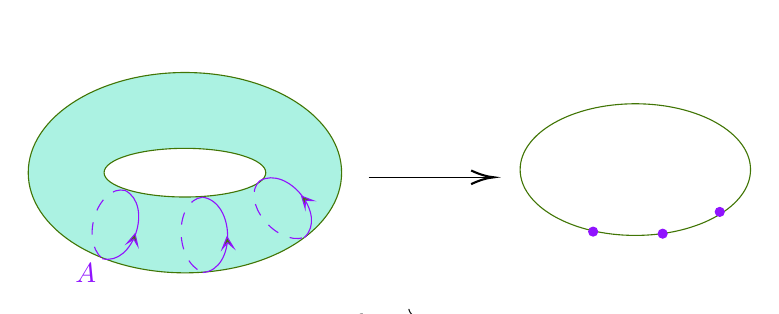
\begin{tikzpicture}[x=0.75pt,y=0.75pt,yscale=-1,xscale=1]

%Shape: Ellipse [id:dp4418092526097801] 
\draw  [color={rgb, 255:red, 65; green, 117; blue, 5 }  ,draw opacity=1 ] (321.5,63.79) .. controls (321.5,46.27) and (346.35,32.07) .. (377,32.07) .. controls (407.65,32.07) and (432.5,46.27) .. (432.5,63.79) .. controls (432.5,81.3) and (407.65,95.5) .. (377,95.5) .. controls (346.35,95.5) and (321.5,81.3) .. (321.5,63.79) -- cycle ;
%Straight Lines [id:da6931809500773398] 
\draw    (248.5,67.5) -- (306.83,67.5) ;
\draw [shift={(308.83,67.5)}, rotate = 180] [color={rgb, 255:red, 0; green, 0; blue, 0 }  ][line width=0.75]    (10.93,-3.29) .. controls (6.95,-1.4) and (3.31,-0.3) .. (0,0) .. controls (3.31,0.3) and (6.95,1.4) .. (10.93,3.29)   ;
%Shape: Circle [id:dp9584222087677268] 
\draw  [color={rgb, 255:red, 144; green, 19; blue, 254 }  ,draw opacity=1 ][fill={rgb, 255:red, 144; green, 19; blue, 254 }  ,fill opacity=1 ] (354.5,93.67) .. controls (354.5,92.47) and (355.47,91.5) .. (356.67,91.5) .. controls (357.86,91.5) and (358.83,92.47) .. (358.83,93.67) .. controls (358.83,94.86) and (357.86,95.83) .. (356.67,95.83) .. controls (355.47,95.83) and (354.5,94.86) .. (354.5,93.67) -- cycle ;
%Shape: Circle [id:dp8524982473210796] 
\draw  [color={rgb, 255:red, 144; green, 19; blue, 254 }  ,draw opacity=1 ][fill={rgb, 255:red, 144; green, 19; blue, 254 }  ,fill opacity=1 ] (388,94.67) .. controls (388,93.47) and (388.97,92.5) .. (390.17,92.5) .. controls (391.36,92.5) and (392.33,93.47) .. (392.33,94.67) .. controls (392.33,95.86) and (391.36,96.83) .. (390.17,96.83) .. controls (388.97,96.83) and (388,95.86) .. (388,94.67) -- cycle ;
%Shape: Circle [id:dp1755796687587492] 
\draw  [color={rgb, 255:red, 144; green, 19; blue, 254 }  ,draw opacity=1 ][fill={rgb, 255:red, 144; green, 19; blue, 254 }  ,fill opacity=1 ] (415.5,84.17) .. controls (415.5,82.97) and (416.47,82) .. (417.67,82) .. controls (418.86,82) and (419.83,82.97) .. (419.83,84.17) .. controls (419.83,85.36) and (418.86,86.33) .. (417.67,86.33) .. controls (416.47,86.33) and (415.5,85.36) .. (415.5,84.17) -- cycle ;
%Shape: Donut [id:dp07063864397558173] 
\draw  [color={rgb, 255:red, 65; green, 117; blue, 5 }  ,draw opacity=1 ][fill={rgb, 255:red, 80; green, 227; blue, 194 }  ,fill opacity=0.48 ,even odd rule] (121.03,65.26) .. controls (121.03,58.79) and (138.48,53.54) .. (160,53.54) .. controls (181.52,53.55) and (198.96,58.8) .. (198.96,65.28) .. controls (198.96,71.75) and (181.52,77) .. (160,77) .. controls (138.48,76.99) and (121.03,71.74) .. (121.03,65.26)(84.5,65.26) .. controls (84.51,38.61) and (118.31,17.01) .. (160.01,17.01) .. controls (201.7,17.02) and (235.5,38.63) .. (235.49,65.28) .. controls (235.49,91.93) and (201.68,113.53) .. (159.99,113.53) .. controls (118.29,113.52) and (84.5,91.91) .. (84.5,65.26) ;
%Curve Lines [id:da0009892278601366655] 
\draw [color={rgb, 255:red, 144; green, 19; blue, 254 }  ,draw opacity=1 ]   (196,69.19) .. controls (209.5,61.53) and (229,86.03) .. (217.5,96.53) ;
%Curve Lines [id:da44799976092621097] 
\draw [color={rgb, 255:red, 144; green, 19; blue, 254 }  ,draw opacity=1 ] [dash pattern={on 4.5pt off 4.5pt}]  (196,69.19) .. controls (186.5,78.53) and (203.5,100.53) .. (217.5,96.53) ;
\draw  [color={rgb, 255:red, 144; green, 19; blue, 254 }  ,draw opacity=1 ][fill={rgb, 255:red, 65; green, 117; blue, 5 }  ,fill opacity=1 ] (217.89,82.25) -- (216.27,76.66) -- (221.72,78.72) -- (218.04,78.57) -- cycle ;
%Curve Lines [id:da04657738471784345] 
\draw [color={rgb, 255:red, 144; green, 19; blue, 254 }  ,draw opacity=1 ]   (168.5,77.07) .. controls (184.43,79.43) and (184.7,112.12) .. (168.59,113.38) ;
%Curve Lines [id:da24828006383038592] 
\draw [color={rgb, 255:red, 144; green, 19; blue, 254 }  ,draw opacity=1 ] [dash pattern={on 4.5pt off 4.5pt}]  (168.5,77.07) .. controls (154.77,78.65) and (154.6,107.68) .. (168.59,113.38) ;
\draw  [color={rgb, 255:red, 144; green, 19; blue, 254 }  ,draw opacity=1 ][fill={rgb, 255:red, 65; green, 117; blue, 5 }  ,fill opacity=1 ] (178.04,101.88) -- (180.29,96.23) -- (183.42,101.43) -- (180.51,98.94) -- cycle ;
%Curve Lines [id:da43201889595924503] 
\draw [color={rgb, 255:red, 144; green, 19; blue, 254 }  ,draw opacity=1 ]   (131.17,73.82) .. controls (144.86,80.83) and (135.11,110.48) .. (120.16,106.69) ;
%Curve Lines [id:da5919508883701639] 
\draw [color={rgb, 255:red, 144; green, 19; blue, 254 }  ,draw opacity=1 ] [dash pattern={on 4.5pt off 4.5pt}]  (131.17,73.82) .. controls (118.27,71.06) and (109.24,97.26) .. (120.16,106.69) ;
\draw  [color={rgb, 255:red, 144; green, 19; blue, 254 }  ,draw opacity=1 ][fill={rgb, 255:red, 65; green, 117; blue, 5 }  ,fill opacity=1 ] (132.22,99.18) -- (135.98,94.76) -- (137.22,100.42) -- (135.35,97.28) -- cycle ;

% Text Node
\draw (223.5,128.9) node [anchor=north west][inner sep=0.75pt]    {$\lan - \ran_{2d} \longrightarrow \Tr_{\cH}\ \lan\cdots\ran$};
% Text Node
\draw (106,107.59) node [anchor=north west][inner sep=0.75pt]  [color={rgb, 255:red, 144; green, 19; blue, 254 }  ,opacity=1 ]  {$A$};
\end{tikzpicture}
\eea
Now we can define 2d correlation function using \emph{regularized integral} $\dint_E$. In 1d, operators are described by $A$-cycle $\oint_A$. These two integrals are not exactly the same, but related to each other by \emph{holomorphic anomaly}.

\begin{thm}[L-Zhou \cite{Li:2020ljm}]
Let $\Phi(z_1,\cdots,z_n;\tau)$ be a meromorphic elliptic function on $\bC^n\times \bH$ which is holomorphic away from diagonals. Let $A_1,\cdots,A_n$ be $n$ disjoint $A$-cycles on the elliptic curve $E_\tau=\bC/(\bZ\oplus \tau\bZ)$. 
\bea 
\tikzset{every picture/.style={line width=0.75pt}} 
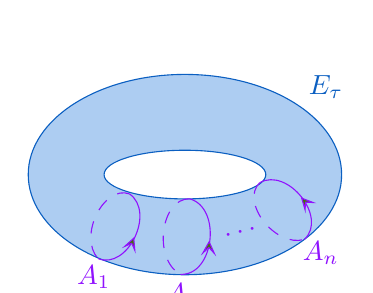
\begin{tikzpicture}[x=0.75pt,y=0.75pt,yscale=-1,xscale=1]
%Shape: Donut [id:dp6629776521166959] 
\draw  [color={rgb, 255:red, 11; green, 95; blue, 193 }  ,draw opacity=1 ][fill={rgb, 255:red, 74; green, 144; blue, 226 }  ,fill opacity=0.45 ,even odd rule] (244.53,97.57) .. controls (244.53,91.09) and (261.98,85.84) .. (283.5,85.85) .. controls (305.02,85.85) and (322.46,91.11) .. (322.46,97.58) .. controls (322.46,104.06) and (305.02,109.31) .. (283.5,109.3) .. controls (261.98,109.3) and (244.53,104.05) .. (244.53,97.57)(208,97.56) .. controls (208.01,70.91) and (241.81,49.31) .. (283.51,49.32) .. controls (325.2,49.33) and (359,70.94) .. (358.99,97.59) .. controls (358.99,124.24) and (325.18,145.84) .. (283.49,145.83) .. controls (241.79,145.83) and (208,124.21) .. (208,97.56) ;
%Curve Lines [id:da724728305831202] 
\draw [color={rgb, 255:red, 144; green, 19; blue, 254 }  ,draw opacity=1 ]   (319.5,101.5) .. controls (333,93.83) and (352.5,118.33) .. (341,128.83) ;
%Curve Lines [id:da09375441458438294] 
\draw [color={rgb, 255:red, 144; green, 19; blue, 254 }  ,draw opacity=1 ] [dash pattern={on 4.5pt off 4.5pt}]  (319.5,101.5) .. controls (310,110.83) and (327,132.83) .. (341,128.83) ;
\draw  [color={rgb, 255:red, 144; green, 19; blue, 254 }  ,draw opacity=1 ][fill={rgb, 255:red, 65; green, 117; blue, 5 }  ,fill opacity=1 ] (341.39,114.56) -- (339.77,108.96) -- (345.22,111.03) -- (341.54,110.88) -- cycle ;
%Curve Lines [id:da3775426299589082] 
\draw [color={rgb, 255:red, 144; green, 19; blue, 254 }  ,draw opacity=1 ]   (285.75,109.23) .. controls (301.43,113.61) and (297.57,146.42) .. (281.26,145.65) ;
%Curve Lines [id:da43322948676756656] 
\draw [color={rgb, 255:red, 144; green, 19; blue, 254 }  ,draw opacity=1 ] [dash pattern={on 4.5pt off 4.5pt}]  (285.75,109.23) .. controls (271.79,109.09) and (267.95,138.17) .. (281.26,145.65) ;
\draw  [color={rgb, 255:red, 144; green, 19; blue, 254 }  ,draw opacity=1 ][fill={rgb, 255:red, 65; green, 117; blue, 5 }  ,fill opacity=1 ] (292.18,135.31) -- (295.16,129.94) -- (297.64,135.54) -- (295.04,132.68) -- cycle ;
%Curve Lines [id:da9527348448178135] 
\draw [color={rgb, 255:red, 144; green, 19; blue, 254 }  ,draw opacity=1 ]   (256.75,106.87) .. controls (269.43,115.57) and (255.96,143.72) .. (241.61,138.05) ;
%Curve Lines [id:da12633292871659774] 
\draw [color={rgb, 255:red, 144; green, 19; blue, 254 }  ,draw opacity=1 ] [dash pattern={on 4.5pt off 4.5pt}]  (256.75,106.87) .. controls (244.31,102.47) and (231.99,127.3) .. (241.61,138.05) ;
\draw  [color={rgb, 255:red, 144; green, 19; blue, 254 }  ,draw opacity=1 ][fill={rgb, 255:red, 65; green, 117; blue, 5 }  ,fill opacity=1 ] (254.53,132.14) -- (258.83,128.25) -- (259.34,134.02) -- (257.88,130.66) -- cycle ;

% Text Node
\draw (230.33,140.23) node [anchor=north west][inner sep=0.75pt]  [color={rgb, 255:red, 144; green, 19; blue, 254 }  ,opacity=1 ]  {$A_{1}$};
% Text Node
\draw (310.43,125.53) node  [color={rgb, 255:red, 144; green, 19; blue, 254 }  ,opacity=1 ,rotate=-346.47]  {$\cdots $};
% Text Node
\draw (339,128.4) node [anchor=north west][inner sep=0.75pt]  [color={rgb, 255:red, 144; green, 19; blue, 254 }  ,opacity=1 ]  {$A_{n}$};
% Text Node
\draw (273,148.9) node [anchor=north west][inner sep=0.75pt]  [color={rgb, 255:red, 144; green, 19; blue, 254 }  ,opacity=1 ]  {$A_{2}$};
% Text Node
\draw (342,48.4) node [anchor=north west][inner sep=0.75pt]  [color={rgb, 255:red, 11; green, 95; blue, 193 }  ,opacity=1 ]  {$E_{\tau }$};
\end{tikzpicture}
\eea
Then the regularized integral 
\bea\dint_{E^n_\tau}\lb \prod_{i=1}^n \frac{d^2z_i}{\Im \tau}\rb \Phi(z_1,\cdots,z_n;\tau)\eea
lies in $\sO_{\bH}\lsb\frac{1}{\Im \tau}\rsb$. Moreover, we have
\bea\lim_{\ols{\tau}\to\infty}\dint_{E^n_\tau} \lb \prod_{i=1}^n\frac{d^2z_i}{\Im \tau}\rb \Phi
=\frac{1}{n!}\sum_{\sigma\in S_n}\int_{A_{\sigma(1)}} dz_1 \cdots \int_{A_{\sigma(n)}} dz_n\ \Phi,\eea
where $S_n$ is the permutation group for $n$.
Essentially this means
\bea\dint_{E^n}\xrightarrow{\lim_{\ols{\tau}\to\infty}} \text{averaged } \int_A,\eea
where $\dint_{E^n}$ is almost holomorphic modular, whereas the averaged $\int_A$ is quasi-modular.
\end{thm}
The anti-holomorphic dependence has a precise description.

\begin{thm}[L-Zhou \cite{Li:2020ljm}]
Let $\Phi$ be an almost-elliptic function. Then one has 
\bea \p_Y\dint_{E^n_\tau}\Phi= \dint_{E^n_\tau}\p_Y\Phi
-\sum_{i<j} \dint_{E^{n-1}_\tau}\on{Res}_{z_i=z_j}\lb(z_i-z_j)\Phi\rb.\eea
Here $Y=\frac{1}{\Im \tau}$.
This gives the \textbf{holomorphic anomaly equation}.
\end{thm}



\newpage
\bibliographystyle{hep}
\bibliography{ref}
\end{document}
